%%%%%%%%%%%%%%%%%%%%%%%%%%%%%%%%%%%%%%%%%
% Masters/Doctoral Thesis
% LaTeX Template
% Version 1.41 (9/9/13)
%
% This template has been downloaded from:
% http://www.latextemplates.com
%
% Original authors:
% Steven Gunn
% http://users.ecs.soton.ac.uk/srg/softwaretools/document/templates/
% and
% Sunil Patel
% http://www.sunilpatel.co.uk/thesis-template/
%
% License:
% CC BY-NC-SA 3.0 (http://creativecommons.org/licenses/by-nc-sa/3.0/)
%
% Note:
% Make sure to edit document variables in the Thesis.cls file
%
%%%%%%%%%%%%%%%%%%%%%%%%%%%%%%%%%%%%%%%%%

%----------------------------------------------------------------------------------------
%	PACKAGES AND OTHER DOCUMENT CONFIGURATIONS
%----------------------------------------------------------------------------------------

%\documentclass[11pt, twoside]{Thesis} % Paper size, default font size and two-sided paper

\documentclass[10 pt, a4paper, twoside, openright]{Thesis}
%\special{papersize=297mm,210mm}% it is A4 paper size, I got from Wikipedia.
\special{papersize=240mm,170mm}% it is the weird format of MPI thesis
\usepackage{glossaries}
\usepackage{blindtext}
\usepackage{titlesec}
\usepackage[T1]{fontenc}
\usepackage{lmodern}
\usepackage{textcomp}
\usepackage{tabularx}
\usepackage{tabu}
\usepackage{pdfx}
\usepackage{booktabs}
\usepackage{setspace}
\usepackage{multirow}
\usepackage{array}
\usepackage{booktabs}
\usepackage{bm}
\usepackage{afterpage}
\usepackage{longtable}
\usepackage{lscape}
%\usepackage{cite}
\usepackage{chngcntr}
\usepackage{url}
\urlstyle{same}
%\usepackage{fontspec}
%\newcommand{\TextUnderscore}{\rule{.2em}{.1pt}}
\DeclareGraphicsRule{.ai}{pdf}{.ai}{}
\DeclareGraphicsExtensions{.pdf,.png,.jpg,.ai,.eps}
\graphicspath{{Figures/}}
\usepackage[dvipsnames]{xcolor}
%\usepackage[sectionbib]{chapterbib}
\usepackage{textgreek}
\usepackage{float}
\usepackage{chemformula}
\usepackage{textcomp}
\usepackage{acronym}
\usepackage{wasysym}
\usepackage[english]{babel}
\usepackage[comma, sort&compress]{natbib} % Use the natbib reference package - read up on this to edit the reference style; if you want text (e.g. Smith et al., 2012) for the in-text references (instead of numbers), remove 'numbers'
\usepackage{caption}
\usepackage{pdfpages}
\usepackage{gensymb}
\usepackage{graphicx}
%\DeclareCaptionLabelFormat{myformat}{#1 #2}
%\captionsetup{within=none,labelformat=myformat}
\hypersetup{urlcolor=black, colorlinks=true} % Colors hyperlinks in blue - change to black if annoying
\title{\ttitle} % Defines the thesis title - don't touch this
%\usepackage[hmarginratio=2:3]{geometry}
\usepackage[titletoc]{appendix}

\titleformat{\chapter}[display]
  {\normalfont\bfseries}{}{0pt}{\Huge}

\makeglossaries{}

\newcommand{\beginsupplement}{%
        \setcounter{table}{0}
        \renewcommand{\thetable}{S\arabic{chapter}.\arabic{table}}%
        \setcounter{figure}{0}
        \renewcommand{\thefigure}{S\arabic{chapter}.\arabic{figure}}%
     }
\newcommand{\nosupplement}{%
        \setcounter{table}{0}
        \renewcommand{\thetable}{\arabic{chapter}.\arabic{table}}%
        \setcounter{figure}{0}
        \renewcommand{\thefigure}{\arabic{chapter}.\arabic{figure}}%
        }

\newcommand{\quotes}[1]{``#1"}

\begin{document}

\selectlanguage{english}
\sloppy
\frontmatter % Use roman page numbering style (i, ii, iii, iv...) for the pre-content pages

\setstretch{1.3} % Line spacing of 1.3

%try default
%\fancyhead[LE,RO]{\slshape \rightmark}
%\fancyhead[LO,RE]{\slshape \leftmark}
%\fancyfoot[C]{\thepage}
%\headrulewidth 0.4pt
%\footrulewidth 0 pt



% Define the page headers using the FancyHdr package and set up for one-sided printing
%\fancyhead{} % Clears all page headers and footers
%\usepackage{fancyhdr}
%\pagestyle{fancy}
%\fancyhead[RO,LE]{\thepage}
%\fancyhead[LE,RO]{\thepage}
%\rhead{\thepage} % Sets the right side header to show the page number
%\lhead{} % Clears the left side page header

%\pagestyle{fancy} % Finally, use the "fancy" page style to implement the FancyHdr headers

\newcommand{\HRule}{\rule{\linewidth}{0.5mm}} % New command to make the lines in the title page

% PDF meta-data
%\hypersetup{pdftitle={\ttitle}}
%\hypersetup{pdfsubject=\subjectname}
%\hypersetup{pdfauthor=\authornames}
%\hypersetup{pdfkeywords=\keywordnames}

%----------------------------------------------------------------------------------------
%	TITLE PAGE
%----------------------------------------------------------------------------------------

\begin{titlepage}

\begin{figure}
\hspace{-3.0cm}
\subfigure{\
\raggedright

\includegraphics[width=.4\textwidth]{Figures/MPI_logo.jpg}}
\hspace{6.5cm}
\subfigure{
\raggedleft

\includegraphics[width=.4\textwidth]{Figures/Unibremen_logo.png}}
\end{figure}



%\includegraphics[width = 40mm]{logo.jpg}


\begin{center}


%\vspace{2cm}

%\large Dissertation
\vspace*{2cm}



\large{\textbf{Master of Science Thesis:}}

\vspace{1cm}

%{\huge \textbf{\ttitle}\par}
{\LARGE\textbf{Ecological implications and characterization \\
 of genes of unknown function in the marine environment}\par}
\thispagestyle{empty}

%\vspace{1.5cm}
%The work of this thesis fulfills requirements \\
%for the degree of Master of Science in Marine Microbiology \\
%at the University of Bremen by Matthew S. Schechter. \\
\vspace{1.5cm}
University of Bremen\\
Max Planck Institute for Marine Microbiology \\
\large{Microbial Genomics and Bioinformatics Group} \\
\vspace{1.5cm}

\textbf{Matthew S. Schechter}
\vspace{2cm}
\vfill
{\large{March, 15, 2018}}\\[4cm] % Date

%\textsc{\LARGE \univname}\\[1.5cm] % University name
%\textsc{\Large Doctoral Thesis}\\[0.5cm] % Thesis type


%\HRule % Horizontal line

%{\huge \textbf{\ttitle}\par}% Thesis title

%\HRule % Horizontal line

%\begin{minipage}{0.4\textwidth}
%\begin{flushleft} \large
%\emph{Author:}\\

%\end{flushleft}
%\end{minipage}
%\begin{minipage}{0.4\textwidth}
%\begin{flushright} \large
%\emph{Supervisor:} \\

%\end{flushright}
%\end{minipage}\\[3cm]

%\vspace{2cm}

%\large Dissertation

%~\\zur Erlangung des Doktorgrades
%~\\der Naturwissenschaften
%~\\- Dr. rer. nat. - \\[0.3cm] % University requirement text
%\vspace{3cm}
%dem Fachbereich Biologie/Chemie
%~\\der Universit\"at Bremen
%~\\vorgelegt von

%\vspace{2.5cm}

%\vfill
\end{center}

\end{titlepage}

\newpage
\pagestyle{empty}


\begin{minipage}{0.3\textwidth}
\end{minipage} \hfill
\begin{minipage}{0.7\textwidth}
The work of this thesis fulfills requirements \\
for the degree of Master of Science in Marine Microbiology \\
at the University of Bremen by Matthew S. Schechter. \\
\end{minipage}


\null{}
\vfill{}

First evaluator: Prof. Dr. Frank Oliver Gl\"{o}ckner \\
Second evaluator: Dr. Pier Luigi Buttigieg \\
Supervisor: Dr. Antonio Fern\'{a}ndez-Guerra \\



%----------------------------------------------------------------------------------------
%	DECLARATION PAGE
%	Your institution may give you a different text to place here
%----------------------------------------------------------------------------------------

%\Declaration{

%\addtocontents{toc}{\vspace{1em}} % Add a gap in the Contents, for aesthetics

%I, \authornames, declare that this thesis titled, '\ttitle' and the work presented in it are my own. I confirm that:

%\begin{itemize}
%\item[\tiny{$\blacksquare$}] This work was done wholly or mainly while in candidature for a research degree at this University.
%\item[\tiny{$\blacksquare$}] Where any part of this thesis has previously been submitted for a degree or any other qualification at this University or any other institution, this has been clearly stated.
%\item[\tiny{$\blacksquare$}] Where I have consulted the published work of others, this is always clearly attributed.
%\item[\tiny{$\blacksquare$}] Where I have quoted from the work of others, the source is always given. With the exception of such quotations, this thesis is entirely my own work.
%%\item[\tiny{$\blacksquare$}] I have acknowledged all main sources of help.
%\item[\tiny{$\blacksquare$}] Where the thesis is based on work done by myself jointly with others, I have made clear exactly what was done by others and what I have contributed myself.\\
%\end{itemize}

%Signed:\\
%\rule[1em]{25em}{0.5pt} % This prints a line for the signature

%Date:\\
%\rule[1em]{25em}{0.5pt} % This prints a line to write the date
%}

\clearpage % Start a new page

%----------------------------------------------------------------------------------------
%	QUOTATION PAGE
%----------------------------------------------------------------------------------------

%\pagestyle{empty} % No headers or footers for the following pages

%\null\vfill\vfill\vfill\vfill % Add some space to move the quote down the page a bit


%\begin{flushright}
%Dedication goes here
%\end{flushright}

%\vfill\vfill\vfill\vfill\vfill\vfill\null{} % Add some space at the bottom to position the quote just right

%\clearpage % Start a new page

%\pagestyle{empty} % No headers or footers for the following pages

%\null\vfill % Add some space to move the quote down the page a bit

%\vfill\vfill\vfill\vfill\vfill\vfill\null{} % Add some space at the bottom to position the quote just right

%\clearpage % Start a new page
%\cleardoublepage{}

%----------------------------------------------------------------------------------------
%	ABSTRACT PAGE
%----------------------------------------------------------------------------------------

%\addtotoc{Summary} % Add the "Abstract" page entry to the Contents

%\abstract{\addtocontents{toc}{\vspace{1em}} % Add a gap in the Contents, for aesthetics



\clearpage % Start a new page

%----------------------------------------------------------------------------------------
%	ACKNOWLEDGEMENTS
%----------------------------------------------------------------------------------------

%\setstretch{1.3} % Reset the line-spacing to 1.3 for body text (if it has changed)

%\acknowledgements{\addtocontents{toc}{\vspace{1em}} % Add a gap in the Contents, for aesthetics

%The acknowledgements and the people to thank go here, don't forget to include your project advisor\ldots
%}
%\clearpage % Start a new page

%----------------------------------------------------------------------------------------
%	LIST OF CONTENTS/FIGURES/TABLES PAGES
%----------------------------------------------------------------------------------------

\pagestyle{fancy} % The page style headers have been "empty" all this time, now use the "fancy" headers as defined before to bring them back
\newpage
\chapter{Abstract}
\chaptermark{}
\renewcommand{\chaptermark}[1]{\markboth{#1}{}}
\renewcommand{\sectionmark}[1]{\markright{#1}}
\fancyhead[RE]{\small}
% Section in the left on even pages}
\fancyhead[LO]{\small\rightmark}%Section in the left on odd pages

The era of environmental metagenomic sequencing has added terabytes of sequencing data to databases. To explore this immense diversity to genes, clustering techniques have been used to group protein coding sequences into protein families (clusters). This has lead to the discovery of novel families and redefined protein diversity. Unfortunately, due to the lack of isolated microbial genomes from the environment and incorrect protein annotation management in databases, many protein families are left without a known function. This constrains microbial functional research and often the \quotes{unknowns} are discounted during microbial functional profiling. There have been many approaches to expand the annotations of known proteins to the unknowns, but still a large proportion of protein families remain uncharacterized. Additionally, there have been attempts to categorize and classify the unknown, but sufficient categories have not been described to include all unknown environmental protein coding sequences. The Vanni \textit{et. al.} (in prep) workflow takes a novel approach to protein clustering, focusing on cluster quality and categorization of the unknown clusters. In this thesis, the resulting clusters from Vanni \textit{et. al.} workflow were used to investigate the distribution and biogeography of the unknown in the TARA Oceans dataset. This investigation demonstrates that when utilizing the whole metagenomic sample (knowns and unknowns) there is increased variation in ordinations which leads to clearer sample site separation. It is also found that the unknown fraction of protein clusters have distinct characteristics of being adaptive proteins. Finally, evidence is presented of an ubiquitous unknown fraction of protein clusters throughout the world's oceans.
\cleardoublepage{}
%\newpage
\chapter{Zusammenfassung}
\chaptermark{}
\renewcommand{\chaptermark}[1]{\markboth{#1}{}}
\renewcommand{\sectionmark}[1]{\markright{#1}}
\fancyhead[RE]{\small}
% Section in the left on even pages}
%Section in the left on odd pages
\fancyhead[LO]{\small\rightmark}

A german summary goes here

\newpage
\clearpage % Start a new page
\thispagestyle{plain}
\section*{Abbreviations}
\setstretch{1} % Set the line spacing to 1.5, this makes the following tables easier to read

%\lhead{\emph{Abbreviations}} % Set the left side page header to "Abbreviations"

\begin{acronym}
%\acro{ABC}{ATP-binding cassette}
%\acro{ANI}{average nucleotide identity}
\acro{DUF}{Domain of Unknown Function}
\acro{EU}{Environmental Unknowns}
\acro{FAIR}{Findable Accessible Interoperable Reproducible}
\acro{GU}{Genomic Unknowns}
\acro{HMM}{Hidden Markov Model}
\acro{Kwp}{Knowns without PFAM annotation}
\acro{ORF}{Open Reading Frame}
\acro{OTU}{Operational Taxonomic Unit}
\acro{PCA}{Principal Component Analysis}
\acro{TP}{TARA Ocean prokaryotic metagenomes (all depths)}
\acro{TPS}{TARA Ocean prokaryotic, surface metagenomes}
\end{acronym}

\cleardoublepage{}
\clearpage % Start a new page
\thispagestyle{plain}
\section*{Glossary}
\setstretch{1} % Set the line spacing to 1.5, this makes the following tables easier to read

%\lhead{\emph{Abbreviations}} % Set the left side page header to "Abbreviations"

\begin{acronym}
\acro{Cluster}{A group of protein coding sequences that were grouped together by an unsupervised sequence clustering algorithm.}
\acro{Component}{A group of clusters from the Vanni et. al. workflow that were aggregated together due to PFAM domain architecture redundancy.}
\acro{Environmental Unknowns}{ORF clusters with an unknown function and are not found in sequenced or draft- genomes.}
\acro{Genomic Unknowns}{ORF clusters that have an unknown function (e.g. DUF, hypothetical protein) but are found in sequenced or draft-genomes.}
\acro{Knowns}{ORF clusters that have been annotated with a PFAM domains of known function.}
\acro{Knowns without PFAMs}{ORF clusters that have a known function but do not contain PFAM annotations.}
\end{acronym}


%\lhead{\emph{Table of Contents}} % Set the left side page header to "Contents"
\tableofcontents % Write out the Table of Contents

%\lhead{\emph{List of Figures}} % Set the left side page header to "List of Figures"
\listoffigures % Write out the List of Figures

%\lhead{\emph{List of Tables}} % Set the left side page header to "List of Tables"
\listoftables % Write out the List of Tables

%----------------------------------------------------------------------------------------
%	GLOSSARY
%----------------------------------------------------------------------------------------
%\LARGE{\textbf{Glossary}}


%\textbf{Clusters:} \textbf{W}hat (it) \textbf{S}tands \textbf{F}or \\
%\textbf{Components:}  \textbf{W}hat (it) \textbf{S}tands \textbf{F}or \\


%\newpage
%----------------------------------------------------------------------------------------
%	ABBREVIATIONS
%----------------------------------------------------------------------------------------
%\LARGE{Abbreviations}
%
%
%\textbf{TP}  \textbf{W}hat (it) \textbf{S}tands \textbf{F}or \\
%\textbf{TPS}  \textbf{W}hat (it) \textbf{S}tands \textbf{F}or \\
%
%\LARGE{Glossary}
%
%
%\textbf{Clusters:} \textbf{W}hat (it) \textbf{S}tands \textbf{F}or \\
%\textbf{Components:}  \textbf{W}hat (it) \textbf{S}tands \textbf{F}or \\

%----------------------------------------------------------------------------------------
%	PHYSICAL CONSTANTS/OTHER DEFINITIONS
%----------------------------------------------------------------------------------------

%\clearpage % Start a new page

%\lhead{\emph{Physical Constants}} % Set the left side page header to "Physical Constants"

%\listofconstants{lrcl} % Include a list of Physical Constants (a four column table)
%{
%Speed of Light & $c$ & $=$ & $2.997\ 924\ 58\times10^{8}\ \mbox{ms}^{-\mbox{s}}$ (exact)\\
% Constant Name & Symbol & = & Constant Value (with units) \\
%}

%----------------------------------------------------------------------------------------
%	SYMBOLS
%----------------------------------------------------------------------------------------

%\clearpage % Start a new page

%\lhead{\emph{Symbols}} % Set the left side page header to "Symbols"

%\listofnomenclature{lll} % Include a list of Symbols (a three column table)
%{
%$a$ & distance & m \\
%$P$ & power & W (Js$^{-1}$) \\
% Symbol & Name & Unit \\

%& & \\ % Gap to separate the Roman symbols from the Greek

%$\omega$ & angular frequency & rads$^{-1}$ \\
% Symbol & Name & Unit \\
%}

%----------------------------------------------------------------------------------------
%	DEDICATION
%----------------------------------------------------------------------------------------

\setstretch{1.3} % Return the line spacing back to 1.3

\pagestyle{empty} % Page style needs to be empty for this page

%\dedicatory{\ldots} % Dedication text

%\addtocontents{toc}{\vspace{2em}} % Add a gap in the Contents, for aesthetics

%----------------------------------------------------------------------------------------
%	THESIS CONTENT - CHAPTERS
%----------------------------------------------------------------------------------------

\mainmatter{}% Begin numeric (1,2,3...) page numbering

\pagestyle{fancy} % Return the page headers back to the "fancy" style

% Include the chapters of the thesis as separate files from the Chapters folder
% Uncomment the lines as you write the chapters
% Chapter 1
% Chapter Template
\chapter{Introduction} % Main chapter title
\label{Chapter1} % Change X to a consecutive number; for referencing this chapter elsewhere, use \ref{ChapterX}

%\lhead{Chapter 1. \emph{Introduction}} % Change X to a consecutive number; this is for the header on each page - perhaps a shortened title
\renewcommand{\chaptermark}[1]{\markboth{#1}{}}
\renewcommand{\sectionmark}[1]{\markright{#1}}
\fancyhead[RE]{\small\leftmark}
% Section in the left on even pages}
\fancyhead[LO]{\small\rightmark}%Section in the left on odd pages

%\section{A section goes here}

Evolution has yielded an immense diversity of microbial functions. Today, many of those functions remain uncharacterized and exploring the unknown taxa and functions of the world\textquotesingle s microbiomes should be a \quotes{central priority for biologists} \citep{Bernard_2018}. Even after a century of functional characterization of the model organism \textit{Saccharomyces cerevisiae}, greater than 30\% of its protein coding sequences do not have a clear function \citep{Ellens_2017}. To shed light on the unknown functions of the microbial world, an important first step is to categorize and quantify how much is already known and how much is not known. With modern sequencing technologies and large scale sampling projects, this is now possible.\\

The emerging fields of metagenomics and shotgun sequencing have allowed for the description of the total genetic content in environmental samples. Rather than amplifying specific target DNA sequences (i.e. amplicon studies), metagenomics has the potential to simultaneously unveil both function and taxonomy of the microorganisms present in a sample. This allows for the comparison and quantification of differences in microbial physiological traits between sites. With the onset of next generation sequencing (NGS), cost per sequence has dramatically decreased down to 1 cent per megabase (https://www.genome.gov/sequencingcostsdata/, accessed 12.03.2018). Owing to this, large scale metagenomics sampling projects such as Global Ocean Sampling (GOS) \citep{Rusch_2007}, TARA Oceans \citep{Sunagawa_2015}, and Ocean Sampling Day (OSD) \citep{Kopf_2015} have sampled the world\textquotesingle s oceans and added terabytes of novel sequence data to databases. \\

GOS was the first attempt to create a snapshot of ocean genetic diversity with some of the largest sampling transects and collections of metadata ever accomplished \citep{Rusch_2007}. Its dataset generated 6.12 million open reading frames (ORFs) from its Sanger sequencing long reads \citep{Yooseph_2007}. Additionally, the GOS dataset lead to fascinating insights into marine microbial ecology, including the elucidation of the ocean\textquotesingle s dominant microbial genomes (i.e. \textit{Prochlorococcus} and SAR-11) and uncovering more microbial diversity in the ocean than previously thought \citep{Nealson_2007, Venter_2004, Rusch_2007, Yooseph_2007}.\\

Inspired by the GOS dataset, The TARA Oceans Expedition went a step further, not only increasing the breadth of sampling, but adding a systematic exploration of the sunlit ocean with the addition of more filter fractions and depths, and unprecedented sequencing depth. The first analysis of the prokaryotic fraction of the TARA dataset yielded a 40 million non-redundant reference gene catalogue \citep{Sunagawa_2015}. Later, a metatranscriptome analysis of the eukaryotic fraction added a separate 116 million non-redundant reference gene catalogue \citep{Carradec_2018}. Investigation into the prokaryotic dataset uncovered temperature as the main driver of microbial function and diversity, and revealed that the core functionality of the ocean microbiome compared to the human microbiome is 73\% similar \citep{Sunagawa_2015}.\\

\textbf{From data to knowledge}\\

Microbial knowledge discovery from GOS and TARA would not have been possible without the ability for predicted genes (i.e. open reading frames - ORFs) to be annotated. With annotated ORFs, overall community functional fingerprints can be compared between samples. Analysis of the TARA ocean data revealed that upon aggregation of functions within metagenomes, there is functional redundancy throughout the world\textquotesingle s ocean \citep{Louca_2016}. Yet, due to the sheer number of ORFs generated from these datasets, in the recent years, a variety of tools have been developed to efficiently compare and annotate environmental sequences with characterized sequences in databases. Algorithmic improvements to the original BLAST program \citep{Altschul_1990}, like DIAMOND \citep{Buchfink_2014} or MMSEQS2 \citep{Steinegger_2017} have allowed for local alignments of query sequences against a target sequence database in a high-throughput manner. However, sequence similarity based annotation methods have limitations if the scientific question at hand is detecting remote homologies or accurately assigning function. In fact, sequence similarity does not inherently imply homology or function, but is merely a metric to describe nucleotide resemblance \citep{States_1991}. To detect functional similarity and/or investigate evolutionary based questions of proteins (e.g. homologues, paralogues, and conserved domains), profile based tools should additionally be used.\\

A common way to create protein profiles is by calculating Hidden Markov Models (HMM) from multiple sequence alignments (MSAs) of protein families. Pfam \citep{Finn_2015} is an example of a profile database that manually curates protein families of highly conserved functional regions within proteins called domains. Other examples of protein family profile databases are Clusters of Orthologous Genes (COG) \citep{Tatusov_2000}, SFams \citep{Sharpton_2012}, and eggNOG \citep{Huerta_Cepas_2015}. Protein profile databases differ in their curation methodology, but manual curation of protein families is the best way to ensure high quality. This is because an expert can add biological context to a protein family\textquotesingle s MSA and identify the spurious members. Unfortunately, due to the size of nucleotide databases and large metagenome projects, the amount of sequences now far outweighs the time constraints of manual definition and curation of protein families.\\

To handle this amount of data, unsupervised clustering algorithms are being used to define an initial set of related proteins. These algorithms follow two main approaches, graph based and sequence similarity based \citep{Pavlopoulos_2017}. Graph based clustering algorithms start by performing an all-versus-all alignment using tools like DIAMOND or BLAST. Next, they create a sequence similarity network (SSN) using on the criterion of the alignment (e.g. e-value) as edges, then perform a clustering of the SSN to extract components as protein families (MCL is an example of a popular method \citep{Enright_2002}). On the other hand, tools that are based on sequence similarity grouping use k-mer frequencies (MMSEQS2 \citep{Steinegger_2017}, CD-HIT \citep{Li_2006}, UCLUST \citep{Edgar_2010}). One characteristic of the latter methods is their increased speed. With this, they are well suited to be applied to the massive metagenomic data sets.\\

In fact, one way to explore protein family diversity of environmental metagenomic ORFs is to cluster them with already recovered ORFs sequences in databases. This can lead to previously characterized protein families being expanded, shrunk, or the creation of novel families. GOS took this approach and yielded 1,700 clusters (grouped sequences after clustering) with no detectable homology or function \citep{Yooseph_2007}. Although new families may emerge when including new sequences, some may have a known function, but a vast majority will remain unknown.\\

\textbf{De-bunking the unknown}\\

There have been different strategies to expand annotations to unknown protein families including protein structure/sequence similarity analysis and domain co-occurrence networks. \cite{Jaroszewski_2009} structurally characterized 250 PFAM domains of unknown function (DUFs) using structural genomics. After comparing DUFs to known proteins on a structural level, it was determined that most of the DUFs were distant variants and not completely novel. \cite{Mudgal_2015} expanded upon this work with increased sensitivity and higher quality structural databases which lead to 20\% of DUFs being annotated as distantly related domains. Both studies discuss that the protein universe may soon be saturated from a structural perspective and most \quotes{novel} sequences are due to protein diversification from environmental niche selection. Based on the assumption that DUFs are products of niche adaptation, \cite{Buttigieg_2013} postulated that DUFs may co-occur with domains of known function between metagenomic samples. To explore this, they calculated the co-occurrence of DUFs with characterized domains in the GOS dataset and used correlation and network exploration to infer function, i.e. \quotes{guilty by association} method.\\

Even after deploying different strategies to annotate functions to new protein families, some families remain unknown. It is then an important step to confirm clusters that do not have detectable homology or function, are indeed novel and legitimate biological entities. This is a unique challenge in metagenomic data due to short reads, insufficient sequencing depth \citep{Parks_2011, Barrientos_Somarribas_2018}. Moreover, gene prediction algorithms have limitations and can yield inaccurate ORFs predictions leading to spurious proteins, which can lead to spurious protein families. Dedicated databases have been curated to detect and remove spurious proteins (e.g. AntiFAM \citep{Eberhardt_2012}). Additionally, specific tools like Spurio \citep{H_ps_2018} have been designed to score query ORFs on their likelihood of being spurious.\\

Another strategy to confirm protein family novelty is to determine if the members of the cluster are under positive or negative selective pressure by calculating non-synonymous to synonymous substitutions (Ka/Ks) \citep{Yooseph_2007, Barrientos_Somarribas_2018}. If ORFs have a Ka/Ks value close to 1, there is a strong indication for no selective pressure, thus a predicted ORF may not be a real coding sequence \citep{Nekrutenko_2001}. One issue with this validation strategy is, it assumes that all proteins in a metagenomic sample are under the same environmental pressures. When filtering out novel clusters with the criteria of Ka/Ks being closed to one, an assumption is made that all proteins are under purifying selection.

\textbf{Categorizing the unknown}\\

Even after various strategies to expand annotations and debunk unknown clusters, numerous protein families still indeed remain with unknown functions. The concept of \quotes{unknowns} in microbiology is a recognized problem that has implications for both fundamental and applied biological research. The term \quotes{biological dark matter} was first used by \cite{Marcy_2007} to describe the uncultured majority of microbes that could only be indirectly detected via environmental sequencing methods. Later, the term would also be used to refer to protein families with no detectable homology to characterized proteins from sequenced genomes \citep{Ellens_2017, Perdig_o_2017, Roux_2015, Fischer_1999}.\\

When categorizing and defining the unknown, it is important to quantify in reality how much is already known. \cite{Perdig_o_2017} approached the unknowns from a structural perspective by making the \quotes{Dark Proteome Database}. Protein sequences are ranked on a scale of \quotes{darkness} based on how confidently parts or the whole sequence can have of an inferred 3D structure. This is done by calculating MSAs to protein structural databases. Wyman et al., 2017 categorized SFams (clusters created via a graph-based approach from sequences of genomes) as FUnkFams (protein families of unknown function) if the clusters could not be annotated by the Pfam or the NCBI Conserved Domain database.\\

For this thesis, I used the clusters of ORFs produced from the work of Vanni et. al. (in prep.)(\url{https://orcid.org/0000-e2-1124-1147}). This workflow builds upon the motivations of the methods mentioned above but focuses on ORF cluster validation and deeper categorization of the unknown. Vanni et. al. used MMSEQS2 to cluster the 322,248,552 ORFs from The Human Microbiome Project (HMP), TARA Oceans \citep{Sunagawa_2015}, Ocean Sampling Day (OSD) \citep{Kopf_2015}, Global Ocean Sampling Expedition (GOS) \citep{Yooseph_2007}, and Malaspina \citep{Duarte_2015}. This dataset yielded 32,465,074 clusters that were then validated downstream. In parallel to clustering, the ORF dataset received Pfam annotations which were used to assist in cluster validation and unknown categorization.\\

Cluster validation is a critical step to protein clustering because unsupervised clustering algorithms can include non-biologically relevant ORFs into clusters due to incomplete or spurious ORFs gene duplications, and genome rearrangements. Vanni et. al. validated clusters for compositional and functional homogeneity. At the end of the validation steps, 2,953,903 clusters were successfully passed on to be categorized in terms of their level of unknown.\\

The goal of the categorization was to quantify the amount of novel versus characterized clusters based on the ability to annotate their function. For this purpose, the ORF cluster space was classified in the following categories:\\

\textbf{Knowns with PFAM (Knowns)}\\
ORF clusters that have been annotated with a PFAM domains of known function.\\
\textbf{Knowns without PFAMs (Kwp)}\\
ORF clusters that have a known function but do not contain PFAM annotations.\\
\textbf{Genomic Unknowns (GUs)}\\
ORF clusters that have an unknown function (e.g. DUF, hypothetical protein) but are found in sequenced or draft-genomes.\\
\textbf{Environmental Unknowns (EUs)}\\
ORF clusters with an unknown function and are not found in sequenced or draft-genomes.\\

%A figure

\begin{figure}[h!]
	\centering
	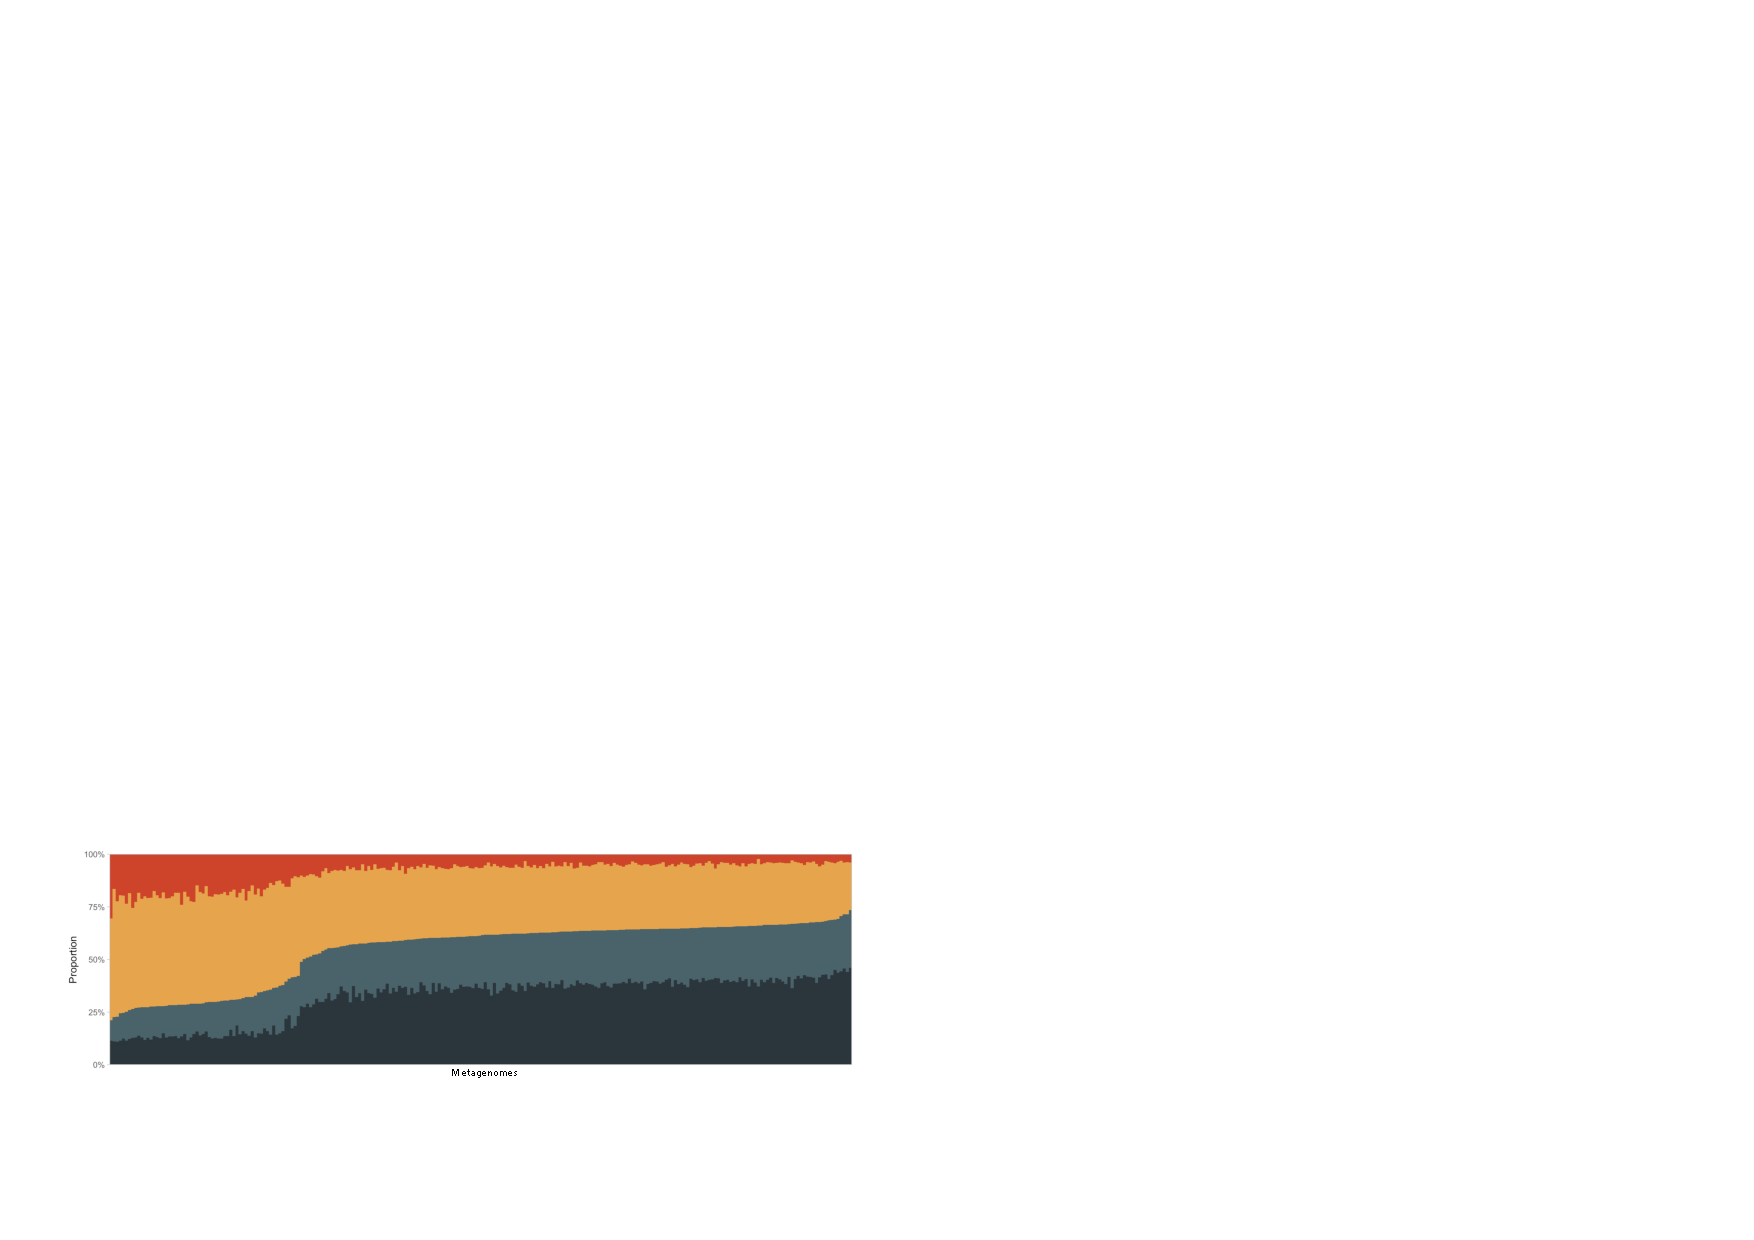
\includegraphics[width=1.0\textwidth] {fig_1.pdf}
	\caption[Proportions of Vanni et. al. cluster categories in the TARA Ocean metagenomes]{\textbf{Proportions of Vanni et. al. cluster categories in the TARA Ocean metagenomes.} The X axis denotes each of the TARA metagenomes while the Y axis is the relative proportion of the different Vanni et. al. cluster categories. Some of the metagenomes have greater than 70\% Unknowns. (Red = EUs; Yellow = GUs; Blue=Knowns; Black = Kwp)}\label{fig1}
\end{figure}

In 16S ribosomal DNA (rDNA) amplicon studies, amplified sequences are clustered together to form operational taxonomic units (OTU). This is advantageous because it reduces the data set for downstream computations and allows for annotation of the cluster representative with taxonomy. If each individual amplicon was treated as an OTU, alpha and beta diversity measurement computations would be very expensive thus making low resolution hypotheses about diversity difficult to make. A similar idea was applied by Vanni et. al. to their dataset to aggregate clusters into larger components due to the Known clusters exhibiting domain architecture redundancy. This may have been caused by the limitations of the clustering method used (based on sequence similarity) to detect distant homologies and the threshold selected (30\% of similarity), resulting in multiple clusters with the same domain architecture. \\

In total, there were 9,687 clusters with more than one PFAM annotation and 18,368 PFAM annotation combinations in the final clusters. To address this, they used the consensus sequence of the Knowns to create a sequence similarity network (SSN) and extracted components.\\

The term \quotes{components} will now be used for the rest of this thesis to describe aggregated clusters occurring in the TARA ocean dataset.\\

\textbf{Aim of this thesis}\\

The cluster components are ideal to address the main objective of this thesis - the exploration of the ecological significance and functional biogeography of the unknown functional diversity in the world\textquotesingle s oceans.\\

To echo back to the 16S rDNA amplicon analogy discussed previously, OTUs that do not receive a taxonomical annotation can still be included in ecological analyses. In this thesis, I use this philosophy but with unannotated ORF components. In the TARA Ocean data set, some samples have greater than 70\% of the metagenome categorized as unknown (Fig.~\ref{fig1}). Until now a large proportion of this functionally uncharacterized fraction has not been used for the study of the prokaryotic fraction \citep{Roux_2015}. In this thesis, it is demonstrate that including the whole metagenomic sample (Knowns and Unknowns) adds more variance to sample site ordinations. Also, it is shown that utilizing the unknowns in functional biogeography can lead to new insights into genetic differences between sites in different ocean regions. Finally, it is shown that there is a potential group of EU proteins that are ubiquitous throughout the ocean. To increase the evidence that the detected ubiquitous EUs are indeed real proteins in the environment, we localized them in the contigs (assembled sequence fragments from metagenomic data) of high quality, manually curated set of metagenomic assembled genomes (MAGs) extracted from the TARA ocean project \citep{Delmont_2017}. \\

% Methods

% Chapter Template

\chapter{Materials and Methods} % Main chapter title

\label{Methods} % Change X to a consecutive number; for referencing this chapter elsewhere, use \ref{ChapterX}

%\lhead{Chapter 1. \emph{Introduction}} % Change X to a consecutive number; this is for the header on each page - perhaps a shortened title

\renewcommand{\chaptermark}[1]{\markboth{#1}{}}
\renewcommand{\sectionmark}[1]{\markright{#1}}
\fancyhead[RE]{\small\leftmark}
% Section in the left on even pages}
\fancyhead[LO]{\small\rightmark}%Section in the left on odd pages

%\section{A section goes here}

\section{Initial dataset preparation}

The data used in this thesis was produced from the Vanni et. al. ORF clustering workflow (\url{https://orcid.org/0000-e2-1124-1147}) which includes The Human Microbiome Project (HMP), TARA Oceans, Ocean Sampling Day (OSD), Global Ocean Sampling Expedition (GOS), and Malaspina  (Table ~\ref{table:table1}). This dataset of 1,837 metagenomes (322,248,552 ORFs) was clustered into 32,465,074 total clusters, of which 2,953,903 were considered as high-quality. These high quality clusters were aggregated into components, then subsetted for only ones that occurred in the TARA prokaryotic enriched data set. This yielded a total of 18,644 components for the final data set used in this thesis (Table ~\ref{table:table2}).\\

\begin{table}[H]
\centering
\caption{Vanni et. al. initial clustering dataset}
\label{table:table1}
\begin{tabular}{@{}lcccc@{}}
\toprule
\textbf{Metagenomic Project} & \textbf{Number of Metagenomes} & \textbf{Number of ORFs} \\
\midrule
Human Microbiome Project & 1249 & 162,687,295 \\
TARA Oceans & 242 & 111,903,261 \\
Ocean Sampling Day & 150 & 7,015,383 \\
Global Ocean Sampling & 80 & 20,068,580 \\
Malaspina & 116 & 20,574,033 \\
\textbf{Total} & \textbf{1,837} & \textbf{322,248,522} \\
\bottomrule
\end{tabular}
\label{table:table1}
\end{table}

The TARA prokaryotic component abundance dataset (prokaryote-enriched fractions: 0.22 to 1.6 mm, 0.22 to 3 mm; n = 139) was filtered for low total count samples and low mean proportion components. Samples were removed from the analysis if their total component counts were less than the median total component count subtracted from  1.5 * MAD (Median Absolute Deviation) of the total counts. Next, components with a mean proportion less than 1e-5 across all samples were removed from the dataset using the Tidyverse package in R \citep{Wickham_2017}. The resulting filtered component abundance matrices were then stored as phyloseq objects \citep{Oksanen_2017, McMurdie_2013}. R version 3.4.3 (2017-11-30) was used for all R libraries mentioned in this thesis \citep{R}. \\

\begin{table}[H]
\centering
\caption{TARA subset of components used for this thesis}
\label{my-label}
\begin{tabular}{llllll}
\toprule
                    & \textbf{Knowns} & \textbf{GUs} & \textbf{EUs} & \textbf{Kwp} & \textbf{Total} \\
\midrule
\textbf{Components} & 3997            & 6497         & 1534         & 6616         & 18,644        \\
\bottomrule
\end{tabular}
\label{table:table2}
\end{table}

\section{Data standardization}

For PCA (principal component analysis) ordinations the dataset was center log ratio (CLR) transformed \citep{Piepel_1988} using the R bioconductor package, microbiome \citep{Lahti_2017}. Cumulative sum scaling (CSS) normalization from the R package metagenomeSEQ \citep{Paulson_2013} was applied to the dataset for the distance-decay analysis and nMDS (non-Metric Dimensional Scaling) ordinations.\\

\section{Indirect gradient analysis of TARA Ocean sample sites}

The CLR transformed, component abundance matrix was visualized using PCA. These calculations were performed using the R package Vegan \citep{Oksanen_2017} and graphically arranged using the R package ggpubr \citep{Kassambara_2017}. Sample sites in the ordinations were colored by sample depth category and the temperature to explore gradients and clustering patterns. Contextual data from the TARA Ocean project was used from \cite{Sunagawa_2015}.\\

Residuals of the PCA ordination were visualized to screen for normality and explore if the relationships between variables were linear. Additionally, a scree plot was plotted to visualize the variance captured by each principal component. Next, a NMDS plot was calculated, based on a Bray-Curtis dissimilarity matrix, to see if sample site clustering was similar to the PCA via a distance based ordination method. Additionally, a Shepard plot was visualized to explore how well the ordinated distances in the NMDS were a good representation of the actual distances within the dissimilarity matrix.\\

Hypotheses about the clustering results observed in the ordinations were tested for significance. This was done by calculating a PERMANOVA using the adonis function in the VEGAN package in R. Additionally, clustering due to beta-dispersion was explored by using the betadisper function, also in the Vegan package in R \citep{Oksanen_2017}.

\section{Niche breadth analysis of components}

To quantify scores of component theoretical niche and resource occupancy, Niche Breadth (B) was calculated \citep{Levins_1966}.\\

\[B = 1/\sum_{i=1}^{N}P^2ij \]

B is one divided by the sum of all proportions of a biological entity (P) from 1 to N sites of biological entity \textit{i}  through biological entity \textit{j}. From a macro-ecological perspective, B is one divided by the sum of all proportions a species represents in all the samples measured. The fact that P is squared in the denominator of the equation removes some additive effect of the summed proportions. 

To classify components as having a \quotes{wide} or \quotes{narrow}, a null distribution was created of each component B score. The original component abundance matrix was randomized 100 times using the Vegan package with the quasiswap count method in the function \textit{nullmodel} \citep{Mikls_2004, Oksanen_2017}. This method randomizes abundance matrices by mixing up numbers of 2x2 matrix subsets within the larger matrix. Additionally, the method maintains abundance matrix column and row sums to preserve original attributes of the matrix in the new randomized matrices. Once the distribution for each component is calculated, if a component score was in the top 2.5\% of its distribution, it was classified as \quotes{wide}. If it was in the bottom 2.5\% of the distribution, it was classified as \quotes{narrow}. The distributions of B categories were visualized using the R package ggplot2 \citep{Wickham_2016} and assembled using the R package ggpubr \citep{Kassambara_2017}.\\

\section{Screening beta diversity for geographic distance effects}

For this method section the CSS transformed, component abundance matrix was used. First, Bray-Curtis dissimilarity was calculated using the Vegan package function vegdist \citep{Oksanen_2017}. Distance-decay plots were determined by plotting the Haversine distance between TARA Ocean surface sample sites against the Bray-Curtis dissimilarities. Haversine distance was calculated using the R package geosphere \citep{Hijmans_2017}. The resulting graph was visualized using the R package ggplot2 (Wickham, 2016) and assembled using the R package ggpubr \citep{Kassambara_2017}. We used the function mantel and partial.mantel to test the correlation (spearman) between the Bray-Curtis dissimilarity and the geographic distance matrices. In the case of the partial Mantel test we use the deltaTemp matrix, the absolute temperature difference between TARA samples in degree Celsius. Mantel tests went through 9999 permutations.\\

TARA metagenomic sample sets defined by \cite{Delmont_2017} were used to separate TARA samples into three oceanic regions: Pacific, Atlantic, and Indian. In the Atlantic subset, samples were removed that were below the equator to focus analysis on the transect of the Gulf Stream. Distance-decay analysis was done separately for each region to remove biases of continental divides. Finally, component categories were separated into ubiquitous and non-ubiquitous. Ubiquitous components are defined as components that have a mean proportion greater than 1e-5 and be found in every sample in the TARA ocean project. To be categorized as non-ubiquitous, components only had to have a mean proportion greater than 1e-5.\\

\section{Analyzing the ubiquitous EUs}

The ubiquitous EUs were tested to see if they were real protein clusters and not artifacts of metagenomic sequencing or assembly. First, spurious proteins (falsely predicted ORFs) were filtered out by searching the EU clusters consensus sequence against the antiFAM database \citep{Eberhardt_2012} using the hmmsearch program from the HMMER suite \citep{Eddy_1998} with the \textit{--cut-ga} significance threshold. Results from the search were then parsed using e-value > 1e-5 and coverage >= 60\% as additional thresholds.\\

The second step to legitimize the ubiquitous EU clusters was to detect remote homology using an iterative HMM-HMM profile search of the EU clusters against the Uniclust database \citep{Mirdita_2016}. We used HHBlits from the HHsuite software package \citep{Remmert_2011} with two iterations. All queries with a probability larger than 90\% to any target sequence in the database were discarded. Next, we attempted to assign taxonomy to the remaining ubiquitous EUs by running Kaiju in greedy mode to ensure sensitivity and precision \citep{Menzel_2016}.\\

Finally, we mapped the ubiquitous EUs to high quality, manually curated MAGs from the TARA Ocean Project to see if they are found in populations of genomes \citep{Delmont_2017}. We aligned the cluster members from the ubiquitous EUs with FAMSA \citep{Deorowicz_2016} and we used the program hhmake from the HHSUITE to create hidden Markov model profiles (HMM). All EU HMM were stored, indexed, and retrieved using the file based storage software ffindex (\url{https://github.com/soedinglab/ffindex_soedinglab}, accessed 12.03.2018). EU HMM were retrieved and converted to MMSEQ2 format using \textit{convertprofiledb} from MMSEQS2. Next, the predicted ORFs of the TARA MAGs were converted to a MMSEQS2 database using the MMSEQS2 command \textit{createdb}. Finally, each ORF was mapped to the profile with the MMSEQS2 command search with the parameters \textit{-e} 1e-25, \textit--cov-mode 2 and -c 0.8. The results were then converted to a BLAST-tab formatted database using \textit{convertalis} program from MMSEQS2, then parsed and plotted with the ggplot2 package. Contigs containing the interesting ORFs were retrieved from the Anvi\textquotesingle o profiles using the program \textit{anvi-export-gene-calls} from Anvi\textquotesingle o v4 \citep{Eren_2015}. The functional annotation of the contigs was performed by Prokka \cite{Seemann_2014}  in metagenomic mode. The gene plots were drawn with the R package genoPlotR \citep{Guy_2010}. Muscle \citep{Edgar_2004} was used to create multiple sequence alignments of the components of interest, and the conserved consensus sequence logos were drawn using the WebLogo web server \citep{Crooks_2004}. Nucleotide sequences of the clusters with hits in the MAGs were also searched against NCBI nt and Microbial genomes using blastn from the BLAST package \cite{Camacho_2009}.\\

\section{Code and data availability}

All source code is available in a public repository. Additionally, all data used in this thesis will be available as FAIR data to ensure open science and access \citep{Wilkinson_2016}.\\

Github: \url{https://github.com/mschecht/Unknown_unknowns}

Figshare: DOI - 10.6084/m9.figshare.5979658

% Results and Discussion

% Chapter Template

\chapter{Results and Discussion} % Main chapter title

\label{Results and Discussion} % Change X to a consecutive number; for referencing this chapter elsewhere, use \ref{ChapterX}

%\lhead{Chapter 1. \emph{Introduction}} % Change X to a consecutive number; this is for the header on each page - perhaps a shortened title

\renewcommand{\chaptermark}[1]{\markboth{#1}{}}
\renewcommand{\sectionmark}[1]{\markright{#1}}
\fancyhead[RE]{\small\leftmark}
% Section in the left on even pages}
\fancyhead[LO]{\small\rightmark}%Section in the left on odd pages

%\section{A section goes here}

%A figure

\section{Balancing noise removal and sparsity of component abundance dataset}

The ecological analyses in this thesis started with two datasets of component counts from the TARA ocean prokaryotic metagenomes from all depths (TP) and only the surface samples (TPS). These two datasets were filtered first for low total count samples and second for low mean proportion components (Methods 2.1). This ensured that: (1) extremely low abundant components were filtered out; (2) sequencing noise was removed; and (3) overall size of the resulting abundance matrices was decreased to lower computational resources for calculations.

\begin{figure}[h!]
	\centering
	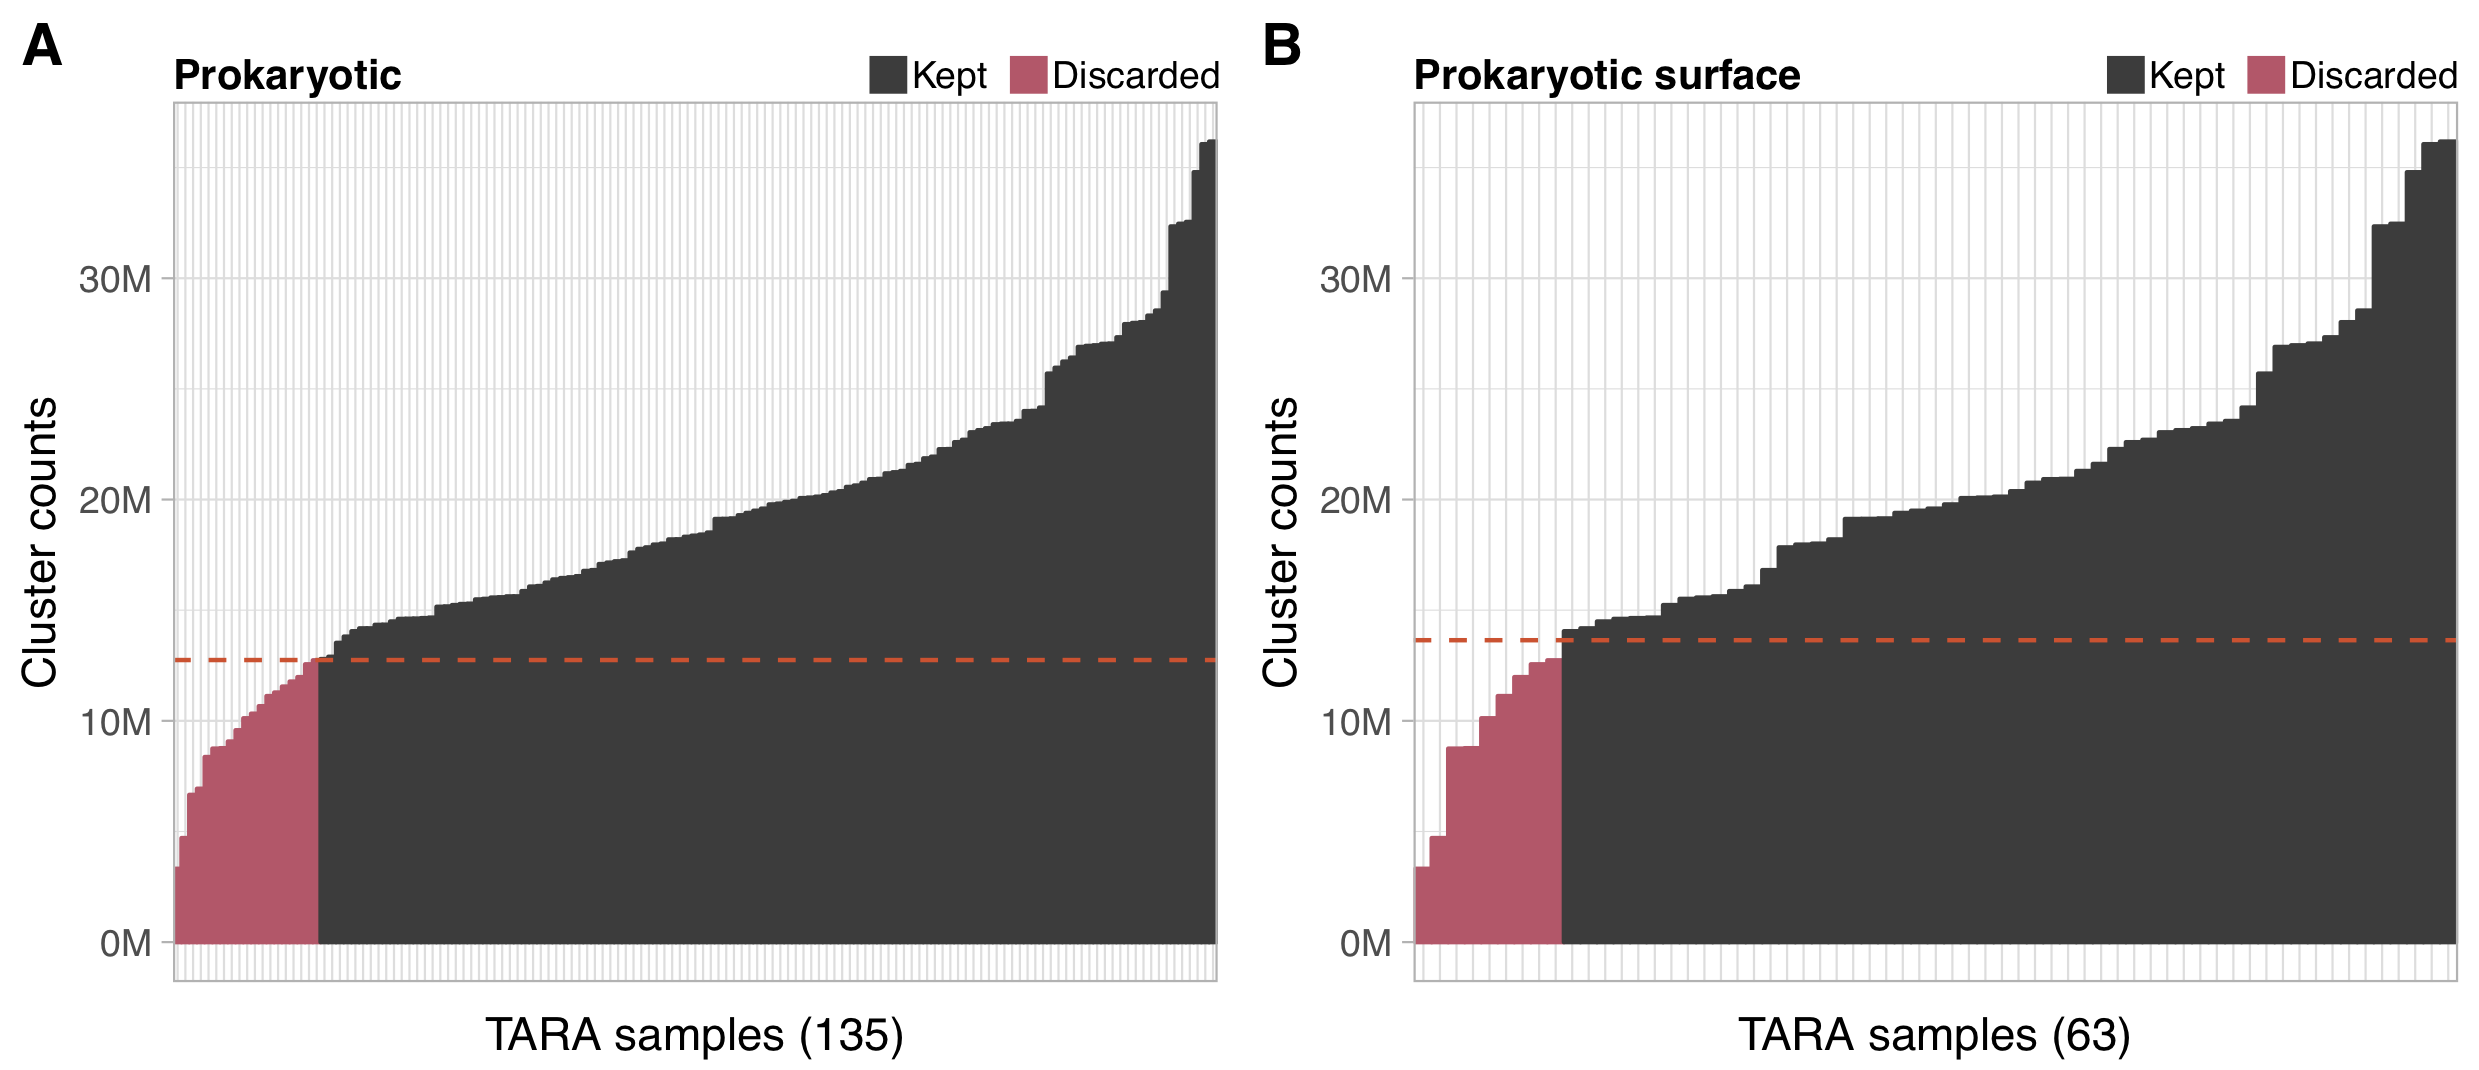
\includegraphics[width=1.0\textwidth] {fig_2}
	\caption[Step 1 of dataset filtering - removing low count samples]{\textbf{Step 1 of dataset filtering - removing low count samples.} X axis denotes each sample in the dataset while the Y axis denotes total cluster counts for each sample. Samples with total counts below the value, median subtracted from 1.5*MAD, were removed from the analyses. (A) Total component counts for TARA prokaryotic metagenomes (TP). (B) Total component counts for TARA surface, prokaryotic metagenomes (TPS).}
	\label{fig:fig2}
\end{figure}

During the first filtering step, nine samples were removed from the TPS dataset and 19 samples were removed from TP dataset. Sample with low total counts, relative to other samples, have the potential to distort beta-diversity analysis because their total counts could make them more similar to each other due to low counts rather a real beta-diversity signal. The cutoff threshold, Median - 1.5*MAD, was chosen because the MAD statistic was chosen it is a reliable measurement of the center of the data and is not sensitive to outliers (Figure~\ref{fig:fig2}). \\

The second filtering step removed all components that had a mean proportion across all samples lower than 1e-5. After this step, the final TPS dataset contained 18,644 components while the TP dataset contained 15,353 respectively. This was an effective cutoff for both the TP and TPS datasets because overall component content and counts were able to be maximized while sparsity was lowered. The less sparsity an abundance table has, the more power the abundance variables have in explaining the dataset. Yet, a side effect of decreasing sparsity is removing counts which decreases the total amount of information the dataset has. In both datasets, if the mean proportion requirement was increased to 1e-4, sparsity would have reached close to 0. This could have led to a large amount of total counts and components being sacrificed. For this analysis, we did not want to remove the low abundance signals in order to capture more functional diversity in the dataset. A summary of the 1e-5 mean proportion plot against sparsity, total counts, and proportions can be seen in Figure~\ref{fig:fig3}. \\

\begin{figure}[h!]
	\centering
	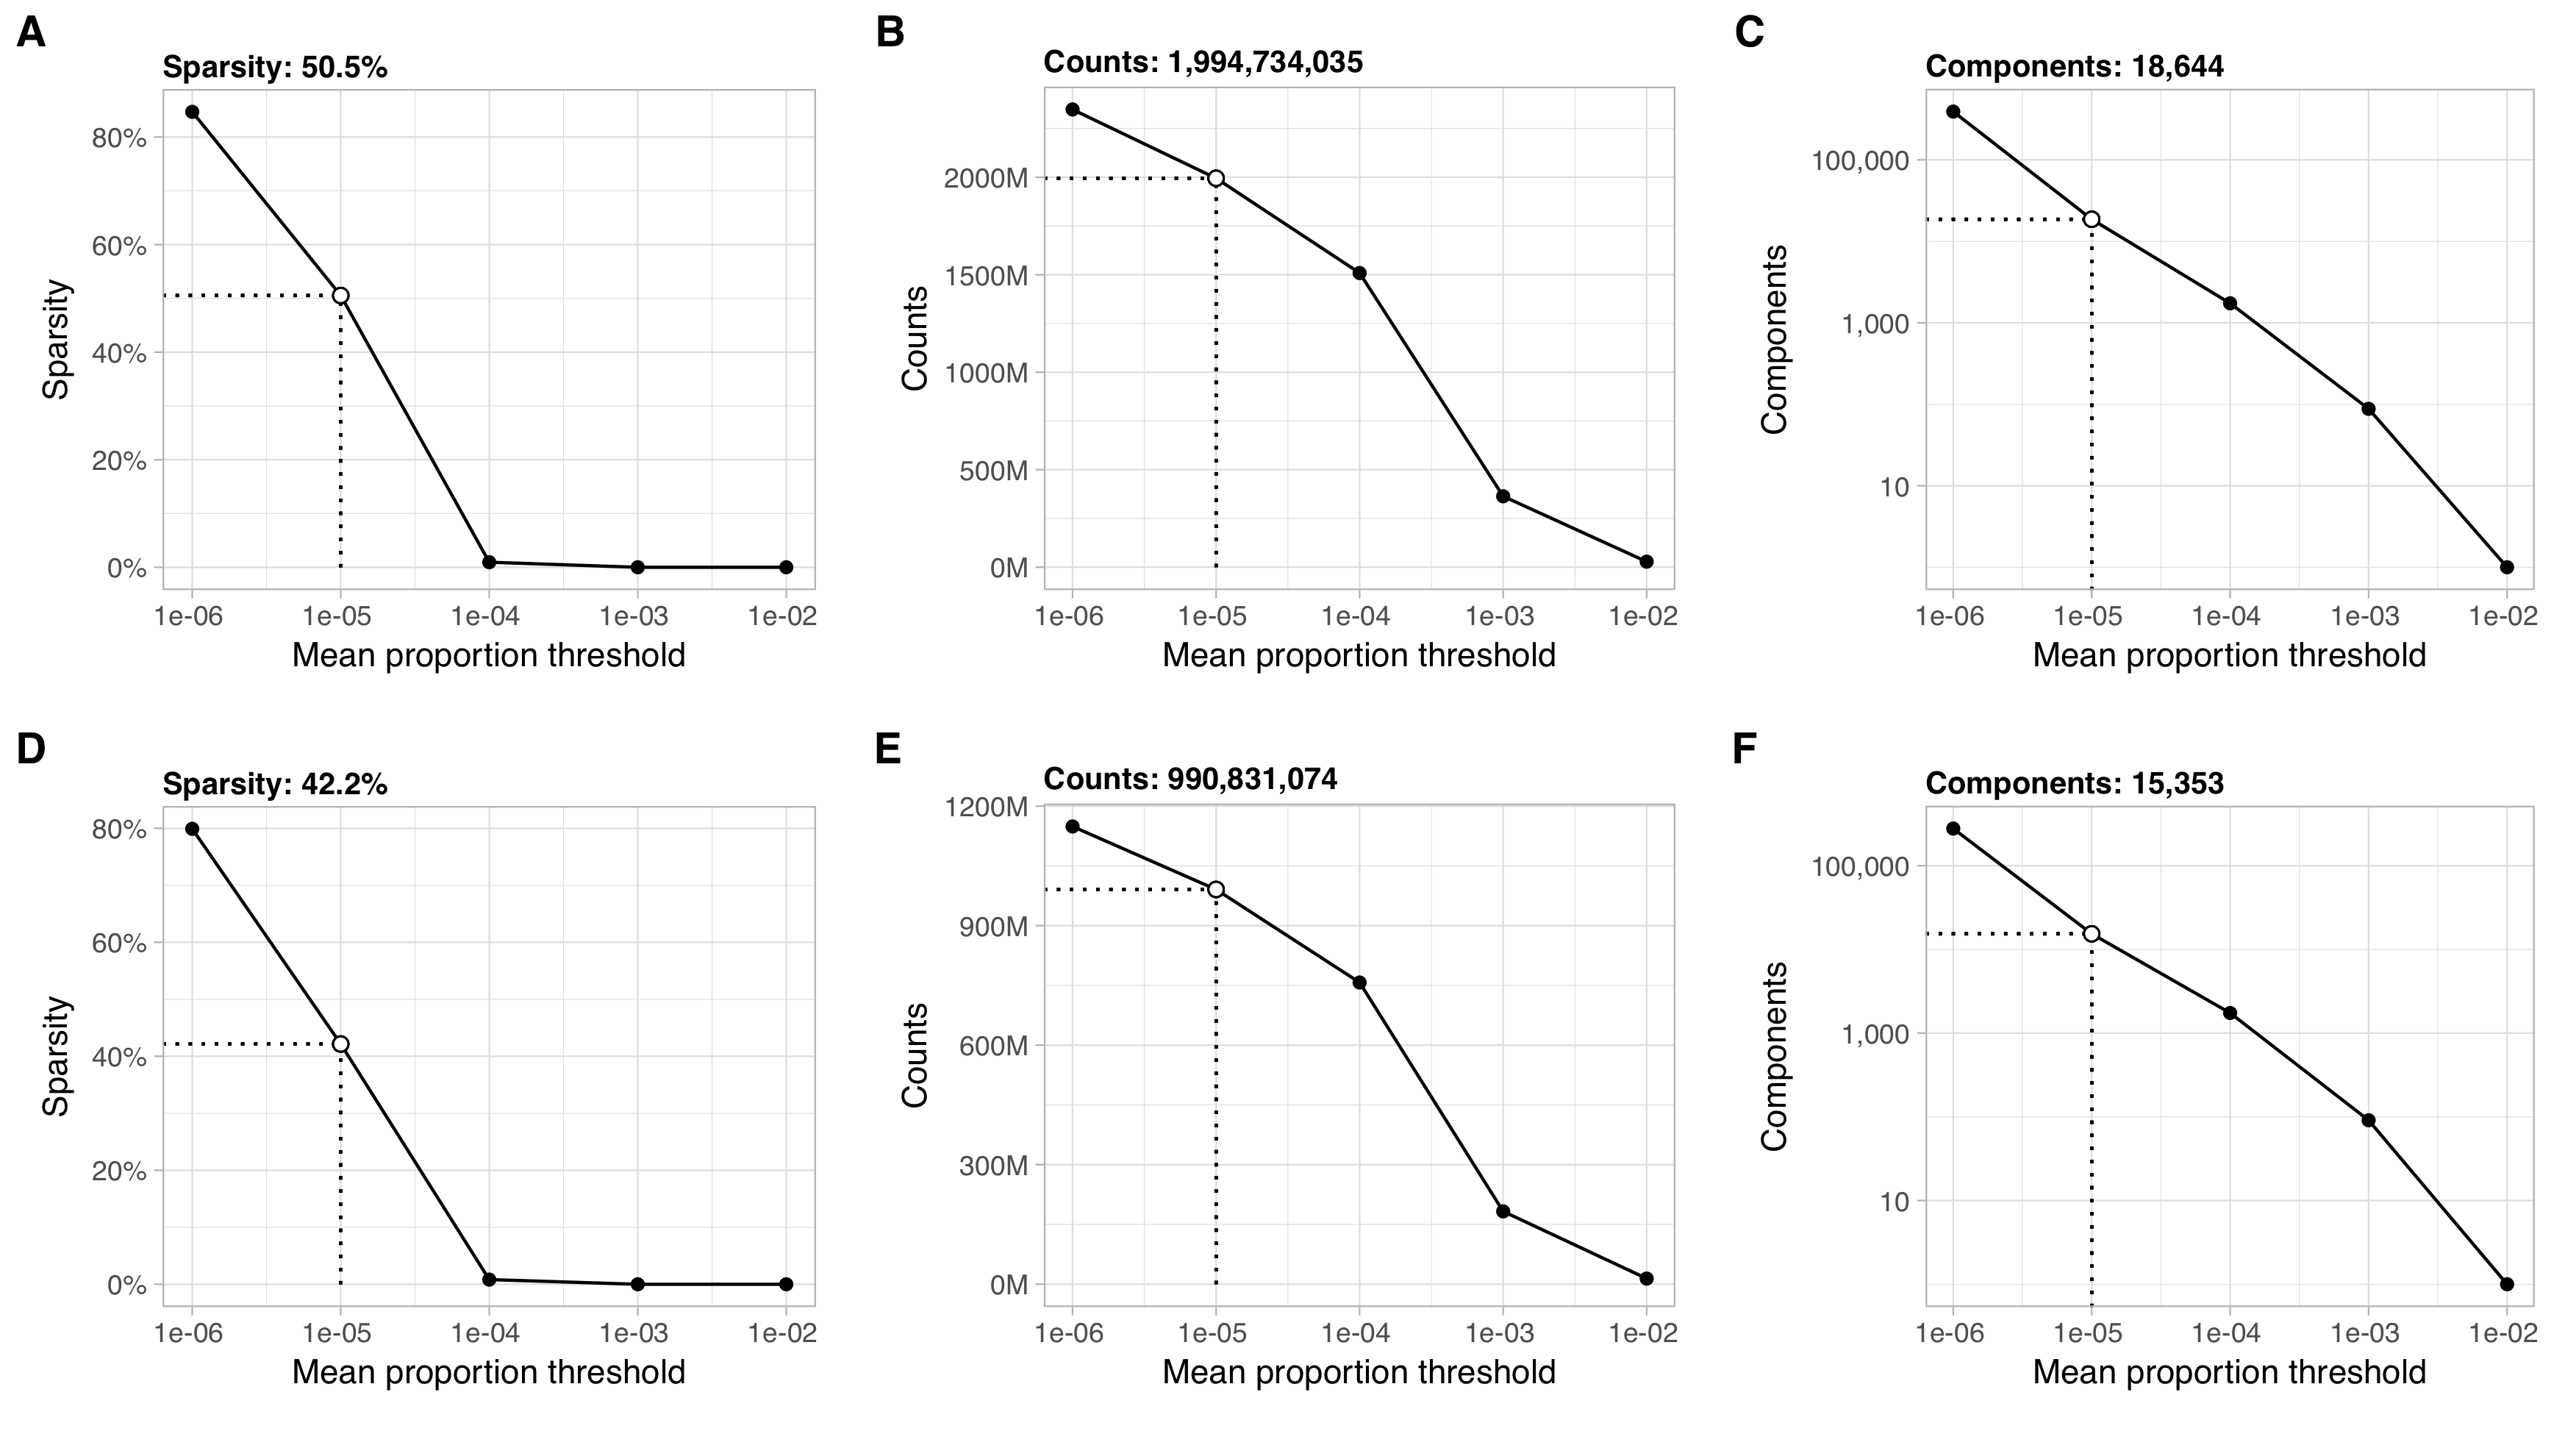
\includegraphics[width=1.0\textwidth] {fig_3}
	\caption[Step 2 of dataset filtering - removing low abundance components]{\textbf{Step 2 of dataset filtering - removing low abundance components.} Metagenome component mean proportion (1e-5 cutoff) is plotted against dataset sparsity, total cluster counts, and number of components.  A-C represent the TARA prokaryotic, all depths dataset (TP). D-F represent the TARA prokaryotic, surface dataset (TPS).}
	\label{fig:fig3}
\end{figure}

\section{Indirect gradient analysis of TARA Ocean sites based on component abundances}

\begin{figure}[h!]
	\centering
	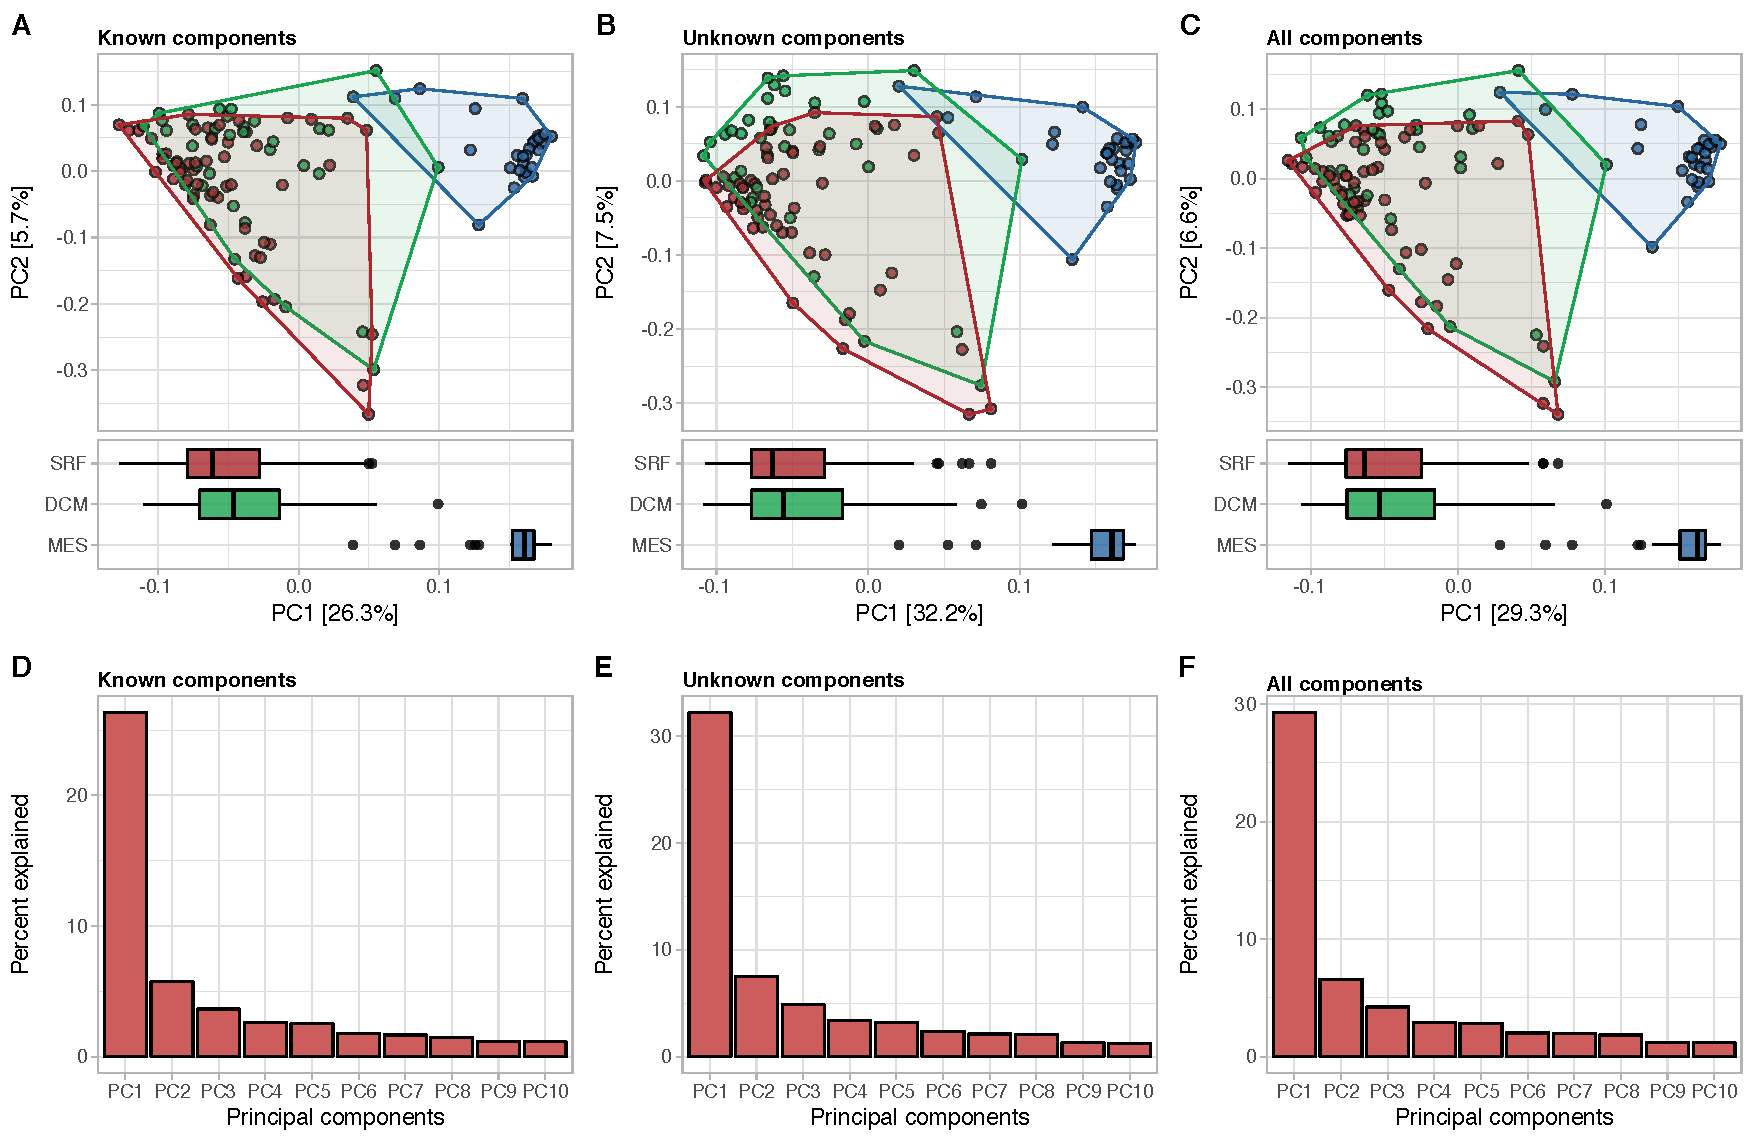
\includegraphics[width=1.0\textwidth] {fig_4}
	\caption[Principal component analysis (PCA) of 135 TARA Ocean prokaryotic metagenome sampling sites from surface (SRF), deep chlorophyll maximum (DCM), and mesopelagic (MES) sites]{\textbf{Principal component analysis (PCA) of 135 TARA Ocean prokaryotic metagenome sampling sites from surface (SRF), deep chlorophyll maximum (DCM), and mesopelagic (MES) sites.} A-C) Sites are colored by depth of origin and are defined by proportions of component categories: Unknowns (EU + GU), Knowns (K + Kwp), All (EU + GU + K + Kwp). Below each ordination are bar plots of the distribution of each depth category across the first principal component axis. D-F) Scree plots of each PCA. The X axis denotes each principal axis while the Y axis denotes the percent variance explained by the axis. Residuals of each PCA ordination can be found in the Appendix~\ref{Fig:A2}}
	\label{Fig:fig4}
\end{figure}

Principal component analysis (PCA) of the TARA ocean prokaryotic sample sites produced a meaningful ordination (Figure~\ref{Fig:fig4} A-C). Due to the effect of compositionality often associated with omics datasets, a center log ratio transformation (CLR) was performed prior to calculated the PCA \citep{Gloor_2017}. Scree plots indicated that in all three ordinations the majority of variance was captured in the first two principal component axes (PC) (Figure~\ref{Fig:fig4} D-F). Additionally, histograms of residuals were calculated and showed a bimodal distribution around 0 (Appendix~\ref{Fig:A1}). NMDS ordination was calculated using pairwise site Bray-Curtis dissimilarity (Appendix~\ref{Fig:A2}). The calculation was iterated 20 times with a stress around 0.8 for all categories (Table~\ref{table:3.1}). \\

\begin{table}[]
\centering
\caption{Stress Values for NMDS ordination}
\label{table:3.1}
\begin{tabular}{@{}lc@{}}
\cmidrule[\heavyrulewidth](l){2-2}
                     & \textbf{NMDS stress} \\ \midrule
\textbf{Unknowns (EUs + GUs)} & 0.07997218           \\
\textbf{Knowns (K + Kwp)}     & 0.08218745           \\
\textbf{All combined}         & 0.07974366           \\ \bottomrule
\end{tabular}
\end{table}

\section{TARA Ocean Sites cluster based on depth}

PCA ordinations of the TARA ocean prokaryotic sample sites clustered based on their depth of origin (surface (SRF), deep chlorophyll maximum (DCM), and mesopelagic (MES) regardless of which component category sites are defined by. The SRF and DCM sites overlap, while the MES samples form their own cluster. Additionally, in all cases the first principal component axis (PC1) explains the most variance in the ordination. PERMANOVA of the ordination against the depth categories and temperature from the associated metadata was significant, allowing the rejection of the null hypothesis that the three depth categories have the same cluster centroids in the ordination (Table~\ref{table:3.2}). Additionally, beta-dispersion was not significant in terms of the depth category (Table~\ref{table:3.2}) and indicates that clustering was not due to dispersive effects. If beta-dispersion was significant, it would indicate that clustering of sites in the ordination was due to dispersion effects of the data and not entirely due to depth category. But since it was not significant, there is increased confidence in the PERMANOVA results. NMDS ordination based on Bray-Curtis dissimilarity also show the same clustering of sites based on depth category and temperature (Appendix~\ref{Fig:A2}). \\

Previous ordinations of the TARA Ocean metagenomes have shown site clustering by depth of origin \citep{Sunagawa_2015, Louca_2016}. \cite{Louca_2016}, calculated a metric multidimensional scaling (MDS) of the TARA sampling sites, but instead, defined sites based on aggregated, biogeochemically relevant microbial functions. Additionally, \cite{Sunagawa_2015} and \cite{Louca_2016} calculated a principal coordinate analysis with sites defined by 16S rDNA gene tags (miTAG) extracted from the metagenomes. Both analyses concluded that prominent environmental factors (e.g. temperature, nutrients levels, access to light) from the different depth layers have a strong influence in shaping the structure and function of the microbial community. This explanation can be applied to this analysis as well.\\

\begin{table}[]
\centering
\caption{TARA ocean prokaryotic metagenome sampling site ordination PERMANOVA for depth category hypothesis testing}
\label{table:3.2}
\begin{tabular}{@{}lcccc@{}}
\cmidrule[\heavyrulewidth](l){2-4}
                              & \multicolumn{2}{c}{PERMANOVA}  & \multicolumn{1}{c}{Beta-dispersion} \\ \cmidrule(l){2-4}
                              & {$\bm{R^2}$} & \textbf{p-value}    & \textbf{p-value}    \\ \midrule
\textbf{Unknowns (EUs + GUs)} & 0.27237         & 0.001            & 0.073                            \\
\textbf{Knowns (K + Kwp)}     & 0.22649         & 0.001            & 0.121                            \\
\textbf{All combined}         & 0.25064         & 0.001            & 0.117                            \\ \bottomrule
\end{tabular}
\end{table}

Regardless of what cluster categories ORFs are from, the environmental factors from the depth layer are selecting components in a similar way. The SRF and DCM samples may overlap due to depth proximity. Both SRF and DCM are sunlit environments and have access to fresh primary production carbon sources. On the other hand, the MES samples clusters separately from the SRF and DCM. This is most likely owing to the different environmental factors in the MES, such as lack of solar radiation, lower temperatures, and higher dissolved oxygen and nutrients, which can select for different microbial functions than the epipelagic depths. Additionally, there is increased amounts of recalcitrant carbon sources in the MES because smaller/simple carbohydrate sources are most likely respired at high depths of the biological carbon pump \citep{Azam_2007}. In an environment with more complex carbon sources, a diverse array of microbial functions may be selected for to metabolize a wider range of nutrients.\\

\section{Greater variance observed in PCAs when all components are used to define sample sites}

In Figure~\ref{Fig:fig4} A-C, more variance is captured in PC1 of the Unknowns (32.2\%) while less variance is captured in the Knowns PC1 (26.3\%). The Knowns + Unknowns PC1 variance falls in between (29.3\%). The fact that PC1 of the Unknowns ordination has the most variance infers that sites are more dissimilar when they are defined by the unknown fraction of components. Also, by accounting for both the Known and Unknown fraction in the All ordination, the site dissimilarity is effectively increasing by including the Unknown fraction.
Similar to defining sites with all detected OTUs regardless if taxonomy is assigned to them, ORF clusters, with or without annotation, can be tracked as a functional entity in metagenomes and help separate samples in higher resolution. Louca et al., 2016 ordinated the TARA Ocean sites based on biogeochemical relevant microbial functions and determined there was functional redundancy in the ocean. This conclusion may have been constrained by the fact that sites were only defined by known functions. If the Louca et al., 2016 sites were defined with the complete functional repertoire of the metagenomic sample, their results may have had increased dissimilarity. It is clear that when sites are defined by the knowns and the unknowns, more variance is added to the ordination. This may indicate that the unknown fraction could be site specific adaptive proteins. \\

\section{Unique component composition in Southern Ocean Samples}

\begin{figure}[h!]
	\centering
	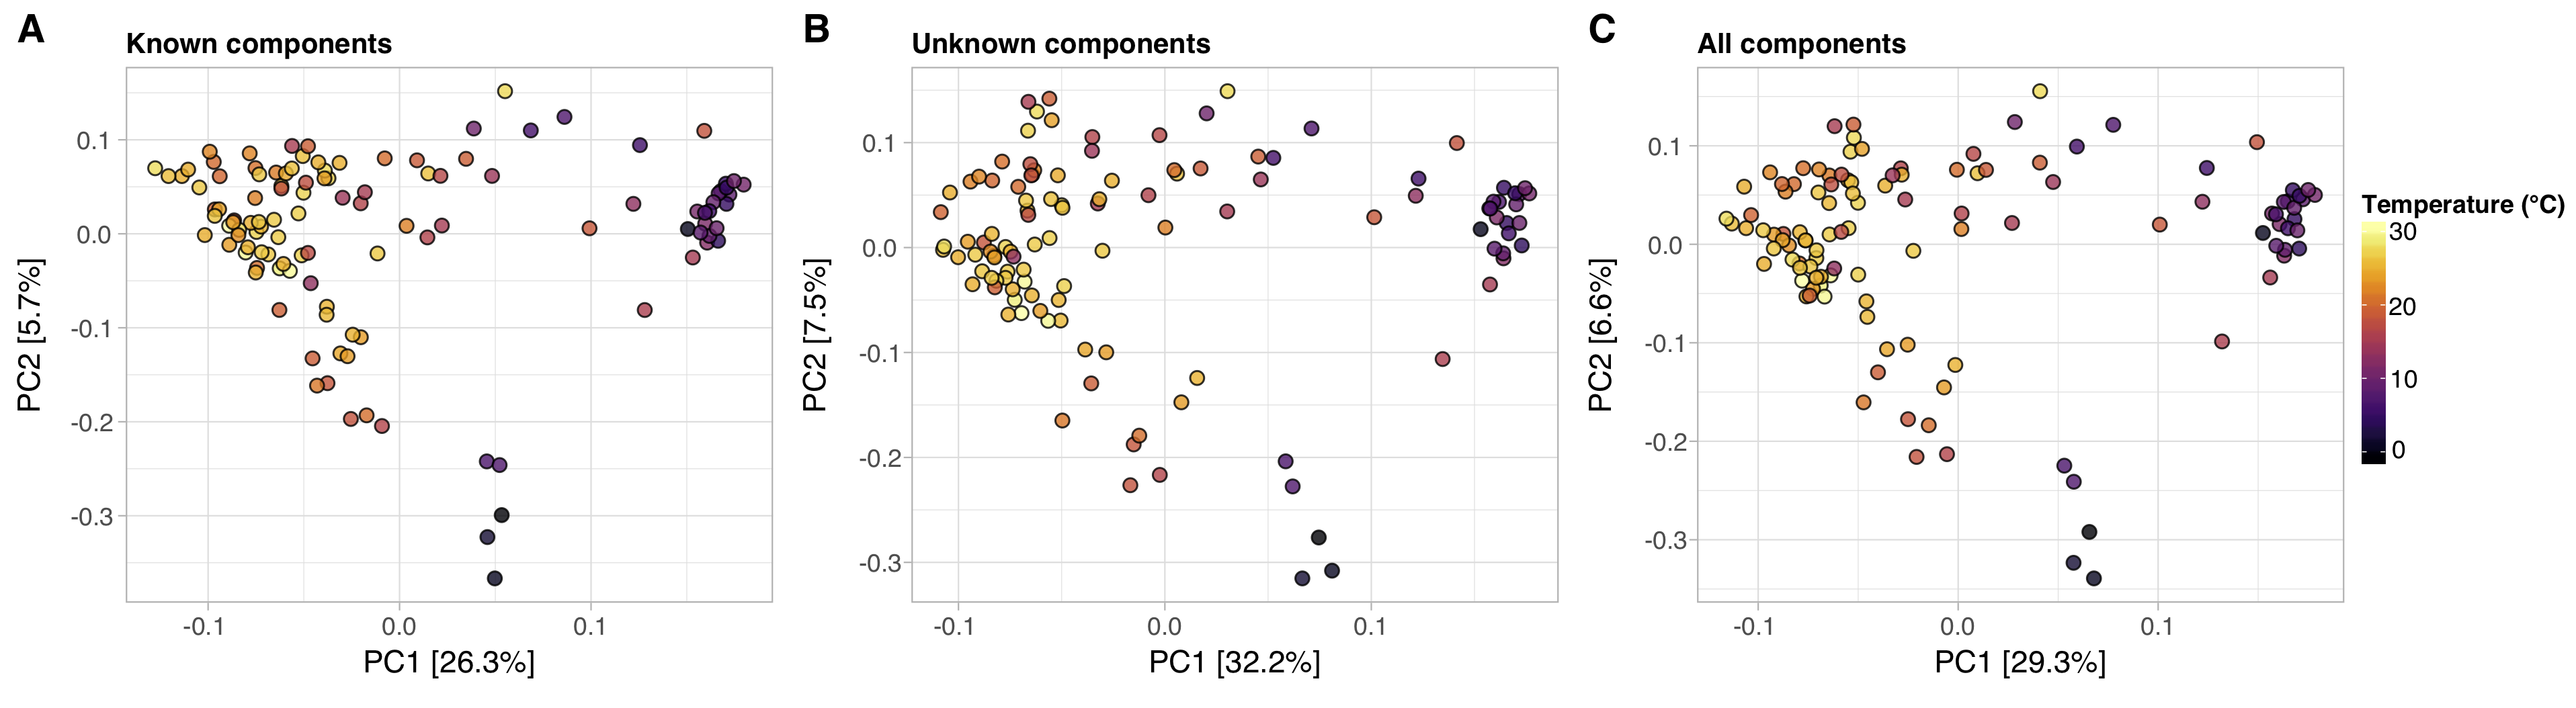
\includegraphics[width=1.0\textwidth] {fig_5}
	\caption[Principal component analysis of the prokaryotic fraction of the 139 TARA ocean sampling sites from all depths colored by temperature]{\textbf{Principal component analysis of the prokaryotic fraction of the 139 TARA ocean sampling sites from all depths colored by temperature.} Sites are defined by proportions of component categories: Unknowns (EU + GU), Knowns (K + Kwp), All (EU + GU + K + Kwp)}
	\label{Fig:fig5}
\end{figure}

A temperature gradient across PC1 of Figure~\ref{Fig:fig5} was ordinated in the TARA sampling sites. Samples in the SRF and DCM cluster have warmer temperatures while the MES cluster has the coldest temperatures. Colder samples from the SRF and DCM ordinate closer to the MES cluster. These results are in line with Sunagawa et al., 2015 who found that temperature is the main driving factor for community composition in the ocean. The SRF and DCM have warmer temperatures due to increased solar radiation, while heat is dissipated in the MES. The clustering of the ordinations based on the origin depth of the sample may be due to temperature which could then select for different microbial functions (PERMANOVA for temperature found in Table~\ref{table:3.3}). \\


\begin{table}[]
\centering
\caption{TARA ocean prokaryotic metagenome sampling site ordination PEMANOVA for temperature hypothesis testing}
\label{table:3.3}
\begin{tabular}{@{}lcccc@{}}
\cmidrule[\heavyrulewidth](l){2-3}
                              & \multicolumn{2}{c}{PERMANOVA}  \\ \cmidrule(l){2-3}
                              & {$\bm{R^2}$} & \textbf{p-value}        \\ \midrule
\textbf{Unknowns (EUs + GUs)} & 0.27237         & 0.001                                     \\
\textbf{Knowns (K + Kwp)}     & 0.22649         & 0.001                                    \\
\textbf{All combined}         & 0.25064         & 0.001                                       \\ \bottomrule
\end{tabular}
\end{table}


%\begin{table}[]
%\centering
%\caption{TARA ocean prokaryotic metagenome sampling site ordination PEMANOVA for temperature hypothesis testing}
%\begin{tabular}{lll}
%\toprule
%\textbf{Component Category}   & \textbf{PERMANOVA $R^2$} & \textbf{p-value} \\
%\midrule
%\textbf{Unknowns (EUs + GUs)} & 0.21144                                & 0.001            \\
%\textbf{Knowns (K + Kwp)}     & 0.17109                                & 0.001            \\
%\textbf{All combined}         & 0.19232                                & 0.001           \\
%\bottomrule
%\end{tabular}
%\label{table:3.2}
%\end{table}

An exception to the temperature gradient across PC1 is the three Southern Ocean samples (TARA site 84 SRF, DCM and site 85 SRF) at the bottom of the ordination. Even though they are some of the coldest samples in the dataset, they do not follow the temperature gradient along PC1 and do not cluster with the rest of the cold MES samples. In fact, PC2 appears to drive their separation from the rest of the samples. \\

These three Southern Ocean samples may have a unique component composition due to their placement in the Antarctic Circumpolar Current (ACC). The ACC is a located in the Southern Ocean and presents a unique biome compared to other oceanic currents due to its strength, isolation, dramatic seasonal light flux and nutrient levels. Strong westerly winds around Antarctica drive the current due to pressure gradients caused by surface wind friction and density differences. Because no continents obstruct its flow, the ACC is the only ocean current system that circles the earth on a similar latitude range. This allows to be the fastest current in the ocean with speeds around 130e6 $\frac{m^3}{s^-1}$ through Drake passage (MarMic Physical Oceanography Lecture, 2017).\\

The ACC also has unique physicochemical properties that may also influence specialized microbial functions. Due to low altitude wind cells, Aeolian dust input is limited which makes mineral concentrations limited. On the other hand, strong upwelling increases concentrations of other nutrients, such as nitrate and phosphate. This makes for a unique environment because despite high nutrients, chlorophyll levels are low due to Fe limitations \citep{Martin_1990, Tagliabue_2014, Cavicchioli_2015}. Additionally, the ACC has unique biogeography due to dramatic polar light cycles. During summer season, long periods of light generate high levels of primary production, while during low light winter's, the overall microbial community switches to different ecological strategies such as heterotrophy and predation \citep{Wilkins_2013, Milici_2017}. Due to the reasons listed above, unique functions for local adaptation in the Southern ocean may be driving the dissimilarity from the other TARA ocean samples.\\

Interestingly, TARA site 85 MES metagenome did not cluster with the Antarctic SRF and DCM metagenomes at the bottom of the ordination, but rather clustered with the rest of the MES metagenomes. This reinforces that the MES is a different environment compared to the SRF and DCM. Even though TARA site 85 MES was sampled in the ACC, the deep depth layer environmental parameters have a stronger influence on its component composition. To further explore this observation, direct gradient analysis should be applied to the Southern Ocean to resolve its unique microbial functional properties.\\

Using sites to ordinate the TARA ocean sites revealed a distinct functional difference between the Southern Ocean samples and the rest of the TARA samples. This was in part due to the use of components to define sites. No matter which category of components was used (Knowns, Unknowns, All), the Southern Ocean samples we separated. This is an indication that defining sites based off of component composition may help resolve fine differences between sites in ecological analyses in the future. \\

The ordination of sample sites based on the different component fractions preliminarily indicated that the Unknown fraction may be able to increase site dissimilarity. To investigate further, we performed a Levin\textquotesingle s Niche Breadth analysis to explore component niche occupancy.\\

\section{Niche Breadth analysis of component distribution}

According to \cite{Levins_1966}, Niche breadth (B) is the theoretical, multidimensional range of resources and habitats a species can occupy and access. Here we used the equation 1 to quantify the niche specialization of all prokaryotic components in the TARA oceans sampling sites. B was originally designed to classify macro-ecology abundance biogeography, i.e. birds and deer in different environments. Ocean microbial systems are different compared to  macro-ecological systems for a few reasons. First, the definition of species in microbial ecology is still debate. Second, microbes are subjected to functional and physiological plasticity due to horizontal gene transfer. With these factors in mind, the Niche Breadth measurement may still be informative for analyzing the distribution of components. Recently, the measurement was used to describe the biogeography of operational taxonomic units (OTUs) in coastal Antarctic lakes \citep{Logares_2012}. \cite{Logares_2012} used B to denote \quotes{generalists} vs \quotes{specialists} to explore niche specialization of microbes within the domain of the sampling regime. It has also been hinted that the distributions and associations of genes with ecological niches may be an effective strategy for determining the role of accessory/adaptive genes in pangenomic diversity \citep{Shapiro_2017}. Although more research needs to be done, these studies have laid groundwork for using Niche Breadth in the context of component distribution. \\

\begin{figure}[h!]
	\centering
	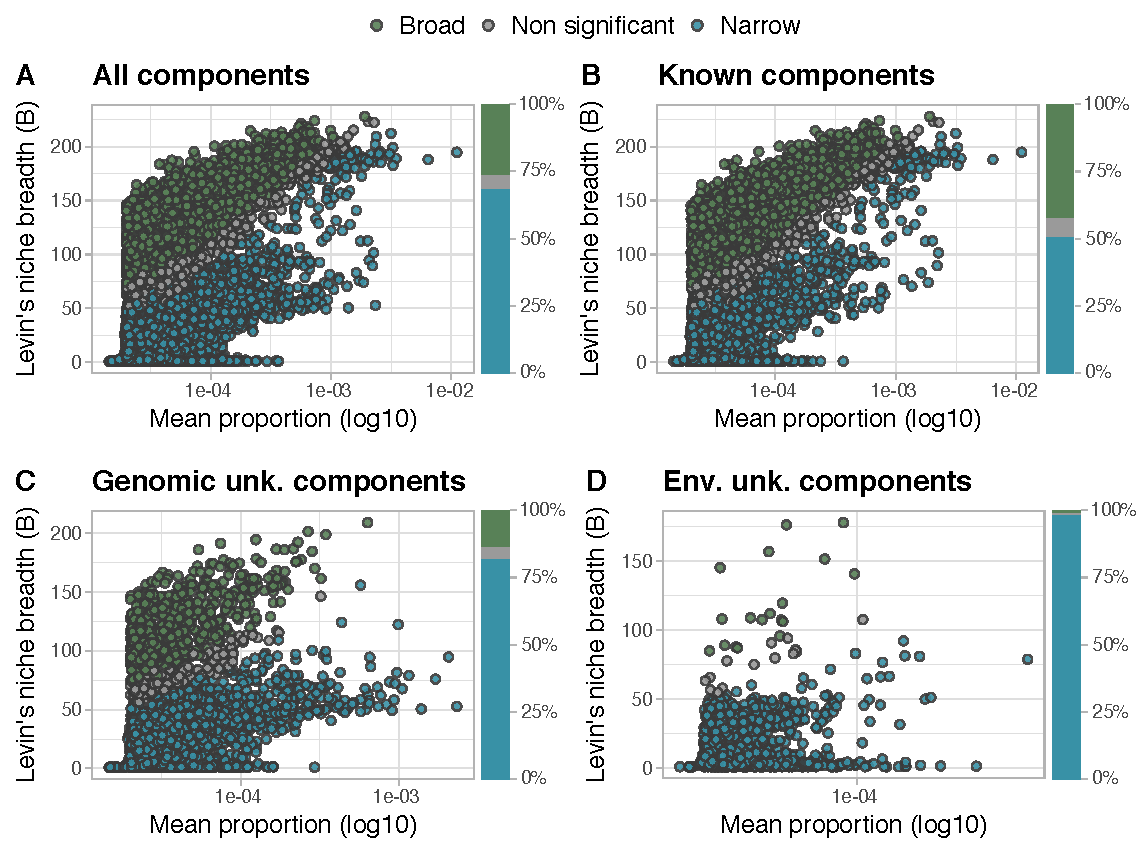
\includegraphics[width=1.0\textwidth] {fig_6}
	\caption[Levin\textquotesingle s Niche Breadth (B) scores of the component categories]{\textbf{Levin\textquotesingle s Niche Breadth (B) scores of the component categories.} The x-axis denotes the average, relative abundance of a component across all TARA prokaryotic metagenomes. The y-axis denotes a component B scores. Components are colored by their classification due to their B score. The bar charts on the right of each plot represent the relative proportions each B classification in the component category. See section 2.4 for description of classification of the components based off their B score.}
	\label{Fig:fig6}
\end{figure}

This niche breadth analysis revealed that greater than 99\% of the EU components have a narrow niche breadth. Also, the majority of GUs are narrow while the Knowns are more evenly distributed between narrow and wide components. In the sample site ordination, it was found that including the Unknown fraction increases variance between sites. This result compliments the Niche Breadth analysis because the majority of the GU and EU components are categorized as having a narrow B (i.e. found in a few samples in higher proportions). EUs in general being associated with narrowness may indicate that they are selected in prokaryotic genomes due to specific environmental factors that occur in niche spaces (TARA ocean sampling sites). These components may be uncharacterized EUs because they are non-core, accessory functions from members of the rare biosphere \citep{McInerney_2017}. Functions from the rare biosphere are difficult to characterize due the inability to culture members and assemble their genomes into metagenomic assembled genomes due to low read coverage. \\

In Figure~\ref{Fig:fig6} D, there is a group of EU components that are narrow and with mean proportions greater than 1e-4. This indicates that they are found in relatively high abundance in only a few samples. These components may be truly adaptive and could be providing the microbes with a selective advantage. Additionally, in Figure~\ref{Fig:fig6} B and C, there are Known and GU narrow components with mean proportions greater than 1e-3. These components may also be adaptive components and could be immediately investigated due the Knowns having a Pfam annotation and the GUs being associated with taxonomy.\\

Though taxonomy and functional annotations are not available for the EUs by definition, the niche breadth analysis still provides more evidence that they are environmentally adaptive proteins in microbes that have be selected for by specific niche factors at the site. To increase evidence for this hypothesis we examined the component categories from a biogeographical point of view. \\

\section{Beta diversity analyses}

Microbial beta-diversity was explored in relation to geographical distance between sampling sites. The general hypothesis for this analysis is that sites will increase in genetic dissimilarity (beta-diversity) with increasing distance. Here we perform a distance-decay analysis while defining beta diversity by different component categories: Unknowns (EU + GU), Knowns (K + Kwp), and All (Known + Unknown). \\

The results of distance-decay analysis of the TARA ocean surface, prokaryotic metagenomes samples shows that beta-diversity between sites is the most dissimilar when sites are defined by the Unknowns in all three ocean regions (Figure~\ref{Fig:fig7} B, E). When sites are defined by the Known fraction, they are the most similar (Figure~\ref{Fig:fig7} D). It is also shown that when the Unknown fraction is included with the Known fraction that overall dissimilarity between sites is increased (Figure~\ref{Fig:fig7} B). \\

The fact that sites are more dissimilar when defined by the Unknowns is another indication that the Unknown fraction may represent proteins specific to niche adaptation of particular sites. The environments at each sample site may have a unique signature of adaptive proteins and thus increase overall site dissimilarity. Another aspect to consider is the Unknown fraction is around 33\% of all clusters in this analysis. Because the abundance matrix of a site, when defined by the Unknowns, will always be smaller than then Known abundance matrix (due to the proportions of the component categories), the Unknowns matrix may be more sensitive to unique site abundance signals, thus increasing beta dissimilarity.\\

\begin{figure}[h!]
	\centering
	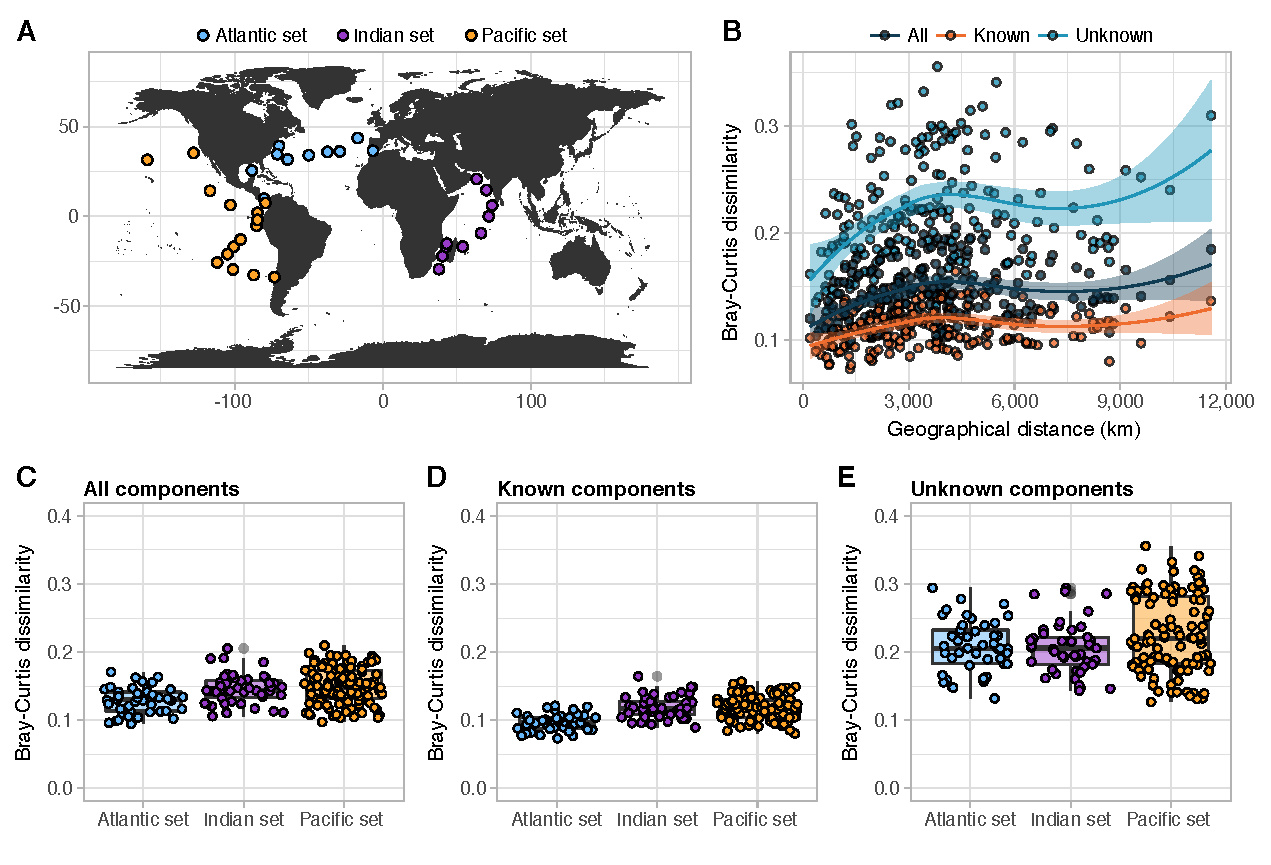
\includegraphics[width=1.0\textwidth] {fig_7}
	\caption[Sample sites beta-diversity vs. geographic distance]{\textbf{Sample sites beta-diversity vs. geographic distance.} A) Map of TARA Ocean samples used for distance-decay analysis. Samples were divided into regions: Pacific, Atlantic, and Indian. B) Combined distance-decay of samples between all regions. Sites appear three times defined by the Unknowns (EU + GU), Knowns (K + Kwp), and All. The x-axis denotes the geographical distance between sampling sites, while the y-axis denotes the Bray-Curtis dissimilarity beta diversity measurement. (C-E) Box-plots of the pairwise Bray-Curtis dissimilarity beta diversity measurement for each component category, separated by ocean region.}
	\label{Fig:fig7}
\end{figure}

\begin{figure}[h!]
	\centering
	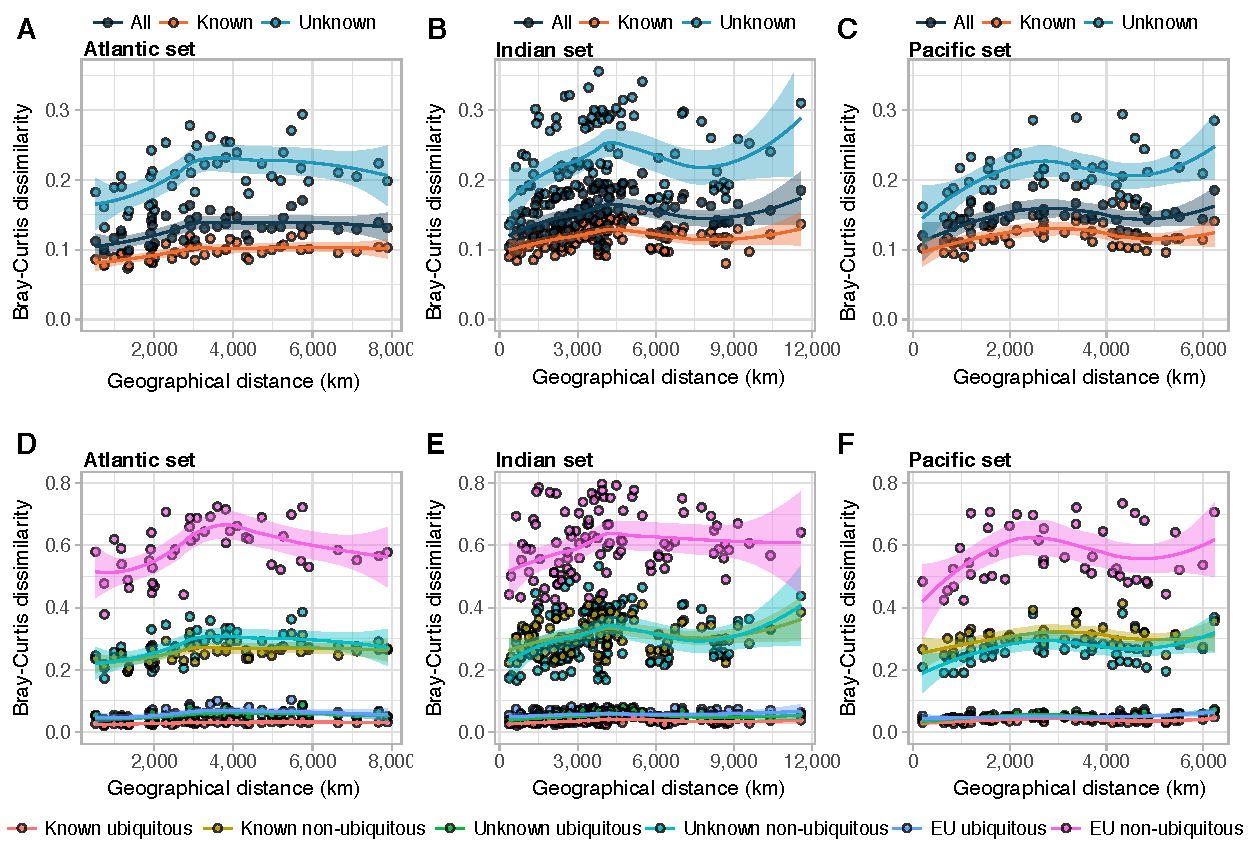
\includegraphics[width=1.0\textwidth] {fig_8}
	\caption[Sample sites beta-diversity vs. geographic distance - ubiquitous and non-ubiquitous components]{\textbf{Sample sites beta-diversity vs. geographic distance - ubiquitous and non-ubiquitous components.} (A-C). Distance-decay plot of TARA ocean surface, prokaryotic metagenomes by oceanic region defined in Figure~\ref{Fig:fig7} B. Sites appear six times defined by the EU (ubiquitous, non-ubiquitous), GU (ubiquitous, non-ubiquitous), and Knowns (ubiquitous, non-ubiquitous). The x-axis denotes the geographical distance between sampling sites, while the y-axis denotes the Bray-Curtis dissimilarity beta diversity measurement. (D-E) Box-plots of the Bray-Curtis dissimilarity beta diversity measurement for each component category.}\label{Fig:fig8}
\end{figure}

On the other hand, the larger Known matrix could have more noise due to its increased component list and be less sensitive to the Known adaptive protein signal, thus decreasing dissimilarity between sites.\\

When sites are defined by the Knowns they are the most similar in all ocean regions. This may be explained by the bias that Known components (Knowns with PFAM annotations) are protein sequences that are shared between a large fraction of the microbial community (e.g. housekeeping genes). This was indicated in the niche breadth analysis because around 25\% of the knowns had a wide niche breadth score.\\

The majority of our knowledge of Known microbial functions comes from essential/core gene experiments on cultured microbes that have been studied in the lab \citep{Bernard_2018}. Since our knowledge of protein functions are constrained by this, the Known fraction may be similar in all environments. Additionally, it has been shown that essential/core genes receive less purifying selection and are more conserved across the domains of life \citep{Jordan_2002}. Thus when sites are defined by Known components, dissimilarity is lower due to the overlap of known components between microbes.\\

\begin{table}[]
\centering
\caption{Mantel and Partial Mantel test to measure correlation (spearman) between beta-diversity and Haversine distance of TARA Ocean dataset.}
\label{table:3.4}
\begin{tabular}{@{}lcccc@{}}
\cmidrule[\heavyrulewidth](l){2-5}
                              & \multicolumn{2}{c}{Mantel test}  & \multicolumn{2}{c}{partial-Mantel test} \\ \cmidrule(l){2-5}
                              & {$\bm{\rho}$} & \textbf{p-value} & {$\bm{\rho}$}     & \textbf{p-value}    \\ \midrule
\textbf{Unknowns (EUs + GUs)} & 0.966         & 0.001            & 0.512             & 0.001               \\
\textbf{Knowns (K + Kwp)}     & 0.968         & 0.001            & 0.509             & 0.001               \\
\textbf{All combined}         & 0.965         & 0.001            & 0.515             & 0.001               \\ \bottomrule
\end{tabular}
\end{table}




%
%\begin{table}[]
%\centering
%\caption{Mantel and Partial Mantel test to measure correlation (spearman) between beta-diversity and Haversine distance of TARA Ocean dataset.}
%\resizebox{\textwidth}{!}{
%\begin{tabular}{llllll}
%\toprule
%\textbf{Component Category} & \textbf{Mantel statistic} & \textbf{p-value} & \textbf{partial-Mantel} & \textbf{p-value} \\
%\midrule
%\textbf{Unknowns (EUs + GUs)} & 0.966         & 0.001            & 0.512             & 0.001               \\
%\textbf{Knowns (K + Kwp)}     & 0.968         & 0.001            & 0.509             & 0.001               \\
%\textbf{All combined}         & 0.965         & 0.001            & 0.515             & 0.001               \\
%\bottomrule
%\end{tabular}}
%\label{Table:3.4}
%\end{table}
%

On a global scale, the Mantel test showed a significant positive correlation between genetic distance (Bray-Curtis) and geographical distance (Haversine) for the three component classes (Table~\ref{table:3.4}), indicating that closer samples are more similar than the distant. Those results are expected as the geographic isolation is related to the well-defined continental separation of the three oceanic regions used in the analyses: Atlantic, Pacific, and Indian. In all three ocean regions, when sampling sites are defined by All component categories, overall site dissimilarity increases in comparison to the Knowns. This is most likely because including the Unknown fraction in conjunction with the Known fraction increases overall site dissimilarity. The unique, site specific signal from the EUs and GUs may come from the rare biosphere and be environmentally adaptive proteins. This can add site unique component abundances which in turn increase dissimilarity between sites. Additionally, in all three ocean regions, each component category has a similar Bray-Curtis dissimilarity. This results hints that the relationship between the component categories may be a global ocean trend.\\

The All category represents the utilization of an entire metagenomic sample. In general, functional metagenomic analyses only compare ORFs that have known functions while the rest of the unannotated sequences are discarded. These analyses come in the form of heat maps \citep{McMahon_2015} or aggregated ordinations \citep{Louca_2016}. Here, it is demonstrated that incorporating the whole metagenomic sample into beta diversity measurements is informative and helps to highlight the dissimilarities between the samples.\\

Separate analyses were then performed on each individual region (Table~\ref{table:3.5}). This was done to remove the effect of continental masses distorting the distance decay-analysis, increase resolution of the analysis on the specific regions, and take advantage of the best transects the TARA Ocean sampling regime had to offer.\\

The Atlantic region had samples that transected the North Atlantic Ocean across the Gulf Stream (Figure~\ref{Fig:fig8} A, D). In Figure~\ref{Fig:fig8} A, there is a peak of dissimilarity in all three component categories at around 3,000 km. Increase in sample dissimilarity between 0 and 3,000 km is most likely due to the changing environment from coastal to open water. The dissimilarity then levels off from 3,000 km to 8,000 km. This could be due to the open water samples being in the Gulf stream. This ocean current pulls warm subtropical waters across the Atlantic towards Europe. The current may maintain similar environmental parameters as it crosses the Atlantic thus removing the distance-decay effect on microbial communities.\\

The Pacific and Indian sample regions had samples that followed a latitudinal North South transect (Figure~\ref{Fig:fig8} B, C, E, F). Both distance-decay plots follow a similar trend with an initial positive slope increase in dissimilarity, followed by a trough, then ending with dissimilarity increasing again. Previous findings have shown that environmental variation has more of an effect on functional group composition than dispersal limitation in the open ocean \citep{Louca_2016}. Additionally, temperature has been shown to be the main driving force for community composition in surface ocean waters \citep{Sunagawa_2015}. These observations are congruent with the curvature found in Pacific region distance-decay plot because similar environments can be found on either side of the equator in low or high latitudes. Latitudes equidistant from the equator receive similar solar radiation due to the curvature of the Earth and thus reflect similar temperatures (e.g. Arctic and Antarctic waters).\\

\begin{table}[]
\centering
\caption{Mantel and Partial Mantel test to measure correlation (spearman) between beta-diversity and Haversine distance in local in Atlantic, Pacific, and Indian ocean regions of TARA Oceans.}
\label{table:3.5}
\begin{tabular}{@{}lcccc@{}}
\cmidrule[\heavyrulewidth](l){2-5}
                              & \multicolumn{2}{c}{Mantel test}  & \multicolumn{2}{c}{partial-Mantel test} \\ \cmidrule(l){2-5}
                              & {$\bm{\rho}$} & \textbf{p-value} & {$\bm{\rho}$}     & \textbf{p-value}    \\ \midrule
\textbf{Unknowns (Atlantic)}  & 0.385 & 0.0201 & 0.0201 & 0.0240             \\
\textbf{Knowns (Atlantic)} & 0.475 & 0.0066 & 0.387 & 0.0240 \\
\textbf{All (Atlantic)} & 0.433 & 0.0120 & 0.417 & 0.0173 \\ \midrule
\textbf{Unknowns (Pacific)}  & 0.128 & 0.2528 & 0.086 & 0.3160 \\
\textbf{Knowns (Pacific)}  & 0.072 & 0.3384 & 0.046 & 0.3818 \\
\textbf{All (Pacific)}  & 0.111 & 0.2630 & 0.076 & 0.3317 \\ \midrule
\textbf{Unknowns (Indian)} & 0.068 & 0.3189 & 0.068 & 0.3070 \\
\textbf{Knowns (Indian)} & -0.196 & 0.8849 & -0.177 & 0.8595 \\
\textbf{All (Indian)} & -0.013 & 0.5159 & -0.013 & 0.5159 \\\bottomrule
\end{tabular}
\end{table}

%\begin{table}[]
%\centering
%\caption{Mantel and Partial Mantel test to measure correlation (spearman) between beta-diversity and Haversine distance in local in Atlantic, Pacific, and Indian ocean regions of TARA Oceans.}
%\resizebox{\textwidth}{!}{
%\begin{tabular}{llllll}
%\toprule
%\textbf{Component Category} & \textbf{Metagenomic set} & \textbf{Mantel statistic} & \textbf{p-value} & \textbf{partial-Mantel} & \textbf{p-value} \\
%\midrule
%\textbf{Unknowns (EU + GU)} & Atlantic & 0.385 & 0.0201 & 0.0201 & 0.0240 \\
%\textbf{Knowns (K + Kwp)} & Atlantic & 0.475 & 0.0066 & 0.387 & 0.0240 \\
%\textbf{All combined} & Atlantic & 0.433 & 0.0120 & 0.417 & 0.0173 \\
%\textbf{Unknowns (EU + GU)} & Pacific & 0.128 & 0.2528 & 0.086 & 0.3160 \\
%\textbf{Knowns (K + Kwp)} & Pacific & 0.072 & 0.3384 & 0.046 & 0.3818 \\
%\textbf{All combined} & Pacific & 0.111 & 0.2630 & 0.076 & 0.3317 \\
%\textbf{Unknowns (EU + GU)} & Indian & 0.068 & 0.3189 & 0.068 & 0.3070 \\
%\textbf{Knowns (K + Kwp)} & Indian & -0.196 & 0.8849 & -0.177 & 0.8595 \\
%\textbf{All combined} & Indian & -0.013 & 0.5159 & -0.013 & 0.5159 \\
%\bottomrule
%\end{tabular}}
%\label{my-label}
%\end{table}

\begin{figure}[h!]
	\centering
	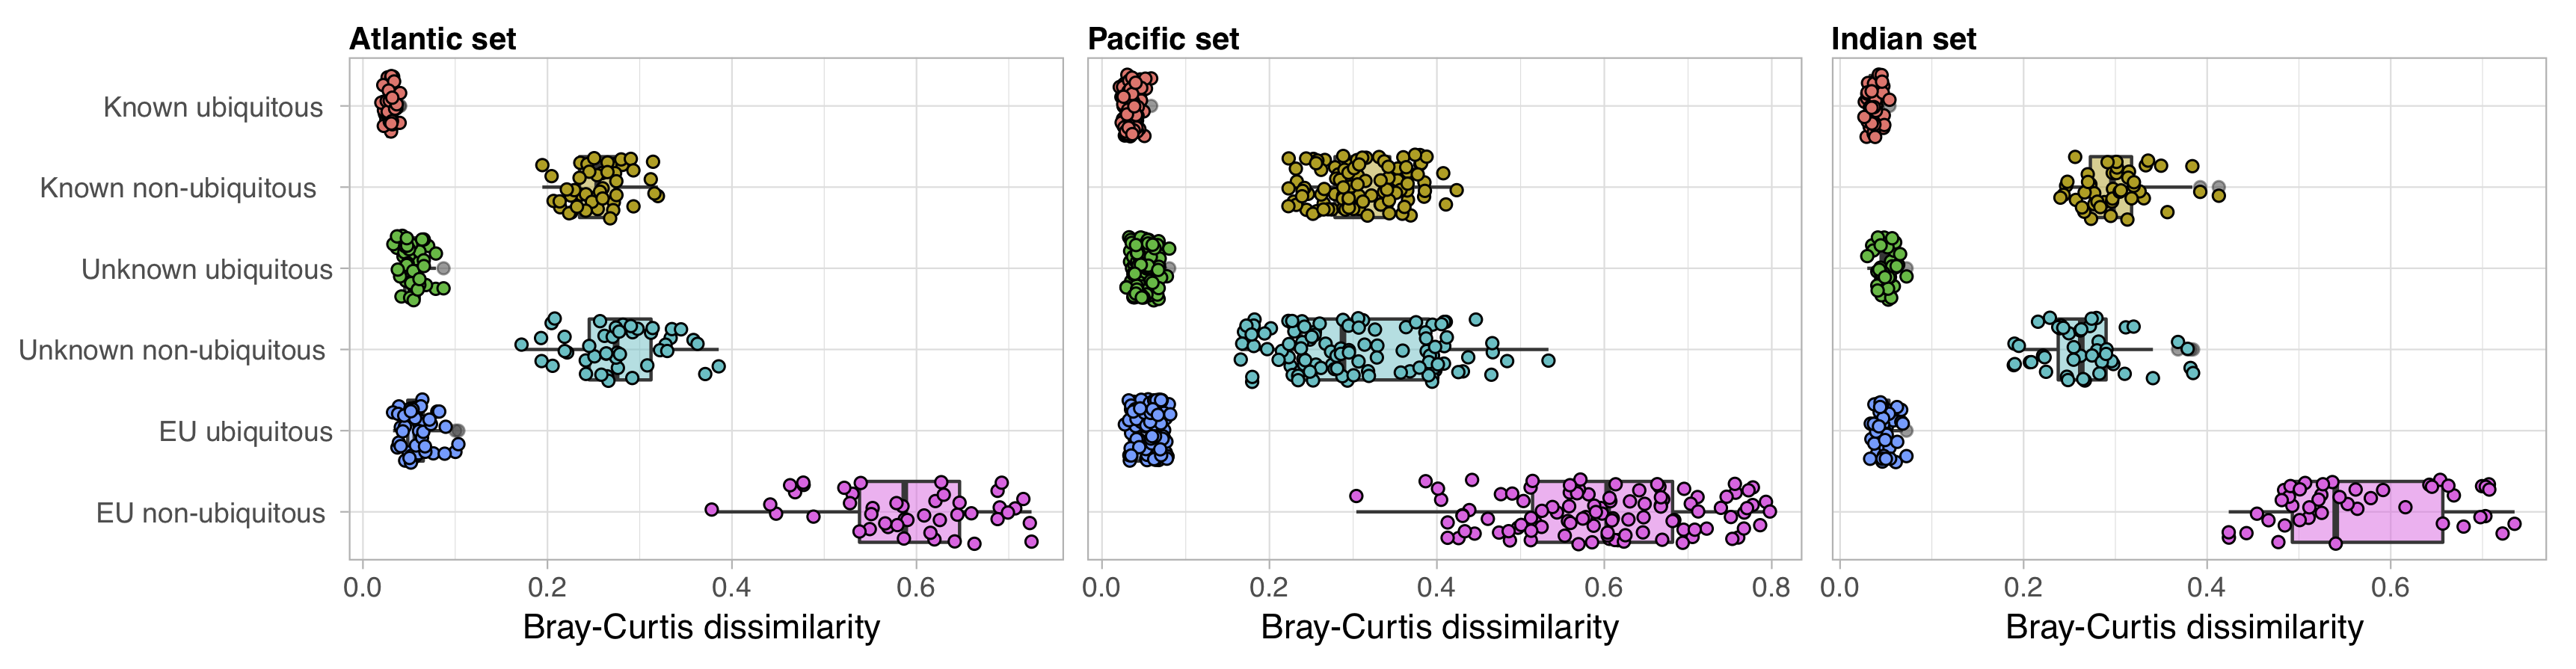
\includegraphics[width=1.0\textwidth] {fig_9}
	\caption[Beta-diveristy of ubiquitous vs non-ubiquitous components]{\textbf{Beta-diveristy of ubiquitous vs non-ubiquitous components.} Box plots representing the distribution of Bray-Curtis dissimilarity between sites in regions defined by \cite{Delmont_2017}.}
	\label{Fig:fig9}
\end{figure}

Another explanation for the distance-decay curvature that can be applied to both the Indian and Pacific regions is the sampling regimes moving away and back towards the coasts. Since the sampling paths start and return in similar environments across the gradient of open to coastal waters, component composition dissimilarity increases and decreases, responding to the environment. Though the Atlantic has a similar sampling structure, the Indian and Atlantic have a higher density of coastal samples. Both the Indian and Pacific distance-decay analysis have increases in dissimilarity at the farther geographic distances in the plot. This may be explained by the influence of the coastal environments selecting for unique component composition due to terrestrial runoff.

To further investigate if the Unknowns are site specific and adaptive proteins, component categories were separated and filtered into ubiquitous and non-ubiquitous fractions. The requirement for being ubiquitous was having a presence in every TARA ocean surface sample, anything less was considered non-ubiquitous. In all three ocean regions similar patterns emerge. When sites are defined by non-ubiquitous categories, EU defined sites are significantly more dissimilar than the other non-ubiquitous categories (Figure~\ref{Fig:fig8}). The Unknown and Known non-ubiquitous categories fall within a similar range of dissimilarity. On the other hand, the categories defined by ubiquitous fraction all fall into a very low, similar dissimilarity range of little no distance decay (Figure~\ref{Fig:fig8}).

The EU non-ubiquitous sites were overall the most dissimilar to each other. In light of the results from the ordination, and niche breadth analysis, this was an expected result. EUs have shown to be site specific, and are likely adaptive proteins. Removing the EU ubiquitous fraction that is found everywhere increases the site specific, adaptive signal even more, thus making sites more dissimilar. The non-ubiquitous EU fraction most likely drives the overall dissimilarity between sites when the entire metagenomic sample is taken into account.\\

The non-ubiquitous components all follow a similar distance-decay trend to their combined component analysis. This makes sense because non-ubiquitous components have a higher chance of being inherently adaptive because they are not found everywhere. In light of this, the non-ubiquitous fraction is most likely driving the distance-decay trends we observe.\\

When the ubiquitous fraction is removed from the Unknowns and Knowns their beta-diversity dissimilarities converge, and in the case of the Pacific and Indian region, overlap. This overlap in similarity is more than likely due to the similarity of the Kwp and GU component categories. GUs are taxonomically characterized in sequencing databases similar to Kwp but lack a functional annotation. On the scale of functional characterization, GUs and Kwp are the most similar by definition in the Vanni et. al. workflow. Due to their similarity within the design of the functional categories, they may have similar biogeographical patterns in the oceans. Another explanation is that the non-ubiquitous Knowns provide a more site specific, adaptive signal and drive dissimilarity to be more similar to the non-ubiquitous GUs. The niche breadth analysis showed that the Knowns have a similar distribution of narrow to wide B components. By removing the ubiquitous fraction, the narrow B components increase in relative abundance and thus drive the increase in dissimilarity.\\

The Unknowns may represent a hybrid of both \quotes{core} and environmentally adaptive proteins. The unknown ubiquitous fraction was making the unknown defined sites more dissimilar. There is a possibility that ubiquitous clusters could be involved in niche adaptation. It has been shown that core genes can be adaptive for the sugar metabolism in the metapangenome of \textit{Prochlorococcus} \citep{Delmont_2018}. Additionally, \cite{Delmont_2018} demonstrated that the accessory pangenome can be made up of environmental core and environmental accessory genes. This was determined by mapping metagenomic reads to the \textit{Prochlorococcus} and seeing in how many genomes the reads occurred. If an ORF is part of the core genome, then there may be a higher possibility that the protein is ubiquitous.\\

The ubiquitous fraction of every component category all followed a similar trend of defining sites as extremely similar with no significant distance decay. In other words, this group of components are found in every sample of the global regions analyzed and have a similar dissimilarity signal regardless of distance. These results were expected for the Knowns and possibly the GUs, but were surprising to see for the EUs. Due to the biases of protein characterization of essential genes in traditional microbial experiments, Known components contain a lot of housekeeping and essential functions (i.e. shared between all prokaryotes). Thus a strong and similar ubiquitous signal is to be expected. On the other hand, EUs have been shown to have a small niche breadth and be adaptive responses to the environment (as seen in the niche breadth analysis). The signal of ubiquitous EU components, which have no functional annotation or are found in sequenced or draft genomes, is not in line with the previous results in this thesis. This may demonstrate that the EUs share core microbial functions with the other component categories in the world's oceans. This is a surprising results because it could infer that a set of proteins from a ubiquitous domain of life and or function in the ocean have been left uncharacterized by metagenomics. In total, 6,587 EUs are in this category and were subjected to further investigation. \\

\section{Investigating the Ubiquitous EU fraction}

To demonstrate that the ubiquitous EU fraction is a legitimate functional signal, we took steps to remove spurious proteins and to detect distant homology and taxonomy (Table~\ref{table:3.6}). First we ran antiFAM HMMERs against the potential EU sequences. This removed 250 spurious proteins from the component set. Next, HHblits detected distant homology in 4,823 of the potential EUs with 3,811 having their best hit being a Hypothetical or uncharacterized protein. Finally, for the EUs that were not hit by HHblits we assigned taxonomy using Kaiju, 81 EUs were classified (Table~\ref{table:3.7}). This left us with 1,514 potential EUs with no distant homology or taxonomy.\\

HHblits iteratively compares one HMM against another HMM to detect distant homologies. HMM vs HMM is the most effective technique for detecting distant homologs because it can detect the similarity of the structural templates that usually diverge slower than the sequences themselves. Proteins may remain structurally very similar long after their sequence similarity has been lost. The fact that HHblits was able to detect distant homology in 4,823 EUs indicates that some of the Vanni et. al. EU components may in fact be GUs. This caveat has been solved in the upcoming version of the workflow (Vanni et. al. in prep). HHblits did however fail to detect distant homology in the 1,514 ubiquitous EUs. This was either because they are truly novel, or simply an artifact of sequencing or assembly.\\

We used Kaiju with the objective to gather taxonomic information of the ubiquitous EUs using a k-mer based approach that in theory is less database biased. The tool takes advantage of the fact that different taxa have different amino acid compositions signatures.\\

\begin{table}[H]
\centering
\caption{Exploration of ubiquitous EUs (6,587) taxonomy and homology to databases}
\label{table:3.6}
\begin{tabular}{ll}
\toprule
\textbf{Ubiquitous EU classification step} & \textbf{Number of ubiquitous EUs} \\
\midrule
\textbf{Removed with antiFAM} & 250 \\
\textbf{HHblits distant homology detected} & 4,823 \\
\textbf{Kaiju taxonomy classified} & 81 \\ \midrule
\textbf{Potential EU} & \textbf{1,514} \\
\bottomrule
\end{tabular}
\end{table}

This strategy is unique compared to other more traditional nucleotide methods like Kraken \citep{Wood_2014}. Thus, the Kaiju hits only imply there is a similar k-mer frequency between the 81 Kaiju hits and any of the taxa on NCBI nr database. \\

\begin{table}[H]
\centering
\caption{Kaiju taxonomic annotation of ubiquitous potential EUs with no distant homology}
\label{table:3.7}
\begin{tabular}{ll}
\toprule
\textbf{Kaiju taxonomic assignment} & \textbf{Number of ubiquitous EUs} \\
\midrule
\textbf{Bacteria} & 64 \\
\textbf{Eukaryota} & 3 \\
\textbf{Environmental} & 14 \\ \midrule
\textbf{Total} & \textbf{81} \\
\bottomrule
\end{tabular}
\end{table}

Kaiju did not detect taxonomy in all of the ubiquitous EUs. This may have occurred for a few reasons. First, some ubiquitous EUs may be a new expansion of the tree of life, similar to the Candidate Phyla Radiation \citep{Danczak_2017}, and thus have a unique k-mer frequency. Second, they are sequencing artifacts and errors, thus have a random, non-related k-mer frequency to known taxa. A future direction for the Vanni et. al. workflow could be to add tool Spurio to the cluster validation steps to identify and remove spurious genes \citep{H_ps_2018}. \\

In light of ubiquitous vs non-ubiquitous genes, the discussion of \quotes{core} or \quotes{essential} microbial functions can be brought up. The current understanding of \quotes{core} genomic functions and metabolic pathways is heavily biased by the low number of deeply characterized microbes grown in the lab \citep{Prosser_2014}. The core functions found in common in laboratory isolate may not be representative of the total environmental \quotes{core}. The Ubiquitous EUs may be a new \quotes{core} set of genes that have only been detected by means of environmental gene content comparison. \\

\section{Mapping EUs to TARA Ocean MAGs}

The onset of techniques to extract metagenomic assembled genomes (MAGs) from metagenomic samples has allowed for great insight into microbial populations. Deeper sequencing technology, allowing for 50x of less abundant microbial populations, and efficient differential coverage binning algorithms has led to an era of Metagenomics 2.0 \citep{McMahon_2015}. Additionally, MAGs can now be manually curated in an efficient manner leading to higher quality \citep{Eren_2015}. Although MAGs represent populations of similar microbes and are not complete genomes, the binned contigs are a step closer to the genetic units they came from, genomes. EUs that successfully mapped to the \cite{Delmont_2017}  MAGs were then upgraded to a new category of the unknown, Population Unknowns.\\

\textbf{Population Unknowns (PU)}\\
ORF clusters with an unknown function but map to contigs in MAGs.

To investigate further if the ubiquitous EU components are indeed real proteins found in the environment, we mapped the clusters belonging to the selected components against a set of high quality metagenomic assembled genomes binned from the TARA Ocean prokaryotic dataset \citep{Delmont_2017}. Finding ubiquitous EUs in MAGs from the environment they originated from increases the chance of the component being indeed a real environmental protein sequence because it is occurring in the context of a population of similar genomes in the environment. \\

\begin{figure}[h!]
	\centering
	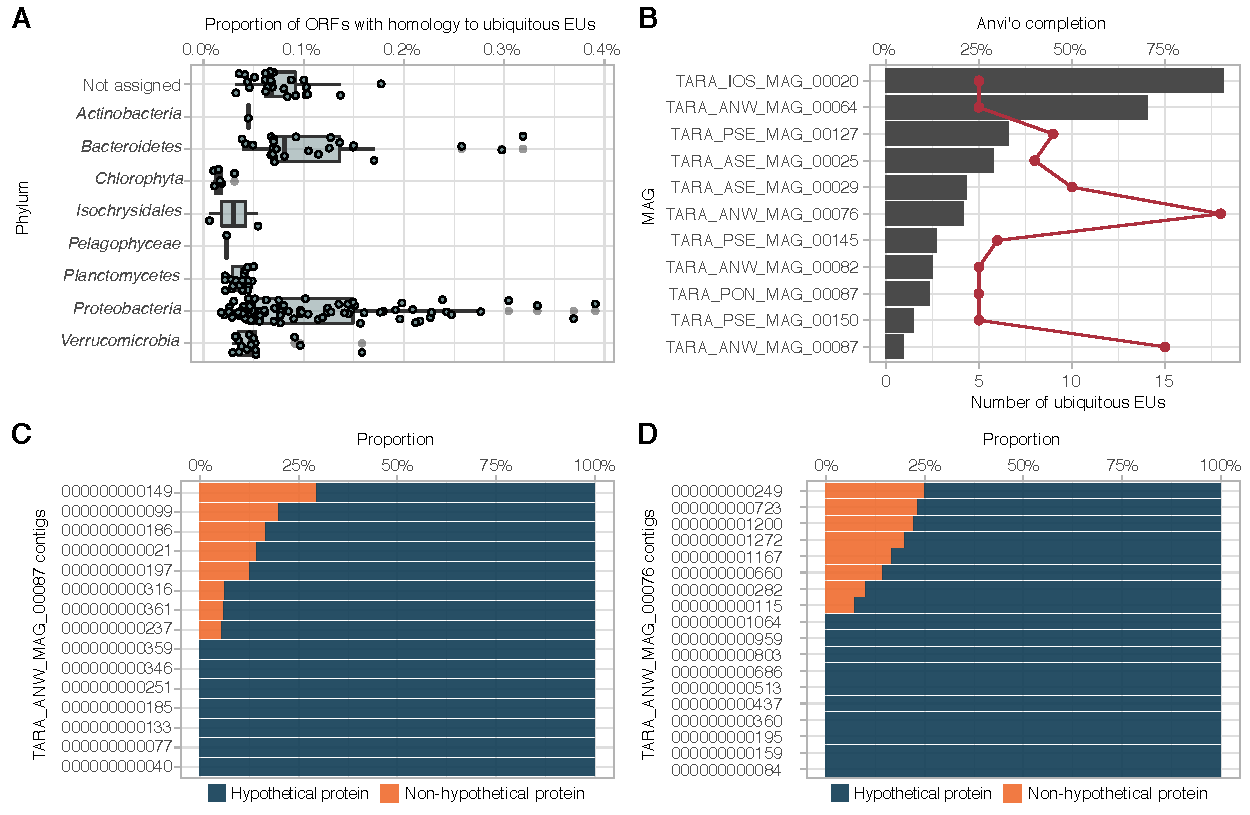
\includegraphics[width=1.0\textwidth]{fig_10}
	\caption[EU mapping results]{\textbf{EU mapping results} A) Proportions of ORFS with homology to potential EU within TARA MAGs. X axis is the op hit phylum of potential EU mapping to TARA MAGs. B) Histogram of TARA MAG percent completeness (checkM). Red line represents the number of Potential EUs found in the MAGs. C-D) Contigs from TARA MAGs TARA\_ANW\_MAG\_00076 and TARA\_ANW\_MAG\_00087 in descending order of highest proportion of non-hypothetical ORF content.}
	\label{Fig:3.9}
\end{figure}

Out of the 957 non-redundant MAGs, the ubiquitous EUs mapped to 178 of them. This is a significant amount of the MAGs. If the potential origin of the ubiquitous EUs is from organisms that are part of the rare biosphere, this means that the TARA Ocean project sampled at a critical moment when the rare microbes \quotes{bloomed} due to conducive environmental conditions \citep{Gobet_2011}. In order to be binned into MAGs, there has to be enough sequencing depth and coverage of the population. Continual deep sequencing of marine waters is needed to catch more of the rare biosphere for metagenomic assembly and expand our knowledge of the world oceans.
Our next goal was to examine the genomic neighborhood of the ubiquitous EUs on the contig of which they mapped to. Investigating the genomic neighborhood can lead to the inference of a possible function of the EU. Furthermore, if the EU is surrounded by genes of known function, this adds clarity that the EU is a part of a real contig and possibly an operon.\\

To select which MAG contig to visualize, we picked the MAGs with the least completeness and highest number of ubiquitous EUs mapped to it (Figure~\ref{Fig:3.9} B). Next we selected contigs to visualize by choosing the ones with the highest proportion of non-hypothetical proteins (Figure~\ref{Fig:3.9} C-D). The more annotated proteins on the contig, the more genomic context we can apply to the ubiquitous EU. \\

TARA ocean MAGS TARA\_ANW\_MAG\_00076 and TARA\_ANW\_MAG\_00087 were selected for contig analysis because they were the most enriched with ubiquitous EUs (Figure~\ref{Fig:3.9} B). These mags originated from the South West Atlantic Ocean TARA sampling sites. We then picked contigs where the ubiquitous EUs mapped to and arranged them based on content of non-hypothetical genes (Figure~\ref{Fig:3.9} C-D). This was in order to have a higher chance of having the ubiquitous EU surrounded by genes of known function. If the ubiquitous EU is surrounded by genes of known function, it adds another layer of evidence that the EU is indeed a real sequence. If the EU was spurious, multiple levels of the metagenomic analysis to make the MAG would have had gone wrong including gene prediction, assembly and binning.  \\

\begin{figure}[h!]
	\centering
	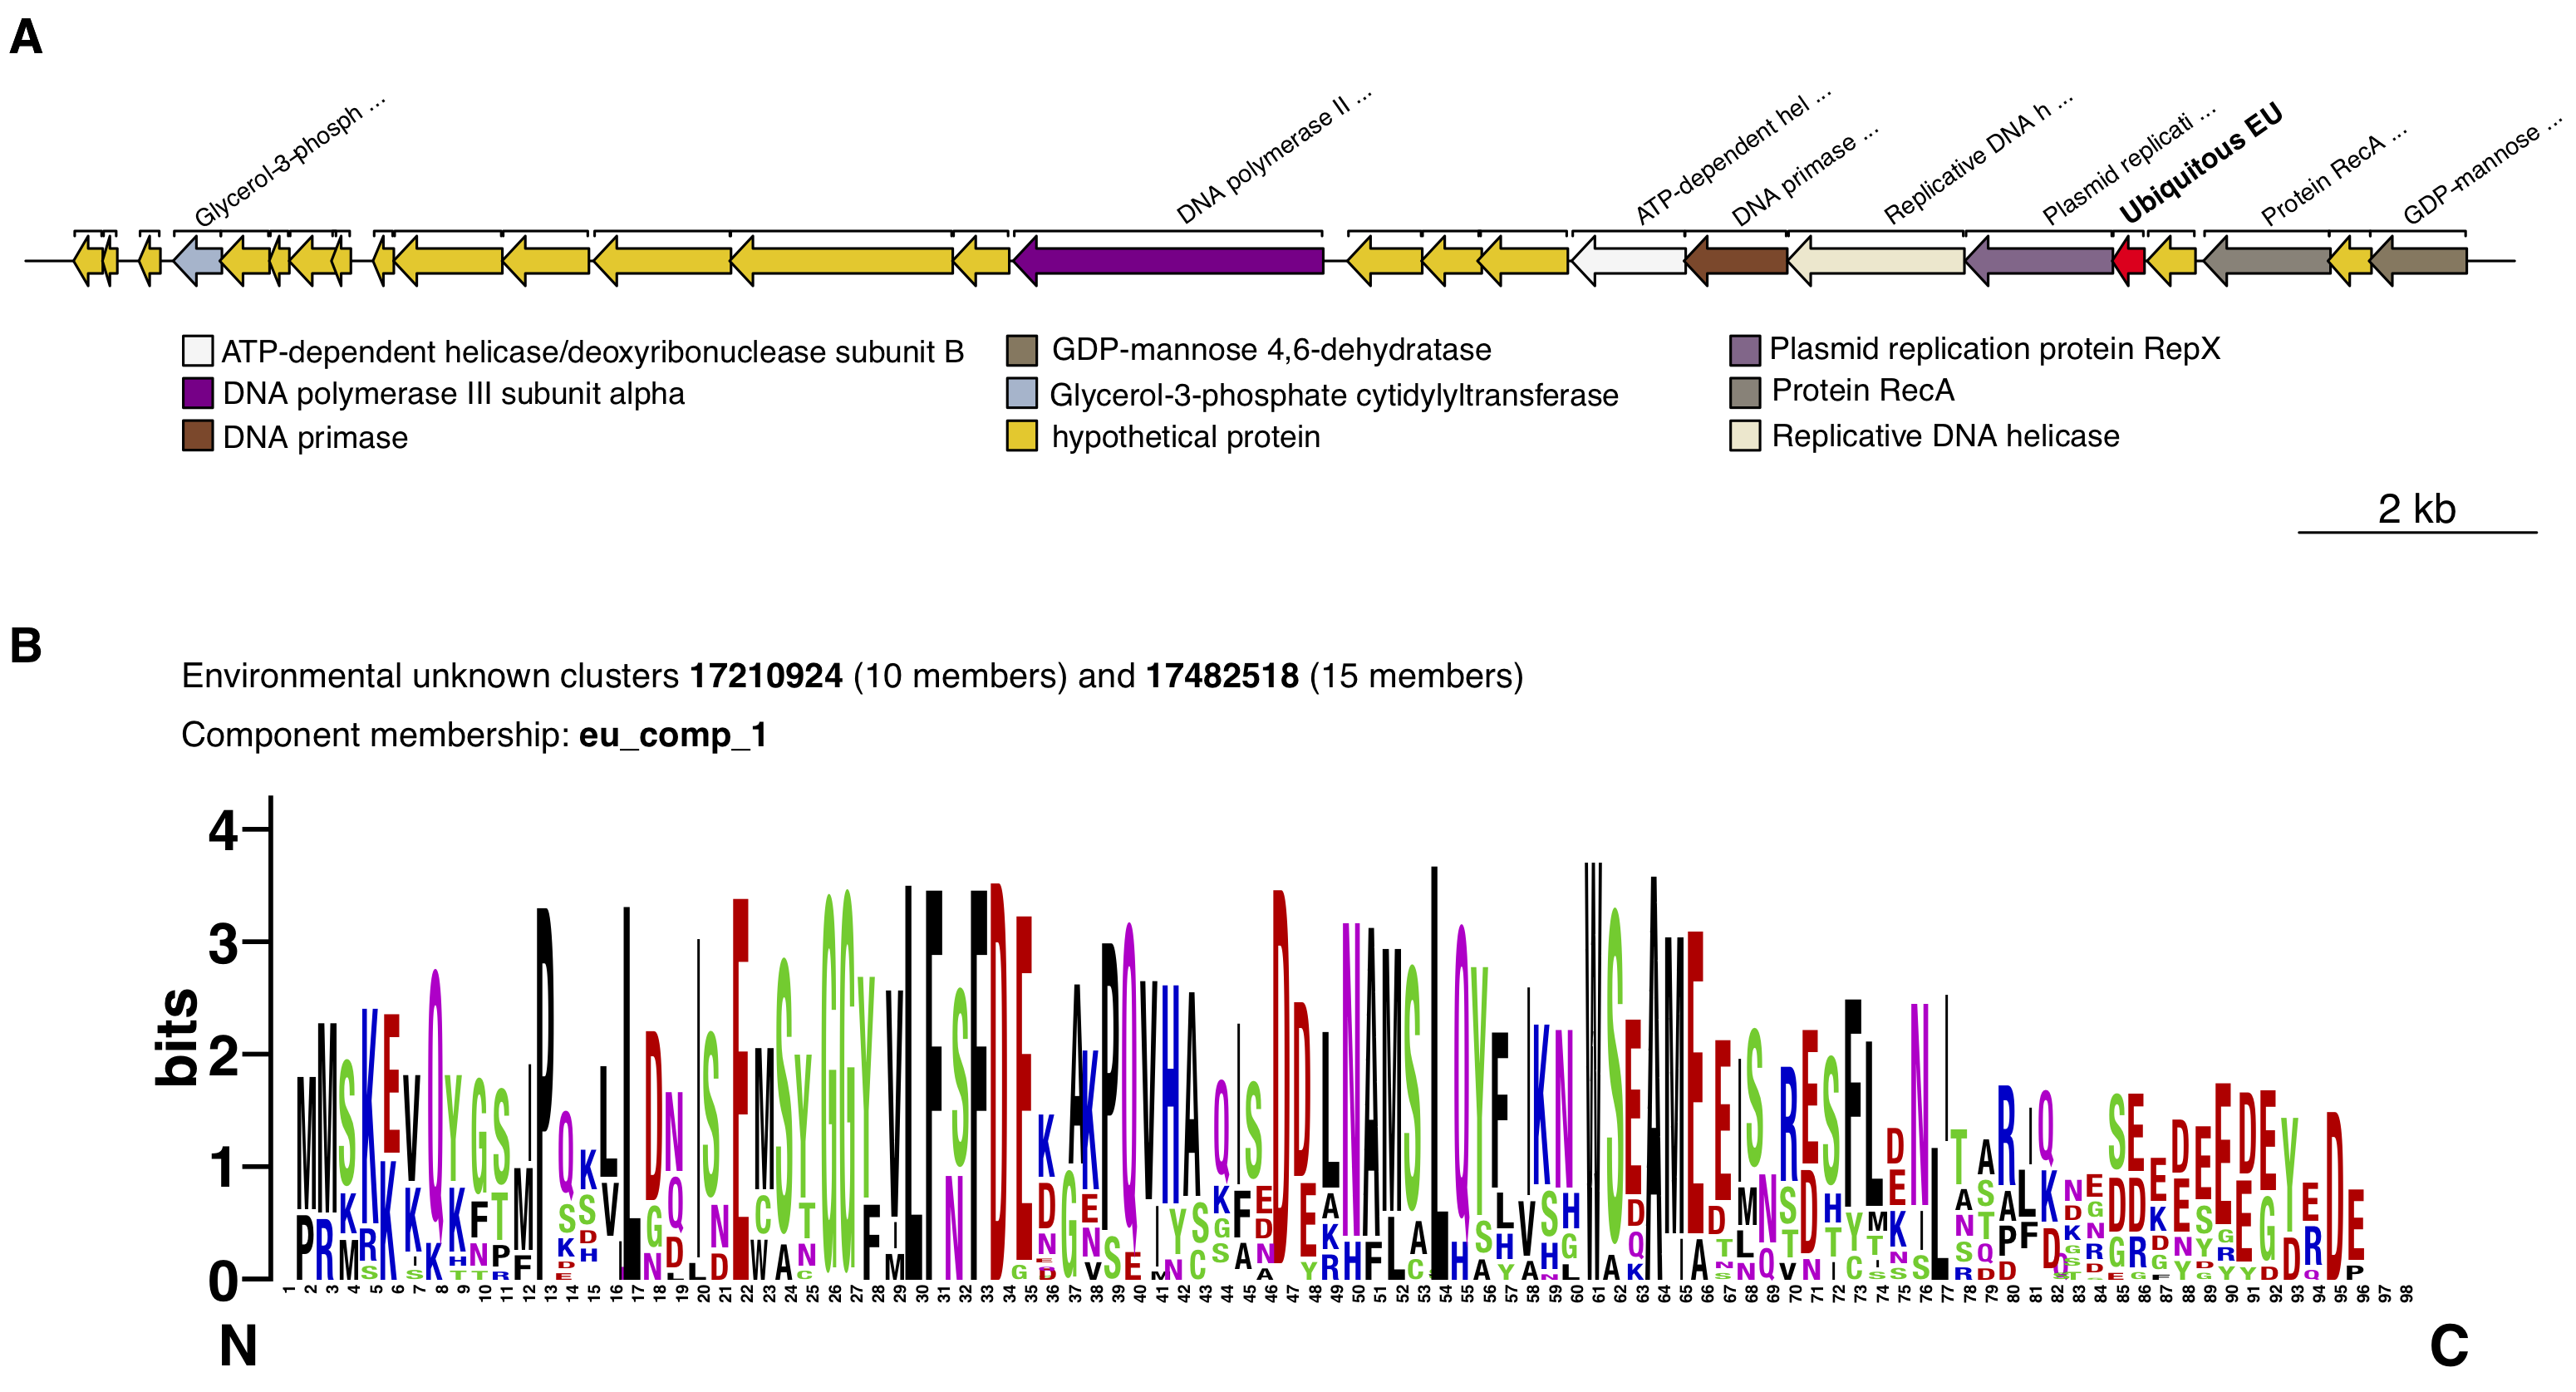
\includegraphics[width=1.0\textwidth] {fig_11}
	\caption[EU gene visualization]{\textbf{EU gene visualization.} A) Contig genomic neighborhood around a potential EU. B) Conserved consensus sequence logo of of eu\_com\_1.}
	\label{Fig:3.10}
\end{figure}

In Figure~\ref{Fig:3.10} A, contig TARA\_ANW\_MAG\_00087\_000000000149 is shown. Highlighted in red, is the predicted ORF with significant homology Environmental Unknown clusters (17210924 and 17482518) members of the ubiquitous EU component eu\_comp\_1 (The EU was blasted against NCBI nt and NCBI genomes to see if there was any significant match to nucleotide sequences in databases). Within its genomic neighborhood are genes relating to DNA and plasmid replication and repair including DNA polymerase II, DNA primase, and protein RecA. Gene placement in prokaryotic genomes is not random. Genes are grouped together to increase transcriptional efficiency to respond to stimuli in the environment. The lac operon is an example of a group of genes that are transcribed together to metabolize lactose. Since this ubiquitous EU is associated with these DNA and plasmid repair genes, we can hypothesize that it has a related function. Another aspect to consider is that the surrounding genes are essential/core functions for microbial life. Without DNA repair mechanisms, genetic integrity of species would not be able to be maintained. Considering that the ubiquitous EU is surrounded by essential \quotes{ubiquitous} biological functions and is found in every sample in the TARA Ocean dataset, there is a higher chance this is a real protein. Furthermore, the consensus amino acid residues after aligning all sequences from both clusters belonging to the component eu\_comp\_1 (Figure~\ref{Fig:3.10}B) contain two active residues (E, D), one of the conditions defined to identify non-spurious ORFs by \cite{Li_2008}, supporting one more time that the ORF might be real. \\

The ubiquitous EUs that were not found in the MAG data set or detected for distant homology have the potential of being part of the genomic repertoire of members present in the rare biosphere. There is mounting evidence that the theory in microbial ecology that \quotes{everything is everywhere} but is selected for by the environment is indeed true \citep{Gibbons_2013}. All ocean samples may contain a \quotes{microbial seed bank} where many rare taxa exist in stationary phase or grow extremely slowly \citep{ Pedros_2006}. This theory has mainly been investigated via 16S rDNA amplicon sequencing because the scientific question was focused on phylogenetic diversity. With deeper sequencing, immense diversity of low abundance microbes have been recovered. New protein families have been detected before via mass sequencing efforts and protein clustering \citep{Yooseph_2007}. The difference made in this analysis was the Unknown fraction was put in a functional biogeographical context. Due to the deep metagenomic sequencing of the TARA ocean dataset, this maybe the first time that \quotes{core} functions from the rare biosphere have been revealed. Due to the Vanni et. al. Unknown cluster categories, the unannotated protein diversity of the TARA ocean data set was able to be accounted for.\\
% Conclusion and Outlook

% Chapter Template

\chapter{Conclusion and Outlook} % Main chapter title

\label{Conclusion and Outlook} % Change X to a consecutive number; for referencing this chapter elsewhere, use \ref{ChapterX}

%\lhead{Chapter 1. \emph{Introduction}} % Change X to a consecutive number; this is for the header on each page - perhaps a shortened title

\renewcommand{\chaptermark}[1]{\markboth{#1}{}}
\renewcommand{\sectionmark}[1]{\markright{#1}}
\fancyhead[RE]{\small\leftmark}
% Section in the left on even pages}
\fancyhead[LO]{\small\rightmark}%Section in the left on odd pages

%\section{A section goes here}

In this thesis, we have shown that including the entire metagenomic sample in functional biogeography is key to resolve difference between sampling sites. Regardless if a protein cluster has an annotation, it can be accounted for in samples and help define minute differences between geographical sites. By defining a site by their complete functional repertoire, unique insights were generated about the TARA Ocean Southern Ocean sampling sites not observed in the original TARA analysis \citep{Sunagawa_2015}. The Vanni et. al. 2018 clusters lay the groundwork for accounting for the entire metagenomic sample and has many future applications in functional microbiology research.\\

\textbf{Unknowns as indicators}\\


One direction for immediate application could be to include the Unknowns in objectives for genomic observatories. Since EUs and GUs were associated with small niche occupancy and are selected due to specific environmental factors, their abundances may be good indicators for environmental pollution. Microbial populations respond fast to environmental changes and thus are good indicators for ecosystem health and stress \citep{Buttigieg_2018}. Genomic observatories monitor this phenomena to determine ecosystem health \citep{ Davies_2012}. With the immense influx of high-throughput next-generation sequencing (NGS) data, genomic observatories can effectively monitor ecosystem changes using predictive strategies. \cite{ Buttigieg_2018} makes the case that a deeper understanding of ocean microbial interactions and functions will improve biomonitoring. It was recently shown that machine learning approaches can effectively analyze differences in ocean microbial taxa can effectively predict anthropogenic impacts \citep{Cordier_2017}. A future direction for the Unknowns could be to train Random Forest (RF) algorithms to predict the anthropogenic impacts on the environment and find reliable indicators for environmental monitoring.
Including all predicted ORFs in a sample not only adds information to the site, but also is a better return on investment of the sequencing effort itself. Millions taxpayer dollars and euros have been spent on large environmental sequencing efforts. It is a waste of resources that in most cases not all information for the DNA samples is gleaned and the unannotated fraction is discarded.\\

A general theme in this thesis was the application of traditional ecological methods to analyze the distribution of the Unknown fraction. Through Levin\textquotesingle s Niche Breadth and biogeographical analysis we were able to show unique insights about unknown ubiquitous functions in the ocean. Multidisciplinary approaches may be the key to uncovering more insights about functional biogeography in the world's oceans. There is already dialogue discussing how to apply traditional population genetics methods to the core and accessory genes of the pangenome. Another future direction for the research into the Unknown fraction is to examine their distribution in pangenomes. Research questions can be addressed such as are the Unknowns enriched in the core genome, are Unknowns associated with different phylotypes?  \\

\textbf{Revealing the function of unknowns}\\

If 99\% of microbes are currently uncultivable in the laboratory \citep{Barer_2015}, it can be assumed that many functions will remain unknown until more are isolated and cultured. Computational approaches to marine microbiology have their limitations. Regardless if sequencing technology continues to increase in sequencing depth and quality, gene prediction, assembly, and binning algorithms will never be perfect. NGS data will always be subjected to sequencing and post-processing artifacts. Bioinformatics provides a great platform for hypothesis generation to select and search for important Unknowns, but to truly characterize the Unknown, laboratory experiments on cultured isolates are an absolute necessity. If the Ubiquitous EU component signal is indeed coming from the rare biosphere many innovations will be needed to create cutting edge culturing methods to grow these bugs in the laboratory. The potential of new microbial functions in the rare biosphere is immense and worth investigating due to the untapped resources for biotechnology, environmental applications, and fundamental knowledge. \\

Another step to investigate the ubiquitous EU would be to express them in microbial vectors and test their function. Many methods are developing to efficiently screen metagenomic libraries, select contigs, and express them in vectors \citep{Leis_2013}. Once expressed, novel genes can be quickly tested for their functions in assays.\\

Similar to how \cite{Wyman_2017}  created a list of most wanted FUnkFams, this ecological analysis of the Unknown component fraction is a starting point for targeted environmental protein analysis. Analyzing the patterns and distribution of the Unknown from an ecological perspective can lead to more insights about microbial functions. Additionally, the more functions that are uncovered, the more predictive power genomic observatories may have to detect minute changes in the environment.\\

It has been suggested that genes of hypothetical function that are conserved throughout phyla should be prioritized for characterization\citep{Galperin_2004, Hanson_2010}. The \quotes{core} set of genes have the potential to uncover new phylogenetic markers and essential functions for the definition of life on this planet. This philosophy should be extended to environmentally conserved protein clusters, in particular the Environmental Unknown Ubiquitous clusters.\\
%\input{Chapters/Chapter7}

%%% acknoledgegements

%\input{{\acknowledgements{\addtocontents}} % Add a gap in the Contents, for aesthetics

%The acknowledgements and the people to thank go here, don't forget to include your project advisor\ldots
%}
%\addtocontents{toc}{\vspace{2em}} % Add a gap in the Contents, for aesthetics
%\acknowledgements % Cue to tell LaTeX that the following 'chapters' are Appendices
\let\cleardoublepage\clearpage
\addtocontents{toc}{\vspace{2em}} % Add a gap in the Contents, for aesthetics
\appendix % Cue to tell LaTeX that the following 'chapters' are Appendices
\begin{appendices}
\renewcommand\chaptername{Appendix}
\renewcommand{\chaptermark}[1]{\markboth{#1}{}}
\renewcommand{\sectionmark}[1]{\markright{#1}}
\fancyhead[RE]{\small\leftmark}
% Section in the left on even pages}
\fancyhead[LO]{\small\rightmark}%Section in the left on odd pages

\chapter[Appendix]{}% Main chapter title
%\chaptermark{}

%\label{Appendix1} % Change X to a consecutive number; for referencing this chapter elsewhere, use \ref{ChapterX}


%\blindtext[10]

\begin{figure}[h!]
	\centering
	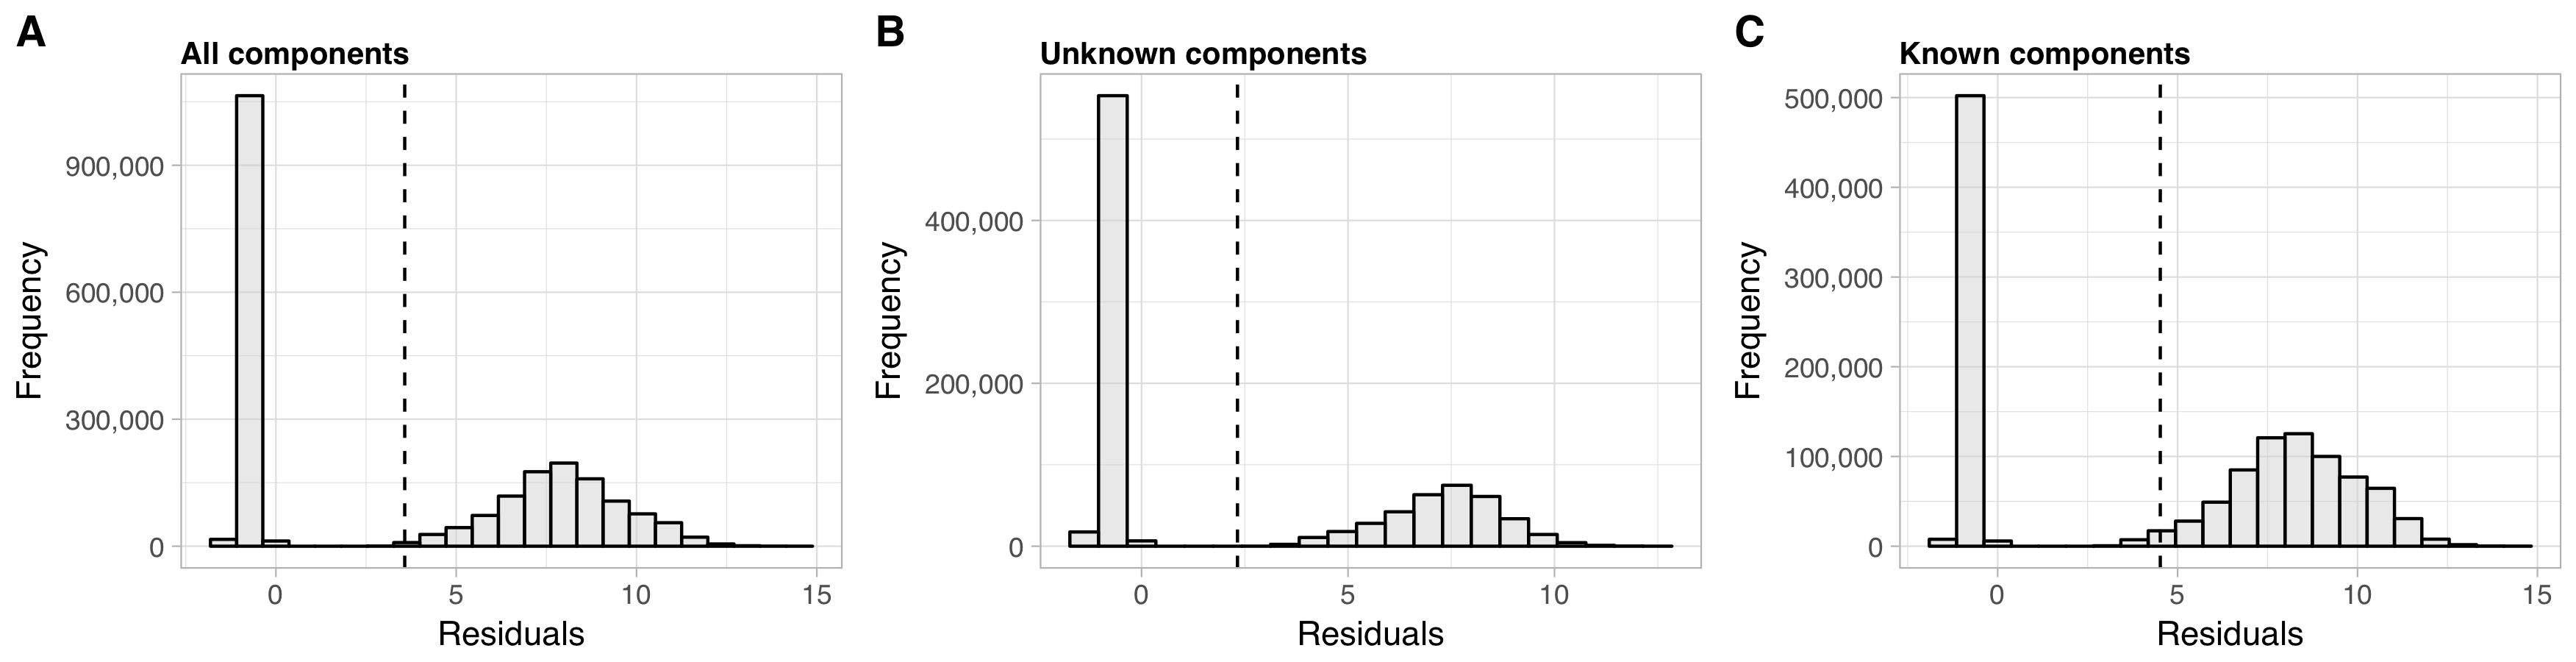
\includegraphics[width=1.0\textwidth] {fig_s1}
	\caption[TARA Oceans PCA residuals histogram]{\textbf{TARA Oceans PCA residuals histogram.} A) Residuals of PCA with sites defined by all components. B) Residuals of PCA with sites defined by at the unknown components (EUs + GUs). C) Residuals of PCA with sites defined by the Known components (K + Kwp).}
	\label{Fig:A1}
\end{figure}

\begin{figure}[h!]
	\centering
	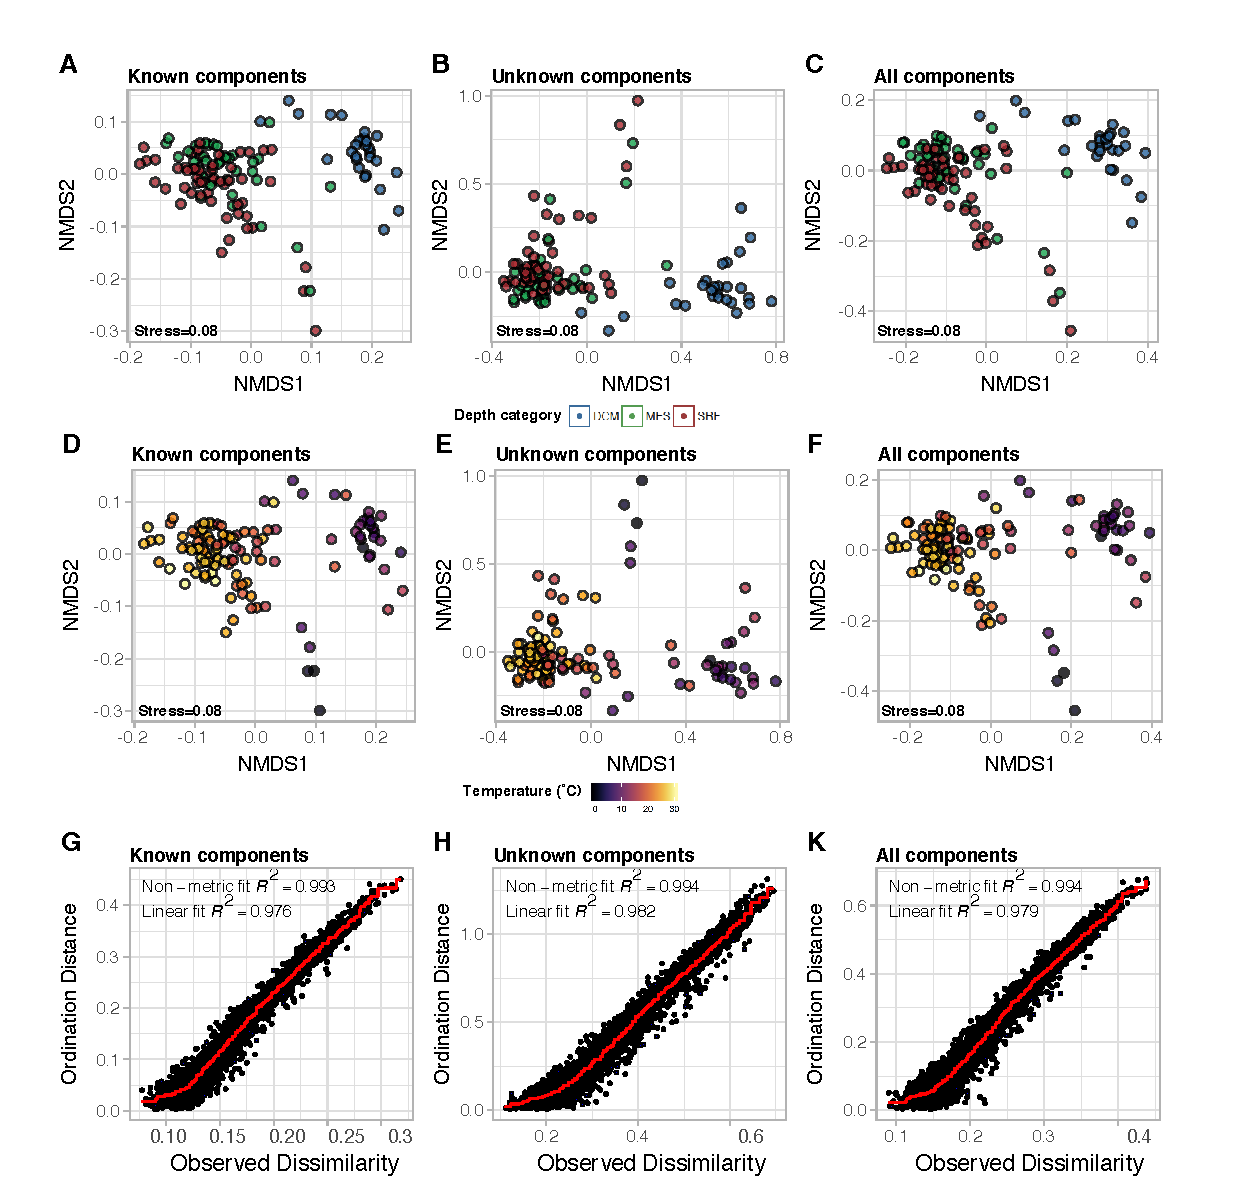
\includegraphics[width=1.0\textwidth] {nmds_panel.pdf}
	\caption[TARA Oceans NMDS and Shepard Plots]{\textbf{TARA Oceans NMDS and Shepard Plots.} A-C) TARA ocean metagenomes defined by (A) Knowns (K + Kwp), (B) Unknowns  (EUs + GUs), and (C) ALL components. Sites are colored by depth of origin (Red = surface, Green = deep chlorophyll maximum, and Blue = mesopelagic. D-E) Same plots as A-C but colored by temperature. The darker the color, the colder the sea water temperature. G-I) Shepard plots for NMDS in A-F }
	\label{Fig:A2}
\end{figure}

\end{appendices}

% Include the appendices of the thesis as separate files from the Appendices folder
% Uncomment the lines as you write the Appendices
%\chapter*{Bibliography}
\addcontentsline{toc}{chapter}{Bibliography}

%\chapter{Discussion and Perspectives} % Main chapter title

%\label{Chapter6} % Change X to a consecutive number; for referencing this chapter elsewhere, use \ref{ChapterX}

%\lhead{Chapter 6. \emph{Discussion and Conclusions}} % Change X to a consecutive number; this is for the header on each page - perhaps a shortened title


Adam P, Schneckenburger P, Schaeffer P, Albrecht P. (2000). Clues to early diagenetic sulfurization processes from mild chemical cleavage of labile sulfur-rich geomacromolecules. Geochim Cosmochim Acta 64:3485-3503.

Aller RC. (1994). Bioturbation and remineralization of sedimentary organic matter: effects of redox oscillation. Chem Geol 114:331-345.

Archer D, Maier-Reimer E. (1994). Effect of deep-sea sedimentary calcite preservation on atmospheric CO$_2$ concentration. Nature 367:260-263.

Armstrong RA, Lee C, Hedges JI, Honjo S, Wakeham SG. (2001). A new, mechanistic model for organic carbon fluxes in the ocean based on the quantitative association of POC with ballast minerals. Deep Sea Res Part II Top Stud Oceanogr 49:219-236.

Arndt S, J{\o}rgensen BB, LaRowe DE, Middelburg JJ, Pancost RD, Regnier P. (2013). Quantifying the degradation of organic matter in marine sediments: A review and synthesis. Earth-Science Rev 123:53-86.

Arnosti C. (2011). Microbial Extracellular Enzymes and the Marine Carbon Cycle. Ann Rev Mar Sci 3:401-425.

Arnosti C, Bell C, Moorhead DL, Sinsabaugh RL, Steen a. D, Stromberger M, et al. (2013). Extracellular enzymes in terrestrial, freshwater, and marine environments: perspectives on system variability and common research needs. Biogeochemistry 117:5-21.

Arrieta JM, Mayol E, Hansman RL, Herndl GJ, Dittmar T, Duarte CM. (2015). Dilution limits dissolved organic carbon utilization in the deep ocean. Science (80) 348:331-333.

Arthur MA, Dean WE, Pratt LM. (1988). Geochemical and climatic effects of increased marine organic carbon burial at the Cenomanian/Turonian boundary. Nature 335:714-717.

Badertscher S, Fleitmann D, Cheng H, Edwards RL, G\"okt\"urk OM, Zumb\"uhl a., et al. (2011). Pleistocene water intrusions from the Mediterranean and Caspian seas into the Black Sea. Nat Geosci 4:236-239.

Baird D, Christian RR, Peterson CH, Johnson GA. (2004). Consequences of hypoxia on estuarine ecosystem function: energy diversion from consumers to microbes. Ecol Appl 14:805-822.

Baird D, Ulanowicz RE. (1989). The seasonal dynamics of the Chesapeake Bay ecosystem. Ecol Monogr 59.

Ball DF. (1964). Loss-on-ignition as an estimate of organic matter and organic carbon in non-calcareous soils. J Soil Sci 15:84-92.

Baturin GN. (2007). Issue of the relationship between primary productivity of organic carbon in ocean and phosphate accumulation (Holocene-Late Jurassic). Lithol Miner Resour 42:318-348.

Belmar L, Molina V, Ulloa O. (2011). Abundance and phylogenetic identity of archaeoplankton in the permanent oxygen minimum zone of the eastern tropical South Pacific. FEMS Microbiol Ecol 78:314-26.

Bentley DR, Balasubramanian S, Swerdlow HP, Smith GP, Milton J, Brown CG, et al. (2008). Accurate whole human genome sequencing using reversible terminator chemistry. Nature 456:53-9.

Berelson WM, Hammond DE, McManus J, Kilgore TE. (1994). Dissolution kinetics of calcium carbonate in equatorial Pacific sediments. Global Biogeochem Cycles 8:219-235.

Bernardet J, Nakagawa Y, Holmes B. (2002). Proposed minimal standards for describing new taxa of the family Flavobacteriaceae and emended description of the family. Int J Syst Evol Microbiol 52:1049-1070.

Berner RA. (1990). Atmospheric carbon dioxide levels over phanerozoic time. Science 249:1382-6.

Berner RA. (1989). Biogeochemical cycles of carbon and sulfur and their effect on atmospheric oxygen over phanerozoic time. Palaeogeogr Palaeoclimatol Palaeoecol 75:97-122.

Berner RA. (1980). Early Diagenesis: A Theoretical Approach. First edit. Princeton University Press: Princeton, N.J.

Berner RA. (1969). Migration of iron and sulfur within anaerobic sediments during early diagenesis. Am J Sci 267:19-42.

Berner RA, Canfield DE. (1989). A new model for atmospheric oxygen over Phanerozoic time. Am J Sci 289:333-61.

B\"oer SI. (2008). Investigation of the distribution and activity of the benthic microorganisms in coastal habitats. University of Bremen.

B\"oer SI, Hedtkamp SIC, van Beusekom JEE, Fuhrman J a, Boetius A, Ramette A. (2009). Time- and sediment depth-related variations in bacterial diversity and community structure in subtidal sands. ISME J 3:780-91.

Boetius A, Albrecht S, Bakker K, Bienhold C, Felden J, Fernández-Méndez M, et al. (2013). Export of algal biomass from the melting Arctic sea ice. Science 339:1430-2.

Bopp L, Resplandy L, Orr JC, Doney SC, Dunne JP, Gehlen M, et al. (2013). Multiple stressors of ocean ecosystems in the 21st century: projections with CMIP5 models. Biogeosciences 10:6225-6245.

Br\"uchert V, J{\o}rgensen BB, Neumann K, Riechmann D, Schl\"osser M, Schulz H. (2003). Regulation of bacterial sulfate reduction and hydrogen sulfide fluxes in the central namibian coastal upwelling zone. Geochim Cosmochim Acta 67:4505-4518.

Brunet M-F, Cloetingh S. (2003). Integrated Peri-Tethyan Basins studies (Peri-Tethys Programme). Sediment Geol 156:1-10.

Çağatay MN, G\" or\" ur N, Flecker R, Sakınç M, T\" unoglu C, Ellam R, et al. (2006). Paratethyan-Mediterranean connectivity in the Sea of Marmara region (NW Turkey) during the Messinian. Sediment Geol 188-189:171-187.

Calder W. (1984). Size, function and life history. Harvard University Press.: Cambridge, MA.

Canfield DE. (1994). Factors influencing organic carbon preservation in marine sediments. Chem Geol 114:315-29.

Canfield DE, Kristensen E, Thamdrup BO. (2005). Aquatic geomicrobiology. Adv Mar Biol 48:1-599.

Canfield DE, Stewart FJ, Thamdrup BO, De Brabandere L, Dalsgaard T, Delong EF, et al. (2010). A cryptic sulfur cycle in oxygen-minimum-zone waters off the Chilean coast. Science 330:1375-8.

Canfield DE, Thamdrup BO. (2009). Towards a consistent classification scheme for geochemical environments, or, why we wish the term “suboxic” would go away. Geobiology 7:385-392.

Capet a., Becker JW, Grégoire M. (2013). Drivers, mechanisms and long-term variability of seasonal hypoxia on the Black Sea northwestern shelf - is there any recovery after eutrophication? Biogeosciences 10:3943-3962.

Cardinale M, Brusetti L, Quatrini P, Borin S, Puglia AM, Rizzi A, et al. (2004). Comparison of different primer sets for use in automated ribosomal intergenic spacer analysis of complex bacterial communities. Appl Environ Microbiol 70:6147-56.

Chan F, Barth JA, Lubchenco J, Kirincich A, Weeks H, Peterson WT, et al. (2008). Emergence of anoxia in the California current large marine ecosystem. Science 319:920.

Chu PC, Ivanov LM, Margolina TM. (2005). Seasonal variability of the Black Sea chlorophyll-a concentration. J Mar Syst 56:243-261.

Conley DJ, Carstensen J, AErtebjerg G, Christensen PB, Dalsgaard T, Hansen JLS, et al. (2007). Long-term changes and impacts of hypoxia in Danish coastal waters. Ecol Appl 17:S165-S184.

Coolen MJL, Abbas B, van Bleijswijk J, Hopmans EC, Kuypers MMM, Wakeham SG, et al. (2007). Putative ammonia-oxidizing Crenarchaeota in suboxic waters of the Black Sea: a basin-wide ecological study using 16S ribosomal and functional genes and membrane lipids. Environ Microbiol 9:1001-16.

Cowie GL, Hedges JI, Calvert SE. (1992). Sources and relative reactivities of amino acids, neutral sugars, and lignin in an intermittently anoxic marine environment. Geochim Cosmochim Acta 56:1963-1978.

Dauwe B, Middelburg JJ. (1998). Amino acids and hexosamines as indicators of organic matter degradation state in North Sea sediments. Limnol Oceanogr 43:782-798.

Demaison GJ, Moore GT. (1980). Anoxic environments and oil source bed genesis. Org Geochem 2:9-31.

Devol AH, Christensen JP. (1993). Benthic fluxes and nitrogen cycling in sediments of the continental margin of the eastern North Pacific. J Mar Res 51:345-372.

Diaz RJ, Rosenberg R. (2008). Spreading dead zones and consequences for marine ecosystems. Science 321:926-9.

Diaz RJ, Selman M, Chique. C. (2011). Global Eutrophic and Hypoxic Coastal Systems. World resources Institute. Eutrophication and Hypoxia: Nutrient Pollution in Coastal Waters.

Dittmar T, Stubbins A. (2014). Dissolved Organic Matter in Aquatic Systems. In:Treatise on Geochemistry, Vol. 12, Elsevier Ltd., pp. 125-156.

Duarte CM, Cebrían J. (1996). The fate of marine autotrophic production. Limnol Oceanogr 41:1758-1766.

Eckert S, Brumsack H-J, Severmann S, Schnetger B, Marz C, Frollje H. (2013). Establishment of euxinic conditions in the Holocene Black Sea. Geology 41:431-434.

Emerson S, Hedges JI. (1988). Processes controlling the organic carbon content of open ocean sediments. Paleoceanography 3:621-634.

Emerson S, Stump C, Grootes PM, Stuiver M, Farwell GW, Schmidt FH. (1987). Estimates of degradable organic carbon in deep-sea surface sediments from 14C concentrations. Nature 329:51-53.

Falkowski PG, Algeo T, Codispoti L, Deutsch C, Emerson S, Hales B, et al. (2011). Ocean deoxygenation: Past, present, and future. Eos, Trans Am Geophys Union 92:409.

Fenchel TM, Finlay BJ. (2008). Oxygen and the spatial structure of microbial communities. Biol Rev Camb Philos Soc 83:553-69.

Fierer N, Bradford M a, Jackson RB. (2007). Toward an ecological classification of soil bacteria. Ecology 88:1354-64.

Finlay BJ, Maberly SC, Cooper JI, Copeland A, Microbial JI. (1997). Microbial Diversity and Ecosystem Function. Oikos 80:209-213.

Fischer JP, Ferdelman TG, D’Hondt S, R{\o}y H, Wenzh\" ofer F. (2009). Oxygen penetration deep into the sediment of the South Pacific gyre. Biogeosciences 6:1467-1478.

Fisher MM, Triplett EW. (1999). Automated Approach for Ribosomal Intergenic Spacer Analysis of Microbial Diversity and Its Application to Freshwater Bacterial Communities. Appl Environ Microbiol 65:4630-4636.

Friedrich J, Janssen F, Aleynik D, Bange HW, Boltacheva N, Çagatay MN, et al. (2014). Investigating hypoxia in aquatic environments: diverse approaches to addressing a complex phenomenon. Biogeosciences 11:1215-1259.

Froelich PN, Klinkhammer GP, Bender ML, Luedtke NA, Heath GR, Cullen D, et al. (1979). Early oxidation of organic matter in pelagic sediments of the eastern equatorial Atlantic: suboxic diagenesis. Geochim Cosmochim Acta 43:1075-1090.

Fuchsman C A, Kirkpatrick JB, Brazelton WJ, Murray JW, Staley JT. (2011). Metabolic strategies of free-living and aggregate-associated bacterial communities inferred from biologic and chemical profiles in the Black Sea suboxic zone. FEMS Microbiol Ecol 78:586-603.

Fuhrman J, (1999), Marine viruses and their biogeochemical and ecological effects, Nature 399:541-8.

Gallardo VA, (1977), Large benthic microbial communities in sulphide biota under Peru-Chile Subsurface Countercurrent, Nature 268:331-332.

Gilbert D, Rabalais NN, Díaz RJ, Zhang J. (2010). Evidence for greater oxygen decline rates in the coastal ocean than in the open ocean. Biogeosciences 7:2283-2296.

Gilly WF, Beman JM, Litvin SY, Robison BH. (2013). Oceanographic and biological effects of shoaling of the oxygen minimum zone. Ann Rev Mar Sci 5:393-420.

Glud R, Gundersen JK, Barker J{\o}rgensen B, Revsbech NP, Schulz HD. (1994). Diffusive and total oxygen uptake of deep-sea sediments in the eastern South Atlantic Ocean:in situ and laboratory measurements. Deep Sea Res Part I Oceanogr Res Pap 41:1767-1788.

Glud RN, (2008), Oxygen dynamics of marine sediments, Mar Biol Res 4:243-289.

Gobet A, B\" oer SI, Huse SM, van Beusekom JEE, Quince C, Sogin ML, et al. (2012). Diversity and dynamics of rare and of resident bacterial populations in coastal sands. ISME J 6:542-53.

Gobet A, Boetius A, Ramette A. (2013). Ecological coherence of diversity patterns derived from classical fingerprinting and Next Generation Sequencing techniques. Environ Microbiol. 

Grégoire M, Soetaert K. (2010). Carbon, nitrogen, oxygen and sulfide budgets in the Black Sea: A biogeochemical model of the whole water column coupling the oxic and anoxic parts. Ecol Modell 221:2287-2301.

Grieshaber M, Hardewig I, Kreutzer U, P\"ortner H-O. (1994). Physiological and metabolic responses to hypoxia in invertebrates. Rev Physiol Biochem Pharmacol 125:43-147.

Grote J, Jost G, Labrenz M, Herndl GJ, J\"urgens K. (2008). Epsilonproteobacteria represent the major portion of chemoautotrophic bacteria in sulfidic waters of pelagic redoxclines of the Baltic and Black Seas. Appl Environ Microbiol 74:7546-51.

Hammond DE, McManus J, Berelson WM, Kilgore TE, Pope RH. (1996). Early diagenesis of organic material in equatorial Pacific sediments: stpichiometry and kinetics. Deep Sea Res Part II Top Stud Oceanogr 43:1365-1412.

Hedges JI, Keil RG. (1995). Sedimentary organic matter preservation: an assessment and speculative synthesis. Mar Chem 49:81-115.

Helly JJ, Levin LA. (2004). Global distribution of naturally occurring marine hypoxia on continental margins. Deep Sea Res Part I Oceanogr Res Pap 51:1159-1168.

Herlemann DP, Labrenz M, J\"urgens K, bertilsson S, Waniek JJ, Anderson AF. (2011). Transitions in bacterial communities along the 2000 km salinity gradient of the Baltic Sea. ISME J 5:1571-9.

Herman PM., Soetaert K, Middelburg JJ, Heip C, Lohse L, Epping E, et al. (2001). The seafloor as the ultimate sediment trap—using sediment properties to constrain benthic-pelagic exchange processes at the Goban Spur. Deep Sea Res Part II Top Stud Oceanogr 48:3245-3264.

Heyl K, Woelfel J, Schumann R, Karsten U. (2010). Microbial Mats from Wind Flats of the Southern Baltic Sea. In:Microbial Mats, Seckbach, J and Oren, A (eds) Cellular Origin, Life in Extreme Habitats and Astrobiology Vol. 14. Springer Netherlands: Dordrecht, pp. 301-319.

Hoegh-Guldberg O, Bruno JF. (2010). The impact of climate change on the world’s marine ecosystems. Science 328:1523-8.

Ince BK, Usenti I, Eyigor A, Oz NA, Kolukirik M, Ince O. (2007). Analysis of Methanogenic Archaeal and Sulphate Reducing Bacterial Populations in Deep Sediments of the Black Sea. Geomicrobiol J 23:285-292.

IPCC (2007). Climate Change 2007: Impacts, Adaptation and Vulnerability. Contribution of Working Group II to the Fourth Assessment Report of the Intergovernmental Panel on Climate Change. Cambridge University Press. Cambridge, UK.

Jacob M, Soltwedel T, Boetius A, Ramette A. (2013). Biogeography of Deep-sea benthic bacteria at regional scale (LTER HAUSGARTEN, Fram Strait, Arctic). PLoS One 8:e72779.

Jannasch HW. (1967). Growth of marine bacteria at limiting concentrations of organic carbon in seawater. Limnol Oceanogr 12:264-271.

Jeon S-O, Ahn T-S, Hong S-H. (2008). A novel archaeal group in the phylum Crenarchaeota found unexpectedly in an eukaryotic survey in the Cariaco Basin. J Microbiol 46:34-9.

J{\o}rgensen BB. (1977a). Bacterial sulfate reduction within reduced microniches of oxidized marine sediments. Mar Biol 41:7-17.

J{\o}rgensen BB. (2010). Big sulfur bacteria. ISME J 4:1083-4.

J{\o}rgensen BB. (1982). Mineralization of organic matter in the sea bed—the role of sulphate reduction. Nature 296:643-645.

J{\o}rgensen BB. (1977b). The sulfur cycle of a coastal marine sediment (Limfjorden, Denmark). 22:814-832.

J{\o}rgensen BB, Fossing H, Wirsen CO, Jannasch HW. (1991). Sulfide oxidation in the anoxic Black Sea chemocline. Deep Sea Res Part A Oceanogr Res Pap 38:S1083-S1103.

J{\o}rgensen BB, Gallardo VA. (1999). Thioploca spp.: filamentous sulfur bacteria with nitrate vacuoles. FEMS Microbiol Ecol 28:301-313.

J{\o}rgensen BB, Weber A, Zop J. (2001). Sulfate reduction and anaerobic methane oxidation in Black Sea sediments. Deep Sea Res Part I Oceanogr Res Pap 48:2097-2120.

Julies EM, Br\"uchert V, Fuchs BM, Planck M, Microbiology M. (2012). Vertical shifts in the microbial community structure of organic-rich Namibian shelf sediments. African J Microbiol Res 6:3887-3897.

Julies EM, Fuchs BM, Arnosti C, Br\"uchert V. (2010). Organic Carbon Degradation in Anoxic Organic-Rich Shelf Sediments: Biogeochemical Rates and Microbial Abundance. Geomicrobiol J 27:303-314.

Karl DM, Knauer G, (1991), Microbial production and particle flux in the upper 350 m of the Black Sea. Deep Sea Res Part A Oceanogr Res Pap 38:S921-S942.

Karstensen J, Stramma L, Visbeck M. (2008). Oxygen minimum zones in the eastern tropical Atlantic and Pacific oceans. Prog Oceanogr 77:331-350.

Keeling RF, K\"ortzinger A, Gruber N. (2010). Ocean Deoxygenation in a Warming World. Ann Rev Mar Sci 2:199-229.

Kemp WM, Boynton WR, Adolf JE, Boesch DF, Boicourt WC, Brush G, et al. (2005). Eutrophication of Chesapeake Bay: historical trends and ecological interactions . Mar Ecol Prog Ser 303:1-29.

King L, (1995), A mass balance of chlorophyll degradation product accumulation in Black Sea sediments. Deep Sea Res Part I Oceanogr Res Pap 42:919-942.

Kinneret L, Biol F, Fish J, Geol J, Planet E, Res DS, et al. (1998). Linking diagenetic alteration of amino acids and bulk organic matter reactivity.

K\"ochling T, Lara-Martín P, González-Mazo E, Amils R, Sanz JL. (2011). Microbial community composition of anoxic marine sediments in the Bay of Cádiz ( Spain ). Int Microbiol 14:143-154.

Koho K, Nierop KGJ, Moodley L, Middelburg JJ, Pozzato L, Soetaert K, et al. (2013). Microbial bioavailability regulates organic matter preservation in marine sediments. Biogeosciences 10:1131-1141.

K\"opke B, Wilms R, Engelen B, Cypionka H, Sass H. (2005), Microbial diversity in coastal subsurface sediments: a cultivation approach using various electron acceptors and substrate gradients. Appl Environ Microbiol 71:7819-30.

Kristensen E, Ahmed SI, Devol AH. (1995). Aerobic and Anaerobic Decomposition of Organic Matter in Marine Sediment: Which is Fastest? Limnol Oceanogr 40:1430-1437.

Kuypers MMM, Sliekers AO, Lavik G, Schmid M, J{\o}rgensen BB, Kuenen JG, et al. (2003). Anaerobic ammonium oxidation by anammox bacteria in the Black Sea. Nature 422:608-11.

Labrenz M, Sintes E, Toetzke F, Zumsteg A, Herndl GJ, Seidler M, et al. (2010). Relevance of a crenarchaeotal subcluster related to Candidatus Nitrosopumilus maritimus to ammonia oxidation in the suboxic zone of the central Baltic Sea. ISME J 4:1496-508.

Lam P, Jensen MM, Lavik G, McGinnis DF, M\"uller B, Schubert CJ, et al. (2007). Linking crenarchaeal and bacterial nitrification to anammox in the Black Sea. Proc Natl Acad Sci USA 104:7104-9.

Lee C, (1992), Controls on organic carbon preservation: The use of stratified water bodies to compare intrinsic rates of decomposition in oxic and anoxic systems. Geochim Cosmochim Acta 56:3323-3335.

Lee C, Cronin C, (1984). Particulate amino acids in the sea: Effects of primary productivity and biological decomposition. J Mar Res 42:1075-1097.

Leloup J, Loy A, Knab NJ, Borowski C, Wagner M, J{\o}rgensen BB, (2007). Diversity and abundance of sulfate-reducing microorganisms in the sulfate and methane zones of a marine sediment. Black Sea. Environ Microbiol 9:131-42.

Levin LA, (2003), Oxygen minimum zone benthos: adaptation and community response to hypoxia. Oceanogr Mar Biol an Annu Rev 41:1-45.

Levin LA, Ekau W, Gooday AJ, Jorissen F, Middelburg JJ, Naqvi SWA, et al, (2009). Effects of natural and human-induced hypoxia on coastal benthos. Biogeosciences 6:2063-2098.

Levin LA, Huggett CL, Wishner KF, (1991). Control of deep-sea benthic community structure by oxygen and organic-matter gradients in the eastern Pacific Ocean. J Mar Res 49:763-800.

Lin X, Wakeham SG, Putnam IF, Astor YM, Scranton MI, Chistoserdov AY, et al, (2006). Comparison of vertical distributions of prokaryotic assemblages in the anoxic Cariaco Basin and Black Sea by use of fluorescence in situ hybridization. Appl Environ Microbiol 72:2679-90.

Liu M, Xiao T, Wu Y, Zhou F, Huang H, Bao S, et al, (2012). Temporal distribution of bacterial community structure in the Changjiang Estuary hypoxia area and the adjacent East China Sea, Environ Res Lett 7:025001.

Lopez GR, Levinton JS, (1987). Ecoloay of denosit-feeding animals in marine sediments. Q Rev Biol 62:235-260.

Mackenzie FT, Lerman A, Andersson AJ, (2004). Past and present of sediment and carbon biogeochemical cycling models. Biogeosciences 1:11-32.

Madrid VM, Taylor GT, Scranton MI, Chistoserdov AY, (2001). Phylogenetic diversity of bacterial and archaeal communities in the anoxic zone of the Cariaco Basin. Appl Environ Microbiol 67:1663-74.

Manske AK, Glaeser J, Kuypers MMM, (2005). Physiology and Phylogeny of Green Sulfur Bacteria Forming a Monospecific Phototrophic Assemblage at a Depth of 100 Meters in the Black Sea Physiology and Phylogeny of Green Sulfur Bacteria Forming a Monospecific Phototrophic Assemblage at a Depth of 100 m. 

Margulies M, Egholm M, Altman WE, Attiya S, Bader JS, Bemben L a, et al. (2005). Genome sequencing in microfabricated high-density picolitre reactors. Nature 437:376-80.

Marschall E, Jogler M, Hessge U, Overmann J, (2010). Large-scale distribution and activity patterns of an extremely low-light-adapted population of green sulfur bacteria in the Black Sea. Environ Microbiol 12:1348-62.

Mayer LM, (1994), Surface area control of organic carbon accumulation in continental shelf sediments. Geochim Cosmochim Acta 58:1271-1284.

McKew B a, Dumbrell AJ, Taylor JD, McGenity TJ, Underwood GJC, (2013). Differences between aerobic and anaerobic degradation of microphytobenthic biofilm-derived organic matter within intertidal sediments. FEMS Microbiol Ecol 84:495-509.

Megonigal JP, Hines ME, Visscher PT, (2003), Treatise on Geochemistry, Elsevier.
Meyers PA, (1994). Preservation of elemental and isotopic source identification of sedimentary organic matter. Chem Geol 114:289-302.

Meysman FJR, Middelburg JJ, Heip CHR, (2006). Bioturbation: a fresh look at Darwin’s last idea. Trends Ecol Evol 21:688-695.

Middelburg JJ, (1989). A simple rate model for organic matter decomposition in marine sediments, Geochim Cosmochim Acta 53:1577-1581.

Middelburg JJ, (2015). Oceanography. Escape by dilution. Science 348:290.

Middelburg JJ, Levin LA, (2009), Coastal hypoxia and sediment biogeochemistry. Biogeosciences 6:1273-1293.

Miyatake T, Macgregor BJ, Boschker HTS, (2013). Depth-related differences in organic substrate utilization by major microbial groups in intertidal marine sediment. Appl Environ Microbiol 79:389-92.

Moffitt SE, Hill TM, Roopnarine PD, Kennett JP, (2015). Response of seafloor ecosystems to abrupt global climate change. Proc Natl Acad Sci U S A. doi:10.1073/pnas.1417130112.

Moodley L, Middelburg JJ, Boschker HTS, Duineveld GCA, Pel R, Herman PMJ, et al. (2002). Bacteria and Foraminifera: key players in a short-term deep-sea benthic response to phytodetritus, Mar Ecol Prog Ser 236.

Moodley L, Nigam R, Ingole B, Prakash Babu C, Panchang R, Nanajkar M, et al. (2011). Oxygen minimum seafloor ecological (mal) functioning. J Exp Mar Bio Ecol 398:91-100.

Murray JW, Stewart K, Kassakian S, Krynytzky M, DiJulio D. (2007). Oxic, Suboxic, and Anoxic Conditions in The Black Sea. In: The Black Sea Flood Question: Changes in Coastline, Climate, and Human Settlement, Yanko-Hombach, V, Gilbert, AS, Panin, N, and Dolukhanov, PM (eds), Springer Netherlands, pp. 1-21.

Mu{\ss}mann M, Schulz HN, Strotmann B, Kjaer T, Nielsen LP, Rosselló-Mora RA, et al. (2003). Phylogeny and distribution of nitrate-storing Beggiatoa spp. in coastal marine sediments. Environ Microbiol 5:523-33.

Muyzer G, Stams AJM. (2008). The ecology and biotechnology of sulphate-reducing bacteria. Nat Rev Microbiol 6:441-54.

Nesterova D, Moncheva S, Mikaelyan A, Vershinin A, Akatov V, Shirshov P, et al. (2008). The state of phytoplankton. In:State of the Environment of the Black Sea (2001 - 2006/7), Oguz, T (ed), Publications of the Commission on the Protection of the Black Sea Against Pollution (BSC) 2008-3, Istanbul, Turkey, p. 448.

Nguyen RT, Harvey HR. (2001). Preservation of protein in marine systems: Hydrophobic and other noncovalent associations as major stabilizing forces. Geochim Cosmochim Acta 65:1467-1480.

Nicholas WA, Chivas AR. (2014). Chapter 14 Late Quaternary sea-level change on the Black Sea shelves. Geol Soc London, Mem 41:199-212.

Niggemann J, Ferdelman TG, Lomstein BA, Kallmeyer J, Schubert CJ. (2007). How depositional conditions control input, composition, and degradation of organic matter in sediments from the Chilean coastal upwelling region. Geochim Cosmochim Acta 71:1513-1527.

Nikishin AM, Korotaev M V, Ershov A V, Brunet M-F. (2003). The Black Sea basin: tectonic history and Neogene-Quaternary rapid subsidence modelling. Sediment Geol 156:149-168.

Oguz T, Tugrul S, Kideys AE, Ediger V, Kubilay N. (2004). Physical and biogeochemical characteristics of the Black Sea. In:The Sea, Volume 14B: The Global Coastal Ocean: Interdisciplinary Regional Studies and Synthesis, Robinson, AR and Kenneth, HB (eds), Harvard University Press, Cambridge, MA, pp. 1131-1369.

Okabe S, Nielsen PH, Jones WL, Characklis WG. (1995). Sulfide product inhibition of Desulfovibrio desulfuricans in batch and continuous cultures. Water Res 29:571-578.

Osterholz H, Dittmar T, Niggemann J. (2014). Molecular evidence for rapid dissolved organic matter turnover in Arctic fjords. Mar Chem 160:1-10.

Panin N, Jipa D. (2002). Danube River Sediment Input and its Interaction with the North-western Black Sea. Estuar Coast Shelf Sci 54:551-562.

Pantoja S, Lee C. (2003). Amino acid remineralization and organic matter lability in Chilean coastal sediments. Org Geochem 34:1047-1056.

Pearson T, Rosenberg R. (1992). Energy flow through the SE Kattegat: a comparative examination of the eutrophication of a coastal marine ecosystem. Netherlands J Sea Res 28:317-334.

Pedersen T, Calvert SE. (1990). Anoxia vs. Productivity: What Controls the Formation of Organic-Carbon-Rich Sediments and Sedimentary Rocks? Am Assoc Pet Geol Bull 74:454-466.

Pfannkuche O. (1993). Benthic response to the sedimentation of particulate organic matter at the BIOTRANS station, 47$\ensuremath{^\circ}$N, 20$\ensuremath{^\circ}$W. Deep Sea Res Part II Top Stud Oceanogr 40:135-149.

Pfannkuche O. (1985). The deep-sea meiofauna of the Porcupine Seabight and abyssal plain (NE Atlantic): population structure, distribution, standing stocks. Oceanol Acta 8:343-353.

Piiper J. (1982). Respiratory gas exchange at lungs, gills and tissues: mechanisms and adjustments. J Exp Biol 100:5-22.

P\"ortner H-O, Karl D, Boyd PW, Cheung W, Lluch- Cota SE, Nojiri Y, et al. (2014). Ocean sytems. In: Climate Change 2014: Impacts, Adaptation, and Vulnerability. Part A: Global and Sectoral Aspects. Contribution of Working Group II to the Fifth Assessment Report of the Intergovernmental Panel of Climate Change, C. B. Field, V. R. Barros, D. J. Dokken, K. J. Mach, M. D. Mastrandrea, T. E. Bilir, M. Chatterjee, K. L. Ebi, Y. O. Estrada, R. C. Genova, B. Girma, E. S. Kissel, A. N. Levy, S. Maccracken, PRM and LLW (ed), Cambridge University Press, Cambridge, United Kingdom and New York, NY, USA.

P\"ortner H-O, Heisler N, Grieshaber MK. (1985). Oxygen consumption and mode of energy production in the intertidal worm Sipunculus nudus L.: definition and characterization of the critical PO$_2$ for an oxyconformer. Physiol Neurobiol 59:361-377.

Pruesse E, Quast C, Knittel K, Fuchs BM, Ludwig W, Peplies J, et al. (2007). SILVA: a comprehensive online resource for quality checked and aligned ribosomal RNA sequence data compatible with ARB. Nucleic Acids Res 35:7188-96.

Quaiser A, Zivanovic Y, Moreira D, López-García P. (2011). Comparative metagenomics of bathypelagic plankton and bottom sediment from the Sea of Marmara. ISME J 5:285-304.

Rabalais NN, Cai W-J, Carstensen J, Conley D, Fry B, Hu X, et al. (2014). Eutrophication-Driven Deoxygenation in the Coastal Ocean. Oceanography 27:172-183.

Rabalais NN, Turner RE, Diaz RJ, Justic D. (2009). Global change and eutrophication of coastal waters. ICES J Mar Sci 66:1528-1537.

Ramette A. (2009). Quantitative community fingerprinting methods for estimating the abundance of operational taxonomic units in natural microbial communities. Appl Environ Microbiol 75:2495-505.

Reese, B. K., Mills, H. J., Dowd, S. E. and Morse, J. W.: Linking Molecular Microbial Ecology to Geochemistry in a Coastal Hypoxic Zone, Geomicrobiol. J., 30(2), 160-172.

Reimers CE, Alleau Y, Bauer JE, Delaney J, Girguis PR, Schrader PS, et al. (2013). Redox effects on the microbial degradation of refractory organic matter in marine sediments. Geochim Cosmochim Acta 121:582-598.

Reimers CE, Suess E. (1983). The partitioning of organic carbon fluxes and sedimentary organic matter decomposition rates in the ocean. Mar Chem 13:141-168.

Revsbech NP. (1989). An oxygen microsensor with a guard cathode. Limnol Oceanogr 34:474-478.

Rhein M, Rintoul SR, Aoki S, Campos E, Chambers D, Feely RA, et al. (2013). Observations: Ocean. In:Climate Change 2013: The Physical Science Basis. Contribution of Working Group I to the Fifth Assessment Report of the Intergovernmental Panel on Climate Change, T. F. Stocker, D. Qin, G.-K. Plattner, M. Tignor, S. K. Allen, J. Boschung, A. Nauels, Y. Xia, VB and PMM (ed), Cambridge University Press, Cambridge, United Kingdom and New York, NY, USA., pp. 255-316.

Ridgwell A, Hargreaves JC. (2007). Regulation of atmospheric CO2 by deep-sea sediments in an Earth system model. Global Biogeochem Cycles 21.

Ridgwell A, Zeebe RE. (2005). The role of the global carbonate cycle in the regulation and evolution of the Earth system. Earth Planet Sci Lett 234:299-315.

Riedel B, Pados T, Pretterebner K, Schiemer L, Steckbauer A, Haselmair A, et al. (2014). Effect of hypoxia and anoxia on invertebrate behaviour: ecological perspectives from species to community level. Biogeosciences 11:1491-1518.

Ross DA, Degens ET. (1974). Recent sediments of the Black Sea. In:The Black Sea Geology, Chemistry and Biology, Degens, ET and Ross, DA (eds), American Association of Petroleum Geologists, pp. 183-199.

Sachs JP, Repeta DJ. (2000). The purification of chlorins from marine particles and sediments for nitrogen and carbon isotopic analysis. Org Geochem 31:317-329.

Salman V, Amann R, Girnth A-C, Polerecky L, Bailey J V, H{\o}gslund S, et al. (2011). A single-cell sequencing approach to the classification of large, vacuolated sulfur bacteria. Syst Appl Microbiol 34:243-59.

Sanger F, Nicklen S, Coulson AR. (1977). DNA sequencing with chain-terminating inhibitors. Proc Natl Acad Sci U S A 74:5463-7.

Scheffer M. (2010). Complex systems: Foreseeing tipping points. Nature 467:411-2.

Schippers A, Kock D, H\"oft C, K\"oweker G, Siegert M. (2012). Quantification of Microbial Communities in Subsurface Marine Sediments of the Black Sea and off Namibia. Front Microbiol 3:16.

Schloss PD, Gevers D, Westcott SL. (2011). Reducing the effects of PCR amplification and sequencing artifacts on 16S rRNA-based studies. PLoS One 6:e27310.

Schloss PD, Westcott SL, Ryabin T, Hall JR, Hartmann M, Hollister EB, et al. (2009). Introducing mothur: open-source, platform-independent, community-supported software for describing and comparing microbial communities. Appl Environ Microbiol 75:7537-41.

Schmidt F, Koch BP, Elvert M, Schmidt G, Witt M, Hinrichs K-U. (2011). Diagenetic transformation of dissolved organic nitrogen compounds under contrasting sedimentary redox conditions in the Black Sea. Environ Sci Technol 45:5223-9.

Schmidt F, Koch BP, Witt M, Hinrichs K-U. (2014). Extending the analytical window for water-soluble organic matter in sediments by aqueous Soxhlet extraction. Geochim Cosmochim Acta 141:83-96.

Schubert CJ, Coolen MJL, Neretin LN, Schippers A, Abbas B, Durisch-Kaiser E, et al. (2006). Aerobic and anaerobic methanotrophs in the Black Sea water column. Environ Microbiol 8:1844-56.

Schubert CJ, Niggemann J, Klockgether G, Ferdelman TG. (2005). Chlorin Index: A new parameter for organic matter freshness in sediments. Geochemistry, Geophys Geosystems 6:Q03005.

Schulz HN, Brinkhoff T, Ferdelman TG, Mariné MH, Teske A, J{\o}rgensen BB. (1999). Dense Populations of a Giant Sulfur Bacterium in Namibian Shelf Sediments. Science (80) 284:493-495.

Schulz HN, J{\o}rgensen BB. (2001). Big bacteria. Annu Rev Microbiol 55:105-37.

Sergeeva NG, Gooday AJ, Mazlumyan SA, Elena A, Lichtschlag A, Kosheleva TN, et al. (2012). Meiobenthos of the Oxic/Anoxic Interface in the South- western Region of the Black Sea: Abundance and Taxonomic Composition. In:Anoxia: Evidence for Eukaryote Survival and Paleontological Strategies, Cellular Origin, Life in Extreme Habitats and Astrobiology, Altenbach, A V., Bernhard, JM, and Seckbach, J (eds) Cellular Origin, Life in Extreme Habitats and Astrobiology Vol. 21, Springer Netherlands: Dordrecht, pp. 369-401.

Sergeeva NG, Zaika V. (2013). The Black Sea Meiobenthos in Permanently Hypoxic Habitat. Acta zoolica Bulg 65:139-150.

Shaffer G, Olsen SM, Pedersen JOP. (2009). Long-term ocean oxygen depletion in response to carbon dioxide emissions from fossil fuels. Nat Geosci 2:105-109.

Siegenthaler U, Sarmiento JL. (1993). Atmospheric carbon dioxide and the ocean. Nature 365:119-125.

Sinkko H, Lukkari K, Sihvonen LM, Sivonen K, Leivuori M, Rantanen M, et al. (2013). Bacteria contribute to sediment nutrient release and reflect progressed eutrophication-driven hypoxia in an organic-rich continental sea. PLoS One 8:e67061.

Sorokin JI. (1964). On the Primary Production and Bacterial Activities in the Black Sea. ICES J Mar Sci 29:41-60.

Sorokin YI. (1972). The Bacterial Population and the Processes of Hydrogen Sulphide Oxidation in the Black Sea. ICES J Mar Sci 34:423-454.

Stachowitsch M, Riedel B, Zuschin M, Machan R. (2007). Oxygen depletion and benthic mortalities: the first in situ experimental approach to documenting an elusive phenomenon. Limnol Oceanogr Methods 5:344-352.

Stanev EV. (1990). On the mechanisms of the Black Sea circulation. Earth-Science Rev 28:285-319.

Stanev EV. (2005). Understanding Black Sea Dynamics: Overview of Recent Numerical Modeling. Oceanography 18:56-75.

Stanev EV, He Y, Staneva J, Yakushev E. (2014). The Black Sea biogeochemistry: focus on temporal and spatial variability of oxygen. Biogeosciences Discuss 11:281-336.

Stevens H, Ulloa O. (2008). Bacterial diversity in the oxygen minimum zone of the eastern tropical South Pacific. Environ Microbiol 10:1244-59.

Stewart FJ, Dalsgaard T, Young CR, Thamdrup B, Revsbech NP, Ulloa O, et al. (2012). Experimental incubations elicit profound changes in community transcription in OMZ bacterioplankton. PLoS One 7:e37118.

Stewart FJ, Ulloa O, DeLong EF. (2012). Microbial metatranscriptomics in a permanent marine oxygen minimum zone. Environ Microbiol 14:23-40.

Stolper D a, Revsbech NP, Canfield DE. (2010). Aerobic growth at nanomolar oxygen concentrations. Proc Natl Acad Sci U S A 107:18755-60.

Stramma L, Prince ED, Schmidtko S, Luo J, Hoolihan JP, Visbeck M, et al. (2011). Expansion of oxygen minimum zones may reduce available habitat for tropical pelagic fishes. Nat Clim Chang 2:33-37.

Suess E. (1980). Particulate organic carbon flux in the oceans—surface productivity and oxygen utilization. Nature 288:260-263.

Sun M-Y, Aller RC, Lee C, Wakeham SG. (2002). Effects of oxygen and redox oscillation on degradation of cell-associated lipids in surficial marine sediments. Geochim Cosmochim Acta 66:2003-2012.

Sverdrup HU. (1938). On the Explanation of the Oxygen Minima and Maxima in the Oceans. ICES J Mar Sci 13:163-172.

Tanase A, Vassu T, Trasca C. (2009). In Situ Visualization of Natural Microbial Communities in Black Sea Coastal Shelf Sediments. Rom Biotechnol Lett 14:4187-4193.

Thamdrup BO, Canfield DE. (1996). Pathways of carbon oxidation in continental margin sediments off central Chile. Limnol Oceanogr 41:1629-1650.

Thamdrup BO, Rosselló-Mora RA, Amann R. (2000). Microbial Manganese and Sulfate Reduction in Black Sea Shelf Sediments. Appl Environ Microbiol 66:2888-2897.

Turner RE, Rabalais NN, Justic. D. (2008). Gulf of Mexico hypoxia: alternate states and a legacy. Environ Sci and Technol 42.

Ulloa O, Canfield DE, DeLong EF, Letelier RM, Stewart FJ. (2012). Microbial oceanography of anoxic oxygen minimum zones. Proc Natl Acad Sci U S A 109:15996-16003.

Ulloa O, Wright JJ, Belmar L, Hallam SJ. (2013). The Prokaryotes. In:The Prokaryotes-Prokaryotic Communities and Ecophysiology, Rosenberg, E, DeLong, EF, Lory, S, Stackebrandt, E, and Thompson, F (eds), Springer Berlin Heidelberg: Berlin, Heidelberg. 

Vandewiele S, Cowie GL, Soetaert K, Middelburg JJ. (2009). Amino acid biogeochemistry and organic matter degradation state across the Pakistan margin oxygen minimum zone. Deep Sea Res Part II Top Stud Oceanogr 56:376-392.

Vaquer-Sunyer R, Duarte CM. (2008). Thresholds of hypoxia for marine biodiversity. Proc Natl Acad Sci USA 105:15452-7.

Vetriani C, Tran H V, Kerkhof LJ. (2003). Fingerprinting Microbial Assemblages from the Oxic/Anoxic Chemocline of the Black Sea. 69. doi:10.1128/AEM.69.11.6481.

Wakeham SG, Lee C, Hedges JI, Hernes PJ, Peterson MJ. (1997). Molecular indicators of diagenetic status in marine organic matter. Geochim Cosmochim Acta 61:5363-5369.

Wallmann K, Pinero E, Burwicz E, Haeckel M, Hensen C, Dale A, et al. (2012). The Global Inventory of Methane Hydrate in Marine Sediments: A Theoretical Approach. Energies 5:2449-2498.

Weber A, Riess W, Wenzho F, J{\o}rgensen BB. (2001). Sulfate reduction in Black Sea sediments: in situ and laboratory radiotracer measurements from the shelf to 2000 m depth. Deep Sea Res Part I Oceanogr Res Pap 48:2073-2096.

Weiss M, Abele U, Weckesser J, Welte W, Schiltz E, Schulz G. (1991). Molecular architecture and electrostatic properties of a bacterial porin. Science (80) 254:1627-1630.

Wenzh\"ofer F, Glud RN. (2002). Benthic carbon mineralization in the Atlantic: a synthesis based on in situ data from the last decade. Deep Sea Res Part I Oceanogr Res Pap 49:1255-1279.

Westrich JT, Berner RA. (1984). The role of sedimentary organic matter in bacterial sulfate reduction: The G model tested. Limnol Oceanogr 29:236-249.

Williams LA, Reimers CE. (1983). Role of bacterial mats in oxygen-deficient marine basins and coastal upwelling regimes: Preliminary report. Geology 11:267.

Witte U, Wenzh\"ofer F, Sommer S, Boetius A, Heinz P, Aberle N, et al. (2003). In situ experimental evidence of the fate of a phytodetritus pulse at the abyssal sea floor. Nature 424:763-6.

Woebken D, Fuchs BM, Kuypers MMM, Amann R. (2007). Potential interactions of particle-associated anammox bacteria with bacterial and archaeal partners in the Namibian upwelling system. Appl Environ Microbiol 73:4648-57.

Woese CR. (1987). Bacterial evolution. Microbiol Rev 51:221-71.

Woese CR, Kandlert O, Wheelis ML. (1990). Towards a natural system of organisms: Proposal for the domains. Proc Natl Acad Sci 87:4576-4579.

Wollast R. (2002). Continental margins: review of geochemical settings. In:Ocean margin systems, Wefer, G et al. (ed), Springer: Berlin, pp. 15-31.

Wollast R. (1998). Evaluation and comparison of the global carbon cycle in the coastal zone and in the open ocean. In:The Sea, Volume 10, KH, B and AR, R (eds), Wiley: NY, USA, pp. 213-252.

Wright JJ, Konwar KM, Hallam SJ. (2012). Microbial ecology of expanding oxygen minimum zones. Nat Rev Microbiol 10:381-94.

Wyrtki K. (1962). The oxygen minima in relation to ocean circulation. Deep Sea Res 9:11-23.

Yanko-Hombach V, Gilbert AS, Dolukhanov P. (2007). Controversy over the great flood hypotheses in the Black Sea in light of geological, paleontological, and archaeological evidence. Quat Int 167-168:91-113.

Yarza P, Yilmaz P, Pruesse E, Gl\"ockner FO, Ludwig W, Schleifer K-H, et al. (2014). Uniting the classification of cultured and uncultured bacteria and archaea using 16S rRNA gene sequences. Nat Rev Microbiol 12:635-645.

Zinger L, Amaral-Zettler LA, Fuhrman JA, Horner-Devine MC, Huse SM, Welch DBM, et al. (2011). Global patterns of bacterial beta-diversity in seafloor and seawater ecosystems. PLoS One 6:e24570. 

\newpage
.

%\begin{appendices}
\renewcommand\chaptername{Appendix}
\renewcommand{\chaptermark}[1]{\markboth{#1}{}}
\renewcommand{\sectionmark}[1]{\markright{#1}}
\fancyhead[RE]{\small\leftmark}
% Section in the left on even pages}
\fancyhead[LO]{\small\rightmark}%Section in the left on odd pages

\chapter[Appendix]{}% Main chapter title
%\chaptermark{}

%\label{Appendix1} % Change X to a consecutive number; for referencing this chapter elsewhere, use \ref{ChapterX}


%\blindtext[10]

\begin{figure}[h!]
	\centering
	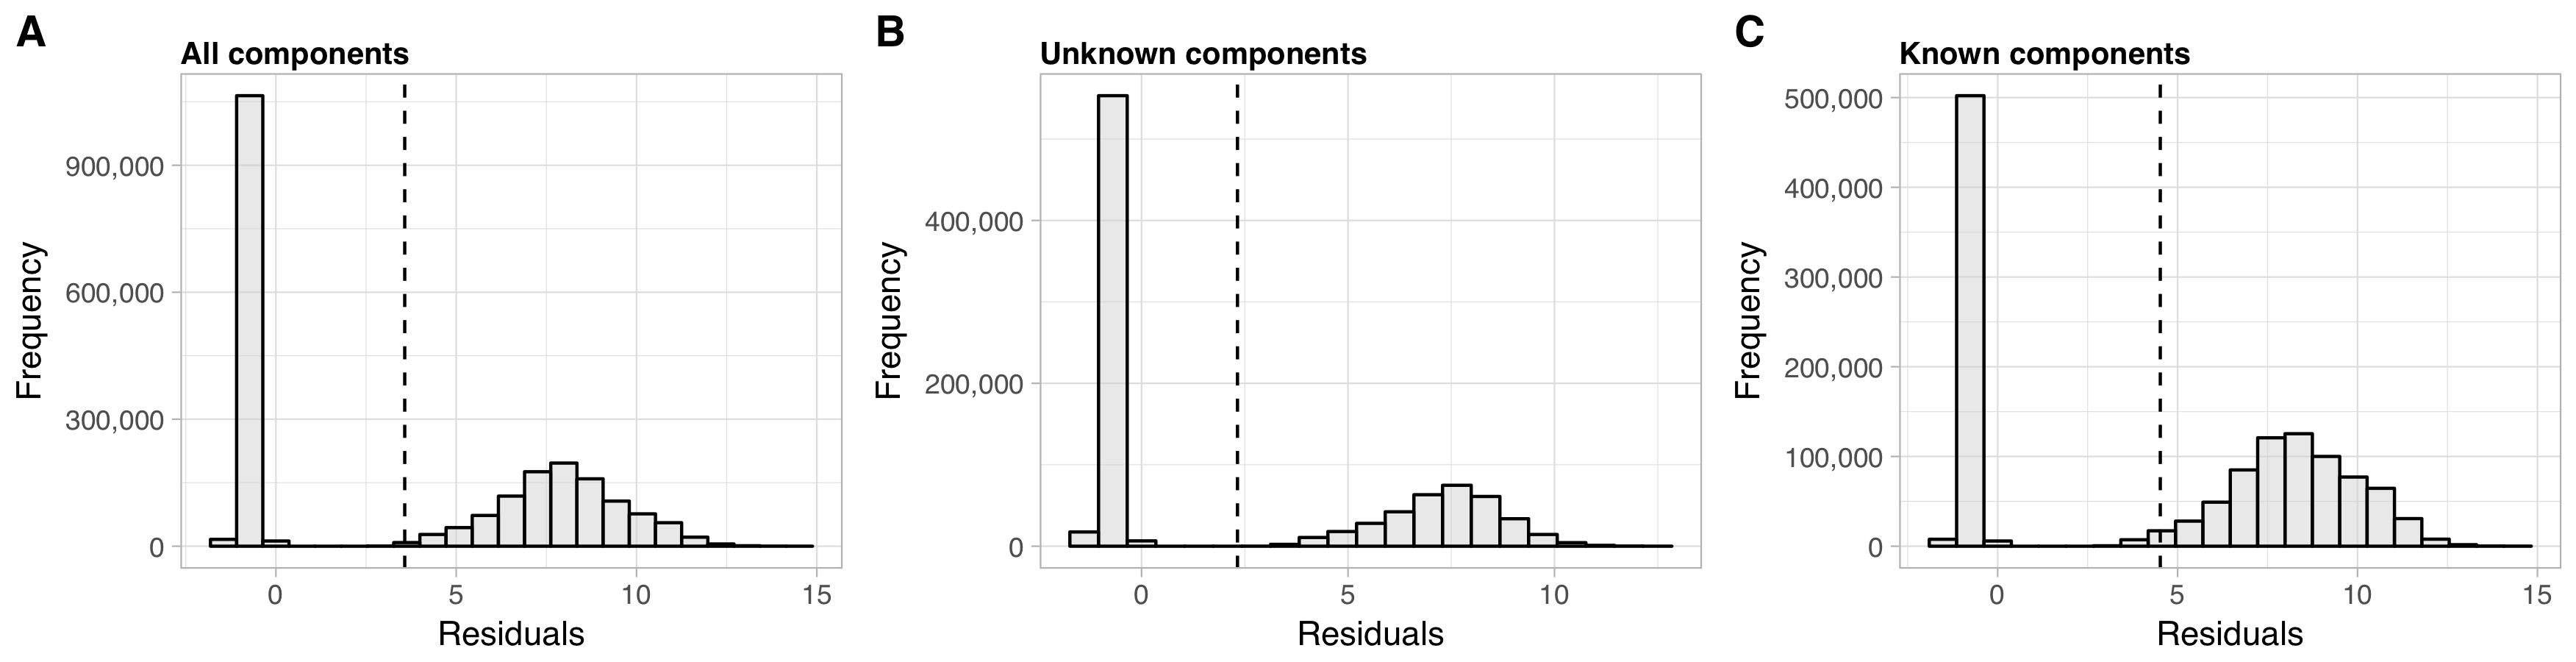
\includegraphics[width=1.0\textwidth] {fig_s1}
	\caption[TARA Oceans PCA residuals histogram]{\textbf{TARA Oceans PCA residuals histogram.} A) Residuals of PCA with sites defined by all components. B) Residuals of PCA with sites defined by at the unknown components (EUs + GUs). C) Residuals of PCA with sites defined by the Known components (K + Kwp).}
	\label{Fig:A1}
\end{figure}

\begin{figure}[h!]
	\centering
	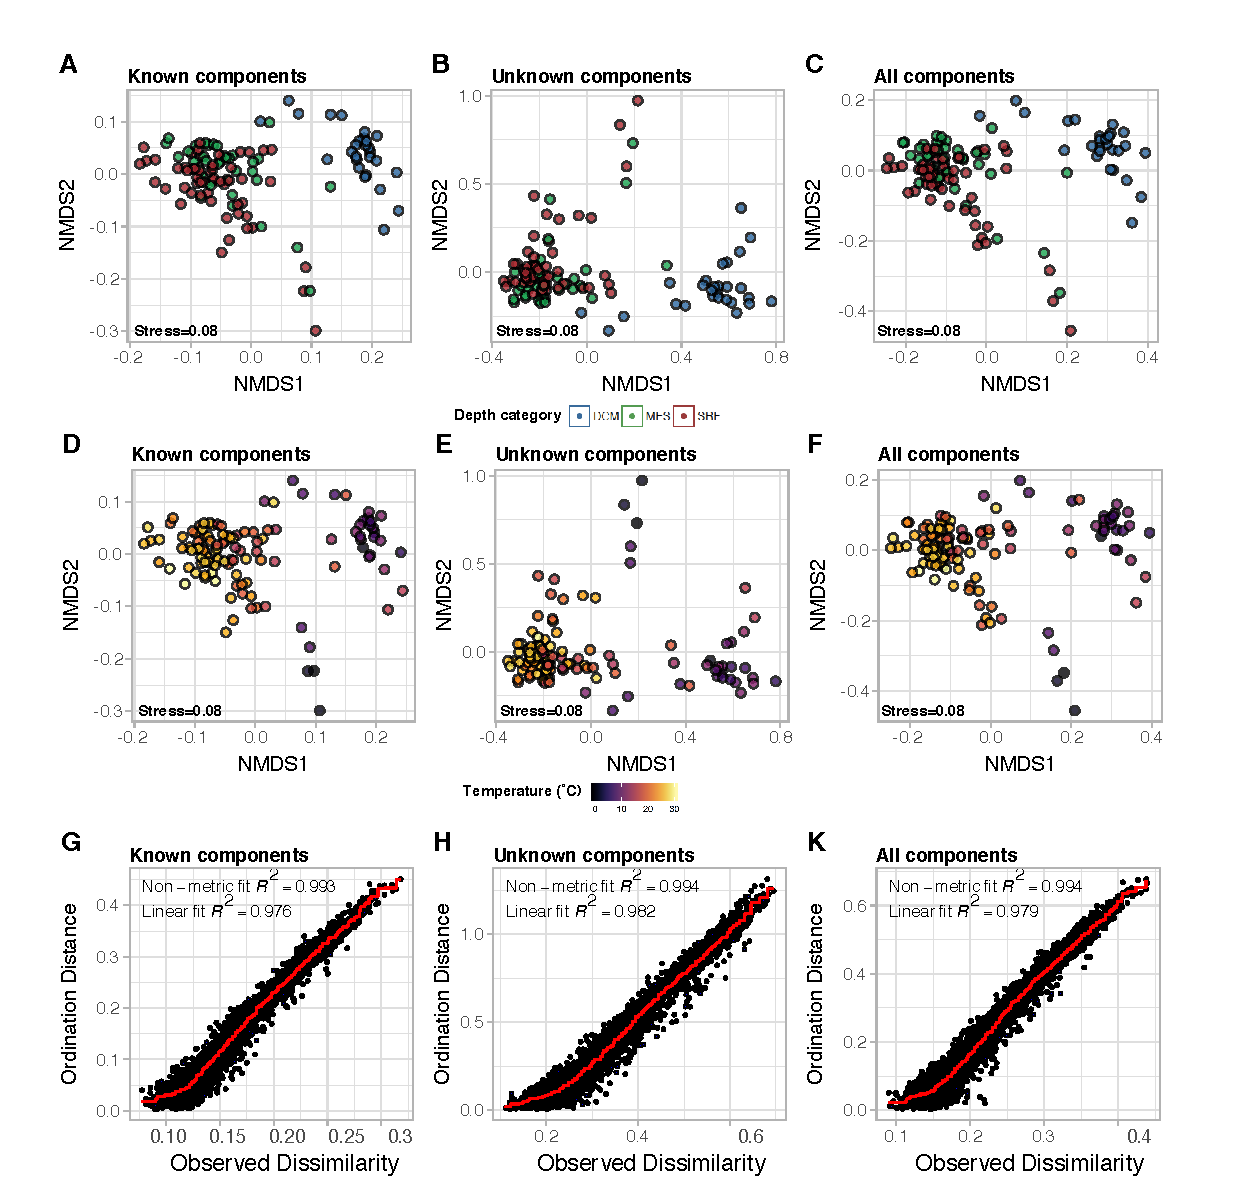
\includegraphics[width=1.0\textwidth] {nmds_panel.pdf}
	\caption[TARA Oceans NMDS and Shepard Plots]{\textbf{TARA Oceans NMDS and Shepard Plots.} A-C) TARA ocean metagenomes defined by (A) Knowns (K + Kwp), (B) Unknowns  (EUs + GUs), and (C) ALL components. Sites are colored by depth of origin (Red = surface, Green = deep chlorophyll maximum, and Blue = mesopelagic. D-E) Same plots as A-C but colored by temperature. The darker the color, the colder the sea water temperature. G-I) Shepard plots for NMDS in A-F }
	\label{Fig:A2}
\end{figure}

\end{appendices}

%\input{Appendices/AppendixB}
%input{Appendices/AppendixC}

%\addtocontents{toc}{\vspace{2em}} % Add a gap in the Contents, for aesthetics

\backmatter{}


%----------------------------------------------------------------------------------------
%	BIBLIOGRAPHY
%----------------------------------------------------------------------------------------
%BIBLIOGRAPHY
%\part{Bibliography}
\addcontentsline{toc}{chapter}{Bibliography}
\bibliographystyle{andreea}
\bibliography{bib.bib}

%% Chapter Template
\cleardoublepage{}
\newpage
\chapter*{Acknowledgements}
\addcontentsline{toc}{chapter}{Acknowledgements}
\label{Acknowledgements}

\pagestyle{empty}
\fancyhead[RE]{}
\fancyhead[LO]{}

To begin, I would like to thank my supervisor Antonio who laid the ground work for me to become a successful PhD student. He has instilled critical thinking and methodical philosophy into my workflow. Where ever I end up I will truly benefit from these last 6 months with him as my supervisor.

A HUGE thanks to Chiara for all the support and not getting tired of me asking questions and barging into her office. 

Next, I would like to thank my two reviewers Frank Oliver and Pier. Thank you for your time and effort for providing me with constructive criticism on this thesis. 

Another thank you to Frank Oliver for allowing me to join the MGG group. I truly enjoyed working with this group and thank you to the whole MGG group for the support!

A separate thank you to Pier who provided with amazing explanations and guidance on my multivariate statistics. 

Thank you Henny for being my MSc partner in crime in MGG.

Thank you to my office mate Marcus Klimmek for all the laughs and drastically improving my German vocabulary in the most important ways.

Thank you to Gerard for working next to me during the beginning. It was fun learning Tidyverse with you!

Thank you MarMic class of 2021 for being an inspirational group of young scientists. I enjoyed learning and growing with you guys and cannot wait see how your careers excel!

Thank you to my coffee amigos Cora, David, and Andrea for all the great conversations and laughs!

Thank you to Christiane and Karl-Heinz for all the MarMic support.

Last but not least, many thanks to my Mother, Father, and Sister who encouraged me all along the way from the other side of the world. 
%\cleardoublepage
\chapter*{Erkl\"arung der selbstst\"andigen Erarbeitung}
\addcontentsline{toc}{chapter}{Erkl\"arung der selbstst\"andigen Erarbeitung}



Hiermit erkl\"{a}re ich, dass ich die Doktorarbeit mit dem Titel:
\textit{My thesis title}

selbstst\"{a}ndig verfasst und geschrieben habe und außer den angegebenen Quellen keine weiteren Hilfsmittel verwendet habe.

Ebenfalls erkl\"{a}re ich hiermit, dass es sich bei den von mir abgegebenen Arbeiten um drei identische Exemplare handelt.

\begin{flushleft}
Bremen, 15 March 2018 \underline{\hspace{6.3cm}}
\hspace*{5cm}(My name)
\end{flushleft}

\begin{flushleft}
\underline{\hspace{6.3cm}} \hspace{2cm} \underline{\hspace{6.3cm}}
\hspace*{3cm}(Date) \hspace{5cm} \hspace*{5cm}(My name)
\end{flushleft}


\end{document}
